%%%%%%%%%%%%%%%%%%%%%%%%%%%%%%%%%%%%%%%%%%%%%%%%%%%
%% LaTeX book template                           %%
%% Author:  Amber Jain (http://amberj.devio.us/) %%
%% License: ISC license                          %%
%%%%%%%%%%%%%%%%%%%%%%%%%%%%%%%%%%%%%%%%%%%%%%%%%%%

\documentclass[a4paper,11pt]{book}
\usepackage[T1]{fontenc}
\usepackage[utf8]{inputenc}
\usepackage{lmodern}
%%%%%%%%%%%%%%%%%%%%%%%%%%%%%%%%%%%%%%%%%%%%%%%%%%%%%%%%%
% Source: http://en.wikibooks.org/wiki/LaTeX/Hyperlinks %
%%%%%%%%%%%%%%%%%%%%%%%%%%%%%%%%%%%%%%%%%%%%%%%%%%%%%%%%%
\usepackage{hyperref}
\usepackage{graphicx}
\usepackage[english]{babel}
\usepackage{amsmath}
\usepackage{amsfonts}
\usepackage{amsthm}
\usepackage{mathtools}
\usepackage{amssymb}
\usepackage{array}
\usepackage{tikz}

%%%%%%%%%%%%%%%%%%%%%%%%%%%%%%%%%%%%%%%%%%%%%%%%
% Chapter quote at the start of chapter        %
% Source: http://tex.stackexchange.com/a/53380 %
%%%%%%%%%%%%%%%%%%%%%%%%%%%%%%%%%%%%%%%%%%%%%%%%
\makeatletter

\renewcommand{\@chapapp}{}% Not necessary...
\newcommand{\Real}{\mathbb{R}}
\newcommand{\Natural}{\mathbb{N}}
\newcommand{\Zahlen}{\mathbb{Z}}
\newcommand{\Quoziente}{\mathbb{Q}}
\newcommand{\newpara}{\\ \newline}
\newcommand{\Complex}{\mathbb{C}}

% inverse hyperbolic functions
\DeclareMathOperator{\sech}{sech}
\DeclareMathOperator{\csch}{csch}
\DeclareMathOperator{\arsec}{arsec}
\DeclareMathOperator{\arcot}{arcot}
\DeclareMathOperator{\arcsc}{arcsc}
\DeclareMathOperator{\arcosh}{arcosh}
\DeclareMathOperator{\arsinh}{arsinh}
\DeclareMathOperator{\artanh}{artanh}
\DeclareMathOperator{\arsech}{arsech}
\DeclareMathOperator{\arcsch}{arcsch}
\DeclareMathOperator{\arcoth}{arcoth} 

\newenvironment{chapquote}[2][2em]
  {\setlength{\@tempdima}{#1}%
   \def\chapquote@author{#2}%
   \parshape 1 \@tempdima \dimexpr\textwidth-2\@tempdima\relax%
   \itshape}
  {\par\normalfont\hfill--\ \chapquote@author\hspace*{\@tempdima}\par\bigskip}
\makeatother

\newtheorem{Theorem}{Theorem}[section]%Theorem
\newtheorem*{Corollary}{Corollary} %Corollary
\newtheorem*{Lemma}{Lemma}%Lemma
\newtheorem{Example}{\textit{Example}}[chapter] % Statement
\theoremstyle{definition}
\newtheorem*{Definition}{Definition} %Definition
\newtheorem*{Proposition}{Proposition}%Proposition

%%%%%%%%%%%%%%%%%%%%%%%%%%%%%%%%%%%%%%%%%%%%%%%%%%%
% First page of book which contains 'stuff' like: %
%  - Book title, subtitle                         %
%  - Book author name                             %
%%%%%%%%%%%%%%%%%%%%%%%%%%%%%%%%%%%%%%%%%%%%%%%%%%%

% Book's title and subtitle
\title{\Huge \textbf{Mathematical Analysis}}
% Author
\author{\textsc{Hechen Hu}}


\begin{document}

\frontmatter
\maketitle
%%%%%%%%%%%%%%%%%%%%%%%%%%%%%%%%%%%%%%%%%%%%%%%%%%%%%%%%%%%%%%%%%%%%%%%%
% Auto-generated table of contents, list of figures and list of tables %
%%%%%%%%%%%%%%%%%%%%%%%%%%%%%%%%%%%%%%%%%%%%%%%%%%%%%%%%%%%%%%%%%%%%%%%%
\tableofcontents

\mainmatter

%%%%%%%%%%%%%%%%
% NEW CHAPTER! %
%%%%%%%%%%%%%%%%
\chapter{General Mathematical Concepts and Notation}

\section{Mathematical Symbols and their meanings}
\begin{tabular}{| l | l |}
	\hline
	Notation &Meaning\\ \hline
	$L\Rightarrow P$ &L implies P \\ \hline
	$L\Leftrightarrow P$ &L is equivalent to P \\ \hline
	$((L\Rightarrow P)\land(\lnot P))\Rightarrow(\lnot L)$ &If P follows from L and P is false, then L is false \\ \hline
	$\lnot((L\Leftrightarrow G)\lor(P\Leftrightarrow G)$ &G is not equivalent either to L or to P \\ \hline
	$A \coloneqq B$ &The Definition of A is B (equality by definition)\\ \hline
	$\square$ &End of proof \\
	\hline
\end{tabular}

\section{Sets and Operations on Them}

\subsection{Naive Set Theory}
1$^0$.\quad A set may consist of any distinguishable objects($x\in A\Rightarrow\exists!x\in A$) \\
2$^0$.\quad A set is unambiguously determined by the collection of objects that comprise it. \\
3$^0$.\quad Any property defines the set of objects having that property($A = \{x|P(x)\}\Rightarrow P(A)$). \\ \\
However, this will lead to Russell's Paradox: \\
Let's have$P(M) \coloneqq M\notin M$ \\
Consider the class $K = \{M|P(M)\}$. If so $K$ is not a set, since whether $P(K)$ is true or false, contradiction arises.\\

\subsection{ZFC: Zermelo-Fraenkel Axioms and Axiom of Choice}
1$^0$.\quad \textbf{(Axiom of Extensionality)} Sets $ A $ and $B$ are equal iff they have the same elements. $ (A=B)\Leftrightarrow(\forall x((x\in A)\Leftrightarrow(x \in B))) $\\
2$^0$. \quad \textbf{(Axiom of Seperation)} To any set $A$ and any property P there corresponds a set $B$ whose elements are those elements of $A$, and only those, having property P(if $A$ is a set, then $B=\{x\in A|P(x)\}$ is also a set). \\
3$^0$. \quad \textbf{(Union Axiom)} For any set $ M $ whose elements are sets there exists a set $\bigcup M$, called the union of $ M $ and consisting of those elements and only those that belong to some element of $ M $ $ (x\in \bigcup M \Leftrightarrow \exists X((X\in M)\land (x\in X))) $ \\
Similarly, the intersection of the set $ M $ is defined as:
\begin{equation}
	\bigcap M  \coloneqq \{x\in \bigcup M | \forall X((X\in M)\Rightarrow (x\in X))\} \nonumber
\end{equation}
4$^0$ \quad \textbf{(Pairing Axiom)} For any sets $ X $ and $ Y $ there exists a set $ Z $ such that $ X $ and $ Y $ are its only elements. \\
5$^0$ \quad \textbf{(Power Set Axiom)} For any set $ X $ there exists a set $ P(X)$ having each subset of $ X $ as an element, and having no other elements. \\
\newline
\begin{Definition}
The \textit{successor} $X^+$ of the set $ X $ is $X^+ = X\cup \{X\}$.\\
\end{Definition} 
\begin{Definition}
An \textit{inductive} set is a set that $\varnothing$ is one of its elements and the successor of each of its elements aso belongs to it.
\end{Definition}
6$^0$ \quad \textbf{(Axiom of Infinity)} There exist inductive sets (Example: $\mathbb{N}_0$).\\ 
7$^0$ \quad \textbf{(Axiom of Replacement)} Let $ F(x,y) $ be a statement(a formula) such that for every $ x_0 \in X$ there exists a unique object $ y_0 $ such that $ F(x_0,y_0) $ is true. Then the objects $ y $ for which there exists an element $ x\in X $ such that $ F(x,y) $ is true form a set.\\
And finally, an axiom that is independent of ZF. \\
\newline
\begin{Definition}
A choice function is a function $ f $, defined on a collection $ X $ of nonempty sets, such that for every set $ A $ in $ X $, $ f(A) $ is an element of $ A $.
\end{Definition}
8$^0$ \quad \textbf{(Axiom of Choice/Zermelo's Axiom)}  For any set $ X$ of nonempty sets, there exists a choice function $ f $ defined on $ X $.$(\forall X[\varnothing \notin X \Rightarrow \exists f: X\mapsto \bigcup X \quad \forall A\in X(f(A)\in A)])$

\subsection{The \textit{Cardinality} of a Set(\textit{Cardinal Numbers})}
\begin{Definition}
The set $ X $ is said to be \textit{equipollent} to the set $ Y $ if there exists a bijective mapping of $ X $ onto $ Y $(then $ X\sim Y $).
\end{Definition}
\begin{Definition}
\textit{Cardinality} is a measure of the number of elements of the set. If $ X \sim Y $, we write $ card X = card Y $.
\end{Definition}
If $ X $ is equipollent to some subset of $ Y $, we say $ card X\leqslant card Y $, thus
\begin{equation}
	(card X \leqslant card Y)\coloneqq \exists Z\subset Y (card X = card Z) \nonumber
\end{equation}
A set is called \textit{finite} if it is not equipollent to any proper subset of itself; otherwise it is called \textit{infinite}. \\
It has the  properties below:\\
\newline
1$^0  \quad (cardX\leqslant card Y)\land(card Y \leqslant card Z)\Rightarrow(card X \leqslant card Z)$.\\
2$^0 \quad (card X \leqslant card Y)\land(card Y \leqslant card X)\Rightarrow(card X = card Y)$(The Schröder–Bernstein theorem).\\
3$^0 \quad \forall X\forall Y(card X \leqslant card Y)\lor(card Y \leqslant card X)$(Cantor's theorem).\\
\newline
We say $ card X < card Y $ if $ (card X \leqslant card Y) \land (card X \neq card Y)$.\\
let $ \varnothing $ be the empty set and $ P(X) $ the set of all subsets(thus, the power set) of the set $ X $. Then:
\begin{Theorem}
	$ card X < card P(X) $
\end{Theorem}
\begin{proof}
The assertion is obvious for the empty set, and we shall assume that $ X\neq \varnothing $.\\
Since $ P(X) $ contains all the one-element subsets of $ X $, $ cardX \leqslant cardP(X)$.\\
Suppose, contrary to the assertion, that there exists a bijective mapping $ f : X \to P(X) $. Let set $ A = \{x\in X:x\notin f(x)\}$ consisting of the elements $ x \in X $ that do not belong to the set $ f(x)\in P(X) $ assigned to them by the bijection. Because $ A \in P(X) $, there exists $ a\in X $ such that $ f(a) = A $. For the element $ a $ the relation $ a \in A $ or $ a \notin A $ is impossible by the definition of $ A $(Similar to Russell's Paradox).
\end{proof}



\subsection{Operations on Sets}
\begin{tabular}{| l | l | l |}
	\hline
	Notation &Meaning &Definition \\ \hline
	$A\subset B$ &$A$ is a subset of $B$ &$\forall x ((x\in A) \Rightarrow(x\in B))$ \\ \hline
	$A = B$ &$A$ equals to $B$ &$(A \subset B)\land(B \subset A)$ \\ \hline
	$\varnothing$ &Empty Set & $\{x|x\neq x\}$ \\ \hline
	$A \cup B$ &The union of $ A $ and $ B $ &$ \{x|x\in A \lor x\in B\} $ \\
	$ A \cap B $ &The intersection of $ A $ and $ B $ &$ \{x|x\in A \land x\in B\} $ \\ \hline
	$ A\setminus B $ &The difference between $ A $ and $ B $ &$ \{x|x\in A \land x\notin B\} $ \\ \hline
	$ C_M A $ &The complement of $A$ in M &$ \{x|x\in M \land x\notin A\} where A\subset M $ \\ \hline
	$ A \times B $ &The Cartesian Product of $ A $ and $ B $ &$ \{(x,y)|x\in A \land y\in B\} $ \\ \hline
	$ A^2 $ &$ A \times A $ & \\
		\hline
\end{tabular}
 \newline \\
In the ordered pair$ z = (x_1,x_2) $ where$ Z = X_1 \times X_2 ,z\in Z,x_1 \in X_1, x_2 \in X_2$, $ x_1 $ is called the \textit{first projection} of the pair $ z $ and denoted  pr$_1 z $ while $ x_2 $ is called the \textit{second projection} of the pair $ z $ and denoted  pr$_2 z $.






\section{Relations and Functions}
\subsection{Definitions of Functions}
\begin{Definition} 
We say that there is a \textit{function} defined on $ X $ with values in $ Y $ if, by virtue of some fule $ f $, to each element $ x\in X $ there corresponds an element $ y \in Y $.
\begin{equation}
f(X) \coloneqq \{y \in Y | \exists x((x\in X)\land(y = f(x)))\} \nonumber
\end{equation}
X is called the \textit{domain of definition} and Y is called \textit{set of values} or \textit{range} of the function.
\end{Definition}
\begin{Definition}
If $ A \subset X$ and $ f:X \to Y $ is a function. We denote by $ f|_A $ the function $ \varphi:A \to Y $ that agrees with $ f $ on $ A $. More precisely, $ f|_A(x) \coloneqq \varphi(x)$ if $ x\in A  $. The function $ f|_A $ is called the restriction of $ f $ to $ A $, and the function $ f:X \to Y $ is called an extension or a continuation of $ \varphi $ to $ X $.
\end{Definition}

We use the term \textit{domain of departure} of the function to denote any set $ X $ containing the domain of a function, and \textit{domain of arrival} to denote any subset of $ Y $ containing its range.

\subsection{Elementry Classification of Mappings}
\begin{Definition}
When a function $ f: X\to Y $ is called a mapping, the value $ f(x) \in Y $ that it assumes at the element $ x \in X$ is usually called the \textit{image} of $ x $. \\
The \textit{image} of a set $ A \subset X $ under the mapping $  f: X\to Y $ is defined as the set
\begin{equation}
f(A) \coloneqq \{y\in Y | \exists x((x\in A)\land(y = f(x))\} \nonumber
\end{equation}
consisting of the elements of $ Y $ that are images of elements of $ A $.
\end{Definition} 

The set
\begin{equation}
	f^{-1}(B)\coloneqq \{x\in X | f(x)\in B\} \nonumber
\end{equation}
consisting of the elements of $ X $ whose images belong to $ B $ is called the \textit{pre-image} (or \textit{complete pre-image}) of the set $ B \subset Y $. \\
\newline
\begin{Definition}
A mapping $  f: X\to Y  $ is said to be \\
\textit{surjective} if $ f(X) = Y $\\
\textit{injective} if $ \forall x_1,x_2 \in X $, $(f(x_1)=f(x_2))\Rightarrow(x_1=x_2)$ holds.\\
\textit{bijective} if it's both surjective and injective.	
\end{Definition}

\begin{Definition}
The inverse mapping of a bijective $ f $ is denoted as
\begin{equation}
f^{-1}:Y\to X \nonumber
\end{equation}
and defined as follows: if $ f(x) = y $, then $ f^{-1}(y) = x $. 
\end{Definition}
Note that the pre-image of a set is defined for any mapping $ f:X\to Y $, even if it is not bijective and hence has no inverse.

\subsection{Composition of Functions and Mutually Inverse Mappings}
\begin{Definition}
For two mappings $ f:X\to Y $ and $ g:Y \to Z $,
\begin{equation}
g \circ f:X \to Z,\quad (g \circ f)(x)\coloneqq g(f(x)) \nonumber
\end{equation}
is called the \textit{composition} of the mapping $ f $ and the mapping $ g $.	
\end{Definition}

If all the terms of a composition $ f_n \circ ... \circ f_1 $ are equal to the same function $ f $, we abbreviate it to $ f^n $.\\
\newline
Function composition is associative, that is,
\begin{equation}
	h \circ (g\circ f) = (h \circ g)\circ f \nonumber
\end{equation}
But in general, $ g\circ f \neq f \circ g $. \\
\newline
\begin{Definition}
The mapping $ f:X \to X $ that assigns each element in $ X $ to itself is called the \textit{identity mapping} on $ X $ and denoted $ e_X $.
\end{Definition} 
\begin{Lemma}
	$	(g\circ f = e_X) \Rightarrow$($g$ is surjective) $\land$ ($f$ is injective).
\end{Lemma}

\begin{proof}
	If $ f:X\to Y$,$ g:Y\to X $, and $ g \circ f = e_X:X\to X $, then
	\begin{equation}
		X = e_X(X) = (g\circ f)(X) = g(f(X))\subset g(Y) \nonumber
	\end{equation}
	and hence $ g $ is surjective. \\
	Further, if$ x_1\in X $ and $ x_2 \in X $, then
	\begin{align}
		(x_1\neq x_2) &\Rightarrow (e_X(x_1)\neq e_X(x_2))\Rightarrow((g\circ f)(x-1)\neq (g\circ f)(x_2))\Rightarrow \nonumber \\
							 &\Rightarrow (g(f(x_1))\neq g(f(x_2))) \Rightarrow(f(x_1)\neq f(x_2)) \nonumber
	\end{align}
	and therefore $ f $ is injective.
\end{proof}

\begin{Proposition}
The mappings $ f :X\to Y $ and $ g:Y\to X $ are bijective and mutually inverse to each other if and only if $ g \circ f = e_X $ and $ f \circ g = e_Y $.
\end{Proposition}


\subsection{Functions as Relations. The Graph of a Function}
\subsubsection{Relations}
\begin{Definition}
A Relation $ R $ is any set of ordered pairs $ (x,y) $. \\
The set $ X $ is called the \textit{domain of definition} of $ R $, and the set $ Y $ is the \textit{range of values}. 
\end{Definition}
Any set containing the domain of definition of a relation is called a \textit{domain of departure} for that relation, and \textit{domain of arrival} is a set that contains the range of values of the relation. \\
\newline
Instead writing $ (x,y)\in R $, we write $ xRy $ and say that $ x $ is \textit{connected with} $ y $ \textit{by the relation $ R $}.\\
If $ R \subset X^2 $, then we say that the relation $ R $ is defined on $ X $.

\subsubsection{Classification of Relations}
\begin{Definition}
An \textit{equivalence relation} is a relation that satisfy the following properties: \\
\newline
$ aRa $ (Reflexivity);\\
$ aRb \Rightarrow bRa $ (Symmetry); \\
$ (aRb)\land (bRc) \Rightarrow aRc $ (Transitivity).\\
\newline
An equivalence relation is denoted by the special symbol $ \sim $. $ a\sim b $ means $ a $ is \textit{equivalent} to $ b $.	
\end{Definition}

\begin{Definition}
A \textit{partial ordering} on a set $ X^2 $ is a relation $ R $ that have the following properties: \\
\newline
$ aRa $ (Reflexivity);\\
$ (aRb)\land (bRc) \Rightarrow aRc $ (Transitivity).\\
$ (aRb) \land (bRa )\Rightarrow (a=b) $ (Anti-symmetry);	
\end{Definition}

We often write $ a\preceq b $ and say that $ b $ \textit{follows} $ a $.
If the condition
\begin{equation}
	\forall a \forall b((aRb)\lor(bRa) \nonumber
\end{equation}
holds in addition to transitivity and anti-symmetry defining a partial ordering relation(this means any two elements of $ X $ is comparable), the relation $ R $ is called an \textit{ordering}, and the set $ X $ is said to be \textit{linearly ordered}.

\subsubsection{Functions and Their Graphs}
\begin{Definition}
	A relation $ R $ is said to be functional if
	\begin{equation}
	(xRy_1)\land(xRy_2)\Rightarrow (y_1=y_2) \nonumber
	\end{equation}
	and it is called a \textit{function}.\\
	$ R\subset X \times Y $ is a \textit{mapping from $ X $ into $ Y $}, or a \textit{function from $ X $ into $ Y $}.\\
\end{Definition}

\begin{Definition}
The \textit{graph} of a function $ f:X \to Y $, is the subset $ \Gamma $ of $ X \times Y $.
\begin{equation}
\Gamma \coloneqq \{(x,y)\in X \times Y | y = f(x)\} \nonumber
\end{equation}
\end{Definition} 


\chapter{The Real Numbers}
\section{The Axiom System and Some General Properties of the Set of Real Numbers}
\subsection{The Axiom System of the Real Numbers}
\subsubsection{Axioms for Addition:} An operation 
\begin{equation}
	+:\Real \times \Real \to \Real \nonumber
\end{equation}
is defined, assgining to each ordered pair $ (x,y) $ of elements $ x,y $ of $ \Real $ a certain element $ x+y \in \Real $. \\
1$_+ $\quad There exists a neutral, or identity element $ 0 $ (called zero) such that 
\begin{equation}
	x+0 = 0+x = x \nonumber
\end{equation} for every $ x \in \Real $. \\
2$ _+ $\quad For every element $ x\in \Real $ there exists an element $ -x\in \Real $ called the \textit{negative of $ x $}.
\begin{equation}
	\forall x \in \Real \Rightarrow (\exists! (-x)\in \Real)\land (x +(-x) = (-x)+x=0) \nonumber
\end{equation}
3$ _+ $\quad The operation $ + $ is associative.
\begin{equation}
	\forall x \forall y \forall z \in \Real \Rightarrow x+(y+z) = (x+y)+z \nonumber
\end{equation}
4$ _+ $\quad The operation $ + $ is commutative.
\begin{equation}
	\forall x \forall y \in \Real \Rightarrow(x+y = y+x) \nonumber
\end{equation}
\newline
\begin{Definition}
A group structure is defined on the set $ G $ -- or $ G $ is a group -- if Axioms 1$_+ $, 2$ _+ $, and 3$ _+ $ holds for an operation defined on this set. The group is called \textit{additive} group if the operation is called addition. When the operation is also commutative, that is, Axiom 4$ _+ $ holds, the group is also called a \textit{commutative group} or an \textit{Abelian group}. 
\end{Definition}
According to Axioms 1$ _+ $ -- 4$ _+ $, $ \Real $ is an additive Abelian group.\\
\subsubsection{Axioms for Multiplication:} An operation 
\begin{equation}
	\bullet:\Real \times \Real \to \Real \nonumber
\end{equation}
is defined, assigning to each ordered pair $ (x,y) $ of elements $ x,y\in \Real $ a certain element $ x \cdot y \in \Real $, called the product of $ x $ and $ y $. \\
1$ _\bullet $\quad There exists a neutral, or identity element $ 1 \in \Real\setminus 0 $ such that
\begin{equation}
	\forall x \in \Real \Rightarrow (x \cdot 1 = 1 \cdot x = x) \nonumber
\end{equation}
2$ _\bullet $\quad  For every element $ x \in \Real\setminus 0 $ there exists an element $ x^{-1}\in \Real $, called the \textit{inverse} or \textit{reciprocal} of $ x $.
\begin{equation}
	\forall x \in \Real \Rightarrow (x\cdot x^{-1} = x^{-1} \cdot x = 1) \nonumber
\end{equation}
3$ _\bullet $\quad The operation $ \bullet $ is associative.
\begin{equation}
	\forall x \forall y \forall z \in \Real \Rightarrow x\cdot(y\cdot z) = (x\cdot y)\cdot z \nonumber
\end{equation}
4$ _\bullet $\quad The operation $ \bullet $ is commutative.
\begin{equation}
	\forall x \forall y \in \Real \Rightarrow x\cdot y = y \cdot x \nonumber
\end{equation}
The set $ \Real \setminus 0 $ is a \textit{multiplicative} group. \\
\newline
Multiplication is distributive with respect to addition.
\begin{equation}
		\forall x \forall y \forall z \in \Real \Rightarrow (x+y)z = xz+yz \nonumber
\end{equation}
\begin{Definition}
If two operations satisfying the Axioms of Addition and Multiplication are defined on a set $ G $, then $ G $ is called a \textit{field}.
\end{Definition}
\subsubsection{Order Axioms}
Between elements of $ \Real $ there is a relation $ \leqslant $ defined, and :\\
0$ _{\leqslant} $\quad $ \forall x \in\Real(x\leqslant x) $ (Reflexivity) \nonumber \\
1$ _{\leqslant} $\quad $ (x \leqslant y)\land (y \leqslant x) \Rightarrow (x=y) $(Anti-Symmetry)\nonumber \\
2$ _{\leqslant} $\quad $ (x \leqslant y) \land (y \leqslant z) \Rightarrow (x \leqslant z) $ (Transitivity)\nonumber \\
3$ _{\leqslant} $\quad $ \forall x \in \Real \forall y \in \Real(x\leqslant y)\lor(y\leqslant x) $\nonumber \\
Thus, the relation $ \leqslant $ is an ordering, and $ \Real $ is linearly ordered.
\subsubsection{The Connection between Addition and Order on $ \Real $}
\begin{equation}
	\forall x \forall y \forall z \in \Real \Rightarrow ((x\leqslant y)\Rightarrow (x +z \leqslant y + z) \nonumber
\end{equation}
\subsubsection{The Connection between Multiplication and Order on $ \Real $}
\begin{equation}
\forall x \forall y \in \Real \Rightarrow ((0\leqslant x)\land (0 \leqslant y)\Rightarrow(0 \leqslant x \cdot y)) \nonumber
\end{equation}
\subsubsection{The Axiom of Completeness(Continuity)}
If $ X $ and $ Y $ are nonempty subsets of $ \Real $ having the property that $ x \leqslant y $ for every $ x \in X $ and every $ y \in Y $, then there exists $ c\in \Real $ such that $ x\leqslant c \leqslant y $ for all $ x \in X $ and $ y \in Y $.
\begin{equation}
	(\forall X \forall Y\subset \Real)\land(X,Y \neq \varnothing)\land(\forall x\in X \forall y \in Y \Rightarrow x \leqslant y)\Rightarrow (\exists c\in \Real \forall x\in X \forall y \in Y (x \leqslant c \leqslant y)) \nonumber
\end{equation}
\newline
\textbf{Any set on which these axioms hold can be considered a \textit{model} of the real numbers.} \\
\newline
\begin{Definition}
An axiom system is said to be \textit{categorical} if it determines an unique mathematical object.
\end{Definition}

\begin{Definition}
If there are two models of independent number systems $ \Real_A $ and $ \Real _B $ that satisfying all the axioms, then a bijective correspondence can be established between these two systems, say $ f:\Real_A \to \Real_B $, preserving the arithmetic operations and the order, that is, 
\begin{align}
f(x+y) &= f(x) + f(y)\nonumber \\
f(x\cdot y) &= f(x) \cdot f(y) \nonumber \\
x\leqslant y &\Leftrightarrow f(x) \leqslant f(y) \nonumber 
\end{align}
and we can say that $ \Real_A $ and $ \Real _B $ are \textit{isomorphic} and the mapping $ f $ is called an \textit{isomorphism}.
\end{Definition} 

\begin{Theorem}
	The Axiom System of The Real Numbers is categorical.
\end{Theorem}

\subsection{Some General Algebraic Properties of Real Numbers}
\subsubsection{Consequences of the Addition Axioms}
1$ ^0 $\quad There is only one zero in the set of real numbers.\\
2$ ^0 $\quad Each element of the set of real numbers has a unique negative.\\
3$ ^0 $\quad In $ \Real $ the equation
\begin{equation}
	a + x = b \nonumber
\end{equation}
has the unique solution 
\begin{equation}
	x = b+(-a) \nonumber
\end{equation}

\subsubsection{Consequences of the Multiplication Axioms}
1$ ^0 $\quad There is only one multiplicative unit in the real numbers.\\
2$ ^0 $\quad For each $ x \neq 0 $ there is only one reciprocal $ x^{-1} $.\\
3$ ^0 $\quad For $ a\in \Real\setminus 0 $, the equation $ a\cdot x = b $ has the unique solution $ x = b\cdot a^{-1} $.

\subsubsection{Consequences of the Axiom Connecting Addition and Multiplication}
1$ ^0 $\quad For any $ x\in \Real $ 
\begin{equation}
	x\cdot 0 = 0 \cdot x = 0 \nonumber
\end{equation}
2$ ^0 $\quad $ (x\cdot y = 0)\Rightarrow(x=0)\lor(y=0) $. \\
3$ ^0 $\quad For any $x \in \Real  $
\begin{equation}
	-x = (-1)\cdot x \nonumber
\end{equation}
4$ ^0 $\quad For any $ x\in\Real $
\begin{equation}
	(-1)\cdot(-x)=x \nonumber
\end{equation}
5$ ^0 $\quad For any $ x\in \Real $
\begin{equation}
	(-x)\cdot(-x) = x\cdot x \nonumber
\end{equation}

\subsubsection{Consequences of the Order Axioms}
1$ ^0 $\quad For any $ x $ and $ y $ in $ \Real $ precisely one of the following relations holds:
\begin{equation}
	x < y, \quad x = y,\quad x>y \nonumber
\end{equation}
2$ ^0 $\quad For any $ x,y,z\in\Real $
\begin{align}
	(x<y)\land(y\leqslant z) &\Rightarrow (x<z) \nonumber \\	
	(x\leqslant y)\land(y< z) &\Rightarrow (x<z) \nonumber
\end{align}

\subsubsection{Consequences of the Axiom Connecting Order with Addition and Multiplication}
1$ ^0 $\quad For any $ x,y,z,w\in \Real $
\begin{align}
	(x<y)&\Rightarrow(x+z)<(y+z)\nonumber \\
	(0<x)&\Rightarrow(-x<0) \nonumber\\
	(x\leqslant y)\land(z\leqslant w)&\Rightarrow (x+z)\leqslant(y+w)\nonumber \\
	(x< y)\land(z<w)&\Rightarrow (x+z)<(y+w)\nonumber \\
\end{align}
2$ ^0 $\quad If $ x,y,z \in \Real $,then
\begin{align}
	(0<x)\land(0<y)&\Rightarrow(0<xy) \nonumber \\
	(x<0)\land(y<0)&\Rightarrow(0<xy) \nonumber \\
	(x<0)\land(0<y)&\Rightarrow(xy<0) \nonumber \\
	(x<y)\land(0<z)&\Rightarrow(xz<yz)\nonumber \\
	(x<y)\land(z<0)&\Rightarrow(yz<xz)\nonumber
\end{align}
3$ ^0 $\quad $0<1$. \\
4$ ^0 $\quad $ (0<x)\Rightarrow(0<x^{-1}) $ and $ (0<x)\land(x<y)\Rightarrow(0<y^{-1})\land(y^{-1}<x^{-1}) $.

\subsection{The Completeness Axiom and the Existence of a Least Upper(or Greatest Lower) Bound of a Set of Numbers}
\begin{Definition}
	A set $ X\subset \Real $ is said to be \textit{bounded above} (resp. \textit{bounded below}) if there exists a number $ c\in\Real $ such that $ x\leqslant c $(resp.$ c\leqslant x $) for all $ x\in X $.
\end{Definition}
\begin{Definition}[Maximal and Minimal Elements]
	\begin{align}
	(a= maxX)&\coloneqq(a\in X\land \forall x\in X(x\leqslant a))\nonumber \\
	(a= minX)&\coloneqq(a\in X\land \forall x\in X(a\leqslant x))\nonumber \\
	\end{align}
	It follows from the order Axiom 1$ _\leqslant $ that if there is a maximal (resp. minimal ) element in a set of numbers, it is the only one. \\
	However, not every set, not even every bounded set, has a maximal or minimal element(e.g. $ X = \{x\in R|0\leqslant x<1\} $).
\end{Definition}
\begin{Definition}
	The smallest number that bounds a set $ X\subset \Real $ from above is called the \textit{least upper bound}(or the \textit{eact upper bound}) of $ X $ and denoted $ \sup X $("the supremum of $ X $").
	\begin{equation}
	(s=\sup X)\coloneqq \forall x\in X((x\leqslant s)\land(\forall s^\prime<s\exists x^\prime \in X (s^\prime < x^\prime)))\nonumber
	\end{equation}
	Similarly, the greatest lower bound of $ X $, $ \inf X $("the infimum of $ X $) can be defined as:
	\begin{equation}
	(i=\inf X)\coloneqq \forall x\in X((i\leqslant x)\land(\forall i^\prime>i\exists x^\prime \in X (x^\prime < i^\prime)))\nonumber
	\end{equation}
\end{Definition}\textbf{}
\begin{Lemma}
	(The least upper bound principle) Every nonempty set of real numbers that is bounded from above has a unique least upper bound.
\end{Lemma}
\begin{proof}
	Since we already know that the minimal element of a set of numbers is unique(the relation $ \leqslant $ is Anti-Symmetric), we need only verify that the least upper bound exists.\\
	Let $ X\subset \Real $ be a given set and $ Y = \{y\in \Real|\forall x\in X (x \leqslant y)\} $. We know that $ X \neq \varnothing $ and $ Y \neq \varnothing $. Then, by the completeness axiom there exists $ c \in R $ such that $ \forall x \in X \forall y \in Y (x\leqslant c \leqslant y) $. Because $ c $ is  greater than all the elements in $ X $ and smaller than all the elements in $ Y $, we can see that $ c \in Y$ and $ c = min Y $. $ \forall c^\prime < c $ we have $ c^\prime \in X $, and according to the completeness axiom of real numbers, there exists some $ x^\prime \in X$ such that $ c^\prime \leqslant x^\prime \leqslant c $. Thus $ c $ is $ \sup X $.
\end{proof}
The existence of greatest lower bound is analogous with the existence of least upper bound, so
\begin{Lemma}
	($ X $ is nonempty and bounded below)$ \Rightarrow(\exists! \inf X) $.
\end{Lemma}









\section{The Most Important Classes of Real Numbers and Computational Aspects of Operations with Real Numbers}
\subsection{The Natural Numbers and the Principle of Mathematical Induction}
\subsubsection{Definition of the Set of Natural Numbers}
\begin{Definition}
	A set $ X\subset \Real $ is \textit{inductive} if for each number $ x\in X $, it also contains $ x+1 $.
\end{Definition}

\begin{Definition}
	The set of \textit{natural numbers} is the smallest inductive set(has the cardinality of $ \aleph_0 $) containing $ 1 $, that is, the intersection of all inductive sets that contain $ 1 $.
\end{Definition}

\subsubsection{The Principle of Mathematical Induction}
\begin{Definition}
	If a subset $ E $ of the set of natural numbers $ \Natural $ is such that $ 1 \in E $ and together with each number $ x\in E $, the number $ x+1 $ also belongs to $ E $, then $ E=\Natural $.
	\begin{equation}
		(E\subset \Natural)\land(1\in E)\land(x\in E \Rightarrow (x+1)\in E)\Rightarrow E = \Natural \nonumber
	\end{equation}
\end{Definition}
Some properties of the natural numbers:\\
1$ ^0 $\quad The sum and product of natural numbers are natural numbers.\\
2$ ^0 $\quad $ (n\in \Natural)\land(n\neq 1)\Rightarrow ((n-1)\in \Natural) $. \\
3$ ^0 $\quad For any $ n\in \Natural $ the set $ \{x\in \Natural | n <x\} $ contains a minimal element, namely
\begin{equation}
	min\{x\in \Natural | n <x\} = n+1 \nonumber
\end{equation}
4$ ^0 $\quad $ (n\in\Natural)\land(m \in \Natural)\land(n<m)\Rightarrow(n+1\leqslant m) $.\\
5$ ^0 $\quad The number $ (n+1)\in\Natural $ is the immediate successor of the number $ n\in \Natural $; that is, if $ n\in \Natural $, there are no natural numbers $ x $ satisfying $ n-1<x<n $. \\
6$ ^0 $\quad If $ n\in \Natural $ and $ n\neq 1 $, then $ (n-1)\in \Natural $ and $ (n-1) $ is the immediate predecessor of $ n\in \Natural $; that is , if $ n\in \Natural $, there are no natural numbers $ x $ satisfying $ n-1<x<n $.\\ 
7$ ^0 $\quad In any nonempty subset of $ \Natural $ there is a minimal element.\\
\begin{proof}
	Let $ M \subset \Natural $. \\
	Case 1: For $ 1\in M $, We'll have $ minM $ = 1, since $ \forall n \in \Natural (1\leqslant n)$. \\
	Case 2: For $ 1 \notin M $, we find a set $ E $ such that $ 1 \in E = \Natural \setminus M $. If $ n $ is $ max E $, then $ \forall e \in E \Rightarrow e \leqslant n $. However, $ (n+1) \notin E $ because $ \forall n \in \Natural\Rightarrow(n+1)>n $, and thus $ (n+1)\in M $ (If such $ n $ do not exist, then $ E $  which contains $ 1 $ is not bounded from above, and we can see that $ (n\in E) \Rightarrow ((n+1)\in E) $. By the principle of induction, $ E = \Natural $. But this is impossible, since $ \Natural \setminus E = M \neq \varnothing $). \\
	Therefore, $ (\forall x\in M)\Rightarrow (n\nleqslant x\nleqslant (n+1) ) \Rightarrow  (min M = (n+1)) $ .
\end{proof}

\subsection{Rational and Irrational Numbers}
\subsubsection{The Integers}
\begin{Definition}
	The union of the set of natural numbers, the set of negatives of natural numbers, and zero is called the set of \textit{integers} and is denoted $ \Zahlen $.
\end{Definition}
The addition and multiplication of integers do not lead outside of $ \Zahlen $. Thus, $ \Zahlen $ is an Abelian group with respect to addition, but $ \Zahlen $ nor $ \Zahlen \setminus 0 $ is a group with respect to multiplication. \\
\begin{Theorem}[The fundamental theorem of arithmetic]
	Each natural number admits a representation as a product 
	\begin{equation}
		n = p_1 \cdots p_k \nonumber
	\end{equation}
	where $ p_1,..., p_k $ are prime numbers. This representation is unique except for the order of the factors.
\end{Theorem}
\begin{Corollary}
	$ 1 $ is not a prime number, since the product representation can contain infinite numbers of $ 1 $, which makes the representation not unique.
\end{Corollary}

\subsubsection{The Rational Numbers}
\begin{Definition}
	Numbers of the form $ m \cdot n^{-1} $, where $ m,n \in \Zahlen $, are called rational numbers. The set of rational numbers is denoted as $ \Quoziente $.
\end{Definition}

\subsubsection{The Irrational Numbers}
\begin{Definition}
	The real numbers that are not rational are called \textit{irrational}. The set of irrational numbers is $ \Real \setminus \Quoziente $.
\end{Definition}
\begin{Example}
	$ \sqrt{2} $ is irrational.
\end{Example}

\begin{proof}
	Let $ X $ and $ Y $ be the sets of positive real numbers such that $ \forall x \in X (x^2<2) $ and $ \forall y \in Y (2<y^2) $. $ X \neq \varnothing $ and $ Y \neq \varnothing $, since $ 1 \in X $ and $ 2 \in Y $. \newpara
	Further, $ (x<y)\Leftrightarrow(x^2<y^2) $, and by the completeness axiom there exists $ s \in \Real $ such that $\forall x \in X \forall y \in Y  (x \leqslant s \leqslant y )$. The next step is to show that $ s^2=2 $. \newpara
	Case 1:$ s^2<2 $. Then we can see, for example, the number $ s+ \frac{2-s^2}{3s} $, which is larger than $ s $, would have a square less than $ 2 $. Indeed, we know that $ 1 \in X $, $ 1^2\leqslant s^2 <2 $, and $ 0< \Delta \coloneqq 2 - s^2 \leqslant 1 $. It follows that 
	\begin{equation}
		(s+\frac{\Delta}{3s})^2 = s^2 + 2\cdot \frac{\Delta}{3s} + (\frac{\Delta}{3s})^2 < s^2 + 3s\cdot \frac{\Delta}{3s} = s^2 + \Delta = 2 \nonumber
	\end{equation}
	Therefore $ (s+ \frac{\Delta}{3s})\in X $, and this contradicts to the fact that $ \forall x \in X (x\leqslant s) $. \newpara
	Similarly, we can prove that $ s^2 \ngtr 2 $ by consider the number $ s -  \frac{\Delta}{3s}$ and $ 0<\Delta \coloneqq s^2 -2 <3 $, and we have $ s^2=2 $. \newpara
	Finally, now we'll show that $ s \notin \Quoziente $. Let;s suppose the contrary that $\exists m \in \Natural \exists n \in \Natural (s=\frac{m}{n}) $ and $ m $ as well as $ n $ is a prime number. Because $ m $ and $ n $ are both prime, we can see that the only common factor between them is $ 1 $. But
	\begin{align}
		\frac{m}{n} &= \sqrt{2} \nonumber \\
		(\frac{m}{n})^2&= 2 \nonumber \\
		m^2 &= n^2 \cdot 2 \nonumber \\
	\end{align}
	Hence $ m $ is even. Now let $ m = 2k $, and $ 2 k^2 = n^2 $. Also, $ n $ has to be divisible by $ 2 $. This contradicts with the fact that the only common factors between $ m $ and $ n $ is 1.
\end{proof}
\begin{Definition}(Algebraic Numbers and Transcendental Numbers)
	A real number is called \textit{algebraic} if it is the root of an algebraic equation
	\begin{equation}
		a_0x^n + \cdots + a_{n-1}x + a_n = 0 \nonumber
	\end{equation}
	with rational coefficients. Otherwise, it is called \textit{transcendental}.
\end{Definition}

\subsection{The Principle of Archimedes}
1$ ^0 $\quad Any nonempty subset of natural numbers that is bounded from above contains a maximal element. \\
 \begin{Corollary}
 	The set of natural numbers is not bounded above.
 \end{Corollary}
2$ ^0 $\quad Any nonempty subset of the integers that is bounded from above(resp. from below) contains a maximal element(resp. minimal element). \\
3$ ^0 $\quad The set of integers is unbounded above and unbounded below. \\
\begin{Theorem}[The principle of Archimedes]
	For any fixed positive number $ h $ and any real number $ x $ there exists a unieuq integer $ k $ such that $ (k-1)h\leqslant x \leqslant kh $
\end{Theorem}
\begin{proof}
	The set $ \{n \in \Zahlen | \frac{x}{h}<n\} $ is not empty, since we can always find an integer that is greater than $ \frac{x}{h} $ for any value of $ x $ and $ h $. This set is also bounded below and contains a minimal element $ k $. We can see that $ (k-1) \leqslant \frac{x}{h} < k $. These inequalities are equivalent to the principle of Archimedes because $ h >0 $. The uniqueness of $ k $ can be derived from the uniqueness of the minimal element of a set of numbers.
\end{proof}

\begin{Corollary}
	For any positive number $ \varepsilon $ there exists a natural number $ n $ such that $ 0 < \frac{1}{n}<\varepsilon $.
\end{Corollary}
\begin{proof}
	By the principle of Archimedes there exists $ n \in \Zahlen $ such tha $ 1 < \varepsilon \cdot n $. Since $ 0<1 $ and $ 0<\varepsilon $, we have $ 0<n $. Thus $ n\in \Natural $ and $ 0 < \frac{1}{n}<\varepsilon $.
\end{proof}

\begin{Corollary}
	If the number $ x \in \Real $ is such that $ 0 \leqslant x $ and $ \forall n \in \Zahlen (x < \frac{1}{n} )$ , then $ x=0 $.
\end{Corollary}

\begin{Corollary}
	For any numbers $ a,b \in \Real $ such that $ a < b $ there is a rational number $ r \in \Quoziente $ such that $ a<r<b $.
\end{Corollary}
\begin{proof}
	According to what we had proved, we can choose $ n \in \Natural $ such that $ 0<\frac{1}{n} <(b-a) $. Then by the principle of Archimedes, there exists an integer $ m\in \Zahlen $ and $ \frac{m-1}{n} \leqslant a < \frac{m}{n} $. Hence the relationship $ b < \frac{m}{n} $ is impossible, since then we'll have $ \frac{m-1}{n} \leqslant a < b \leqslant \frac{m}{n} $. Now we substract each side by $ a $, and $ (b-a) \leqslant \frac{m}{n} -a $. Because $ \frac{m-1}{n} \leqslant a $, it is obvious that $ (b-a) \leqslant \frac{m}{n} - \frac{m-1}{n}  \Rightarrow (b-a) \leqslant \frac{1}{n}$, which contradicts with the fact that $ \frac{1}{n}< b-a $. We can choose $ r = \frac{m}{n} \in \Quoziente $ and $ a< \frac{m}{n} <b $.
\end{proof}
\begin{Corollary}
	For any number $ x \in \Real $ there exists a unique integer $ k \in \Zahlen $ such that $ k \leqslant x < k+1 $.
\end{Corollary}
\begin{proof}
	Replace $ h $ with $ 1 $ in the principle of Archimedes.
\end{proof}
The number $ k $ just mentioned is denoted $ [x] $ and is called the \textit{integer part} of x. The quantity $ \{x\}\coloneqq x - [x] $ is called the \textit{fractional part} of x. Thus $ x = [x] + \{x\} $, and $ \{x\} \geqslant 0 $.


\subsection{Miscellaneous}
\begin{Theorem}[Triangle Inequality]
	$ |a+b|\leqslant |a|+|b| $ holds for all $ a,b \in \Real $.
\end{Theorem}
\begin{proof}
	We know that $ |x| = max\{x,-x\}  $ and $ \pm x \leqslant |x| $. Thus
	\begin{align}
	a+b &\leqslant |a| + b \leqslant |a| + |b| \nonumber \\
	-a-b &\leqslant |a| - b \leqslant |a| + |b| \nonumber \\
	a-b & \leqslant |a| - b \leqslant |a| + |b| \nonumber
	\end{align}
\end{proof}
By the principle of induction, we can prove the following theorem.
\begin{Theorem}
	The inequality
	\begin{equation}
	|x_1+ \cdots x_n| \leqslant |x_1| + \cdots |x_n| \nonumber
	\end{equation}
	holds and equality holds if $ \forall n \in \Natural(x_n \leqslant 0 )\lor \forall n \in \Natural (0 \leqslant x_n) $.
\end{Theorem}




\begin{Definition}
	An open interval containing the point $ x \in \Real $ will be called a \textit{neighborhood} of this point. The interval $ (x- \delta, x+ \delta) $ is the \textit{$ \delta $-neighborhood} about $ x $.
\end{Definition}


\subsubsection{Estimation for errors in arithmetic operations}
\begin{Definition}
	If $ x $ is the exact value of a quantity and $ \tilde{x} $ is a known approximation to the quantity, the numbers
	\begin{equation}
		\Delta(\tilde{x}) \coloneqq |x-\tilde{x}|  \nonumber
	\end{equation}
	and 
	\begin{equation}
		\delta(\tilde{x}) \coloneqq \frac{\Delta(\tilde{x}) }{|\tilde{x}|}  \nonumber
	\end{equation}
	are called respectively the \textit{absolute} and \textit{relative} error of approximation by $ \tilde{x} $. The relative error is not defined when $ \tilde{x}=0 $.
\end{Definition}

\begin{Proposition}
	If
	\begin{equation}
		|x-\tilde{x}| = \Delta(\tilde{x}) ,\quad \quad |y-\tilde{y}| = \Delta(\tilde{y}) ,\nonumber
	\end{equation}
	then
	\begin{align}
		\Delta(\tilde{x}+\tilde{y}) &\coloneqq |(x+y)-(\tilde{x}+\tilde{y})| \leqslant \Delta(\tilde{x}) + \Delta(\tilde{y}), \nonumber \\
		\Delta(\tilde{x}\cdot \tilde{y}) &\coloneqq |(x\cdot y)-(\tilde{x}\cdot \tilde{y})| \leqslant |\tilde{x}|\Delta(\tilde{y}) + |\tilde{y}|\Delta(\tilde{x})+ \Delta(\tilde{x}) \cdot \Delta(\tilde{y}), \nonumber
	\end{align}
	if, inaddition
	\begin{equation}
		y \neq 0, \quad \quad \tilde{y} \neq 0, \quad \quad \delta(\tilde{y}) = \frac{\Delta(\tilde{y})}{|\tilde{y}|} < 1 \nonumber
	\end{equation}
	then
	\begin{equation}
		\Delta(\frac{\tilde{x}}{\tilde{y}}) \coloneqq |\frac{x}{y} - \frac{\tilde{x}}{\tilde{y}}| \leqslant \frac{|\tilde{x}|\Delta(\tilde{y}) + |\tilde{y}|\Delta(\tilde{x})}{\tilde{y}^2} \cdot \frac{1}{1-\delta(\tilde{y})}\nonumber
	\end{equation}
\end{Proposition}

\begin{proof}
	Let $ x = \tilde{x} + \alpha $ and $ y = \tilde{y} + \beta $. Thus, $ |\alpha| = \Delta(\tilde{x}) $ and $ |\beta| = \Delta(\tilde{y}) $Then
	\begin{align}
		\Delta(\tilde{x}+\tilde{y}) &= |(x+y)-(\tilde{x}+\tilde{y})| = |\alpha + \beta| \leqslant |\alpha| + |\beta| = \Delta(\tilde{x}) + \Delta(\tilde{y}) \nonumber \\
		\Delta(\tilde{x} \cdot \tilde{y}) & = |(x\cdot y)-(\tilde{x}\cdot \tilde{y})| = |(\tilde{x} + \alpha)(\tilde{y} + \beta)- \tilde{x} \cdot \tilde{y}|	 = \nonumber\\
		&= |\tilde{x}\beta + \tilde{y} \alpha + \alpha \beta| \leqslant |\tilde{x}||\beta| + |\tilde{y} ||\alpha |+ |\alpha ||\beta| = \nonumber\\
		&= |\tilde{x}|\Delta(\tilde{y}) +  |\tilde{y}|\Delta(\tilde{x}) + \Delta(\tilde{x}) \cdot \Delta(\tilde{y}) \nonumber \\
		\Delta(\frac{\tilde{x}}{\tilde{y}}) &= |\frac{x}{y} - \frac{\tilde{x}}{\tilde{y}}| = |\frac{x\tilde{y}-y\tilde{x}}{y\tilde{y}}| = \nonumber \\
		&=|\frac{(\tilde{x} + \alpha)\tilde{y} - (\tilde{y} + \beta)\tilde{x}}{\tilde{y}^2}| \cdot |\frac{1}{1+\beta/\tilde{y}}| \leqslant  \frac{|\tilde{x}||\beta|+|\tilde{y}||\alpha|}{\tilde{y}^2} \cdot \frac{1}{1-\delta(\tilde{y})} = \nonumber \\
		&= \frac{|\tilde{x}|\Delta(\tilde{y}) + |\tilde{y}|\Delta(\tilde{x})}{\tilde{y}^2} \cdot \frac{1}{1-\delta(\tilde{y})}\nonumber
	\end{align}
\end{proof}

These statements imply that 
\begin{align}
	\delta(\tilde{x}+\tilde{y})& \leqslant \frac{\Delta(\tilde{x}+\Delta(\tilde{y}))}{|\tilde{x}+\tilde{y}|} \nonumber \\
	\delta(\tilde{x}\cdot \tilde{y}) &\leqslant \delta(\tilde{x})+ \delta(\tilde{y}) + \delta(\tilde{y}) \cdot \delta(\tilde{y}) \nonumber \\
	\delta(\frac{\tilde{x}}{\tilde{y}})& \leqslant \frac{\delta(\tilde{x})+\delta(\tilde{y})}{1-\delta(\tilde{y})} \nonumber
\end{align}









\subsubsection{The Positional Computation System}
\begin{Lemma}
	If a number $ q>1 $ is fixed, then for every positive number $ x \in
	 \Real $ there exists a unique integer $ k \in \Zahlen $ such that
	 \begin{equation}
	 	q^{k-1} \leqslant x < q^k \nonumber
	 \end{equation}
\end{Lemma}
\begin{proof}
	We first verify that the set of numbers of the form $ q^k $, $ k \in \Natural $ is not bounded above. Suppose the contrary, we'll have a least upper bound such that there exists some $ m \in \Natural $ such that $ q^m < s $. Also, we can see that $ \frac{s}{q}<q^m $(If this is not the case, then we can have $ q^m \leqslant \frac{s}{q} \Rightarrow q^{m+1} \leqslant s$, which makes the biggest element in this set be $ q^{m+1} $, and this is impossible, since $ q^m $ must be the biggest element if the least upper bound is $ s $). Here we'll have $ \frac{s}{q}<q^m\leqslant s \Rightarrow s< q^{m+1} $, so $ s $ could not be the east upper bound of the set. \newpara
	Because $ 1 < q $, $ \forall m,n \in \Zahlen \land (m<n)\Rightarrow  q^m < q^n$. We already show that this set is not bounded from above, so $ \forall c \in \Real \Rightarrow \exists N \in \Natural(\forall n>N(c<q^n)) $(or $ c $ will be the upper bound of this set). \newpara
	Now let's set $ c = \frac{1}{\varepsilon} $ and $ M = N $, it follows that $ \forall \varepsilon>0 (\exists M \in \Natural \forall n > M(\frac{1}{q^m}< \varepsilon)) $. \newpara
	The set $ K \subset \Zahlen $ that $ K\{m|(0<x)\land(x<q^m)\} $ is bounded below(because when $ x = \frac{1}{\varepsilon} $, for $ m <M $ we will have $ q^m<x $). Therefore if the minimal element is denoted as $ k $, for this integer $ x $ it is obvious that $ q^{k-1}<x<q^k $. \newpara
	Next we have to prove the uniqueness of such integer $ k $. For $ m,n\in \Zahlen \Rightarrow ((m<n)\Rightarrow(m \leqslant n-1)$, and $ q >1 \Rightarrow(q^m \leqslant q^{n-1}) $. Thus, if $ m $ and $ n $ are both the minimal element of the set $ K $, it can be derived that $ q^{m-1}\leqslant x < q^m $ and $ q^{n-1} \leqslant x < q^n $, which imply $ q^{n-1} \leqslant x < q^m $, are incompatible if $ m \neq n $.
\end{proof}

\begin{Definition}
	The number $ p $ satisfying the Lemma($ p=k $) is called the \textit{order of} $ x $ in the base $ q $ or(when $ q $ is fixed) simply the \textit{order} of $ x $.
\end{Definition}
By the principle of Archimedes, $ \exists! \alpha_p(\alpha_p q^p \leqslant x < (\alpha_p+1)q^p) $. \\
We can use $ r_n $, a sequence of numbers, can be used to approximate some real number $ x $. Take $ \alpha_p, \alpha_{p-1}, ...., \alpha_{p-n}... $ from the set $ \{0,1,...,q-1\} $ then 
\begin{equation}
	r_n = \alpha_p q^p + \cdot \cdot\cdot \alpha_{p-n} q^{p-n} \nonumber
\end{equation}
and such that
\begin{equation}
	r_n \leqslant x < r_n + \frac{1}{q^{n-p}} \nonumber
\end{equation}

The set $ \{0,1,...,q-1\} $ is all the digits under base $ q $ while the power of $ q $ is the order of this corresponding digit.

\section{Basic Lemmas Connected with the Completeness of the Real Numbers}
\subsection{The Nested Interval Lemma(Cauchy-Cantor Principle)}

\begin{Definition}
	A function $ f : \Natural \to X$ of a natural-number argument is called a \textit{sequence} or a \textit{sequence of elements} of $ X $. $ f(n) $ corresponding to the number $ n \in \Natural $ is often denoted $ x_n $ and called the $ n $th term of the sequence.
\end{Definition}
\begin{Definition}
	Let $ X_1,X_2,...,X_n... $ be a sequence of sets. If $ X_{n+1}\subset X_n $ for all $ n \in \Natural $, we say the sequence is \textit{nested}.
\end{Definition}

\begin{Lemma}[Cauchy-Cantor]
	For any nested sequence $ I_1 \supset I_2 \supset \cdots \supset I_n \supset \cdots $ of closed intervals, there exists a point $ c\in \Real $ belonging to all of these intervals. \newpara
	If in addition it is known that for any $ \varepsilon >0 $ there is an interval $ I_k $ such that $ |I_k|<\varepsilon $, then $ c $ is the unique point common to all the intervals.
\end{Lemma}
\begin{proof}
	Lets find two sets in this sequence, denoted as $ M=[a_m,b_m] $ and $ N = [a_n,b_n] $ where $ m,n \in \Natural $. Suppose $ n <m $, and we obtain $ a_m \leqslant b_n $. Thus the two numerical sets $ A=\{a_m\} $ and $ B = \{b_n\} $ satisfy the axiom of completeness. So $ \exists c \in \Real (a_m\leqslant c \leqslant b_n) $. This also means that $ \forall n \in \Natural (a_n\leqslant c \leqslant b_n) $. Therefore this point $ c $ belongs to all the intervals. \newpara
	Now let $ c_1 $ and $ c_2 $ be two points having this property. Without loss of generality, let $ c_1 < c_2 $, then $ \forall n \in \Natural(a_n \leqslant c_1 < c_2 \leqslant b_n) \Rightarrow(0< c_2 - c_1 < b_n - a_n)$, and the length of any interval in this sequence cannot be less than $ c_2 - c_1 $. Hence if there are intervals of arbitrarily small length in the sequene, their common point is unique.
\end{proof}

\subsection{The Finite Covering Lemma(Borel-Lebesgue Principle, or Heine-Borel Theorem)}
\begin{Definition}
	A system $ S = \{X\} $ of sets $ X $ is said to \textit{cover} a set $ Y $ if $ Y \subset \bigcup_{X \in S}X $.
\end{Definition}
A subset of $ S $ that is also a system of sets will be called a \textit{subsystem} of $ S $.

\begin{Lemma}[Borel-Lebesgue]
	Every system of open intervals covering a closed interval contains a finite subsystem that covers the closed interval.
\end{Lemma}
\begin{proof}
	Let $ S = \{U\} $ be a system of open intervals $ U $ that cover the closed interval $ [a,b] = I_1 $. If the interval $ I_1 $ could not be covered by a finite set of intervals of the system $ S $, then, dividing $ I_1 $ into two halves, we could find that at least one of the two halves, which we denoted by $ I_2 $, does not admit a finite covering. We now repeat this procedure with the interval $ I_2 $, and so on. \newpara
	In this way a nested sequence $ I_1 \\supset I_2 \\supset \cdots \\supset I_n \\supset \cdots $ of closed intervals arises,none of which admit a covering by a finite subsystem of $ S $. Since the length of the interval $ |I_n|=|I_1|\cdot 2^{-n} $, the sequence $ \{I_n\} $ contains intervals of arbitrarily small length(The second part of \textbf{Cauchy-Contor Principle}), and thus there exists a unique point $ c $ belonging to all the intervals $ I_n,n\in \Natural $. Since $ c \in I_1 = [a,b] $, there exists an open interval $ (\alpha, \beta) = U \in S $ containing $ c $. Let $ \varepsilon = min \{c-\alpha, \beta - c\} $. In the sequence just constructed, we find an interval $ I_n $ such that $ |I_n|<\varepsilon $. Since $ c \in I_n $ and $ |I_n|<\varepsilon $, we conclude that $ I_n \subset (\alpha, \beta) $. But this contradicts the fact that the interval $ I_n $ cannot be covered by a finite set of intervals from the system.
\end{proof}


\subsection{The Limit Point Lemma(Bolzano-Weierstrass Principle)}

\begin{Definition}
	A point $ p \in \Real $ is a \textit{limit point} of the set $ X \subset \Real $ if every neighborhood of the point contains an infinite subset of $ X $.
\end{Definition}
Examples:\\
If $ X = \{\frac{1}{n}\in \Real | n\in \Natural\} $, the only limit point of $ X $ is the point $ 0 \in \Real $. \\
For an open interval $ (a,b) $ every point of the closed interval $ [a,b] $ is a limit point, and there are no others. \\
For the set $ \Quoziente $ every point of $ \Real $ is a limit point; for, as we know, every open interval of the real numbers contains rational numbers.
\begin{Lemma}[Bolzano-Weierstrass]
	Every bounded infinite set of real numbers has at least one limit point.
\end{Lemma}

\begin{proof}
	Let $ X $ be the given subset of $ \Real $. It follows from the definition of boundedness that $ X $ is contained in some closed interval $ I \subset \Real $. The next step is to show that at least one point of $ I $ is a limit point of $ X $. \newpara
	If, suppose the contrary, each point $ x \in I $ would have a neighborhood $ U(x) $ containing either no points of $ X $ or at most a finite number. The totality of such neighborhoods $ \{U(x)\} $ constructed for the points $ x \in I $ forms a covering of $ I $ by open intervals $ U(x) $. By the finite covering Lemma(Borel-Lebesgue) we can extract a system $ U(x_1), ..., U(x_n) $ of open intervals that cover $ I $. But, since $ X \subset I $, this same system also covers $ X $. However, there are only finitely many points of $ X $ in $ U(x_i) $(the definition of $ U(x) $), and hence only finitely many in their union. That is, $ X $ is a finite set. This contradiction completes the proof.
\end{proof}



\section{Countable and Uncountable Sets}

\begin{Definition}
	A set $ X $ is \textit{countable} if it is equipollent with the set $ \Natural $ of natural numbers, that is, $ card X = card \Natural $.
\end{Definition}

\begin{Proposition}
 An infinite subset of a countable set is countable.
\end{Proposition}
\begin{proof}
	Let's consider a countable set $ E $. There is a minimal element of $ E_1\coloneqq E $, which we assign to $ 1 \in \Natural $ and denote $ e_1 \in E $. $ E $ is infinite, so $ E_2 \coloneqq E \setminus e_1 $ is not empty. Following the principle of induction, we can construct a injective mapping from $ \{1,2...\} $ to $ \{e_1,e_2,...\} $. \newpara
	Now we have to prove that this mapping is also surjective. Suppose the contrary, that an element $ e \in E$ does not have a natural number assigned to it. The set $ K=\{n \in E | n \leqslant e\} $ is finite, since it's a subset of $ \Natural $ bounded both from below and above. According to our previous construction, we assign $ 1 $ to $ minK $, denoted as $ e_1 $, and we can acquire a sequence $ e_1, e_2,...e_{k=cardK} $. But $ e_{k=cardK} $ is $ maxK $, and because $ e\in K \land (\forall n\in K (n\leqslant e))$, $ e = maxK$. Therefore $ e = e_k $, or otherwise it will contradict the uniqueness of maximal element.
\end{proof}

\begin{Proposition}
	The Union of the sets of a finite or countable system of countable sets is also a countable set.
\end{Proposition}
\begin{proof}
	Let $ X_1,X_2...,X_n,... $ is a countable system of sets and each set $ X_m = \{x^1_m,...,x^n_m,...\} $ is itself countable. Since $ \forall m\in \Natural (card (X=\bigcup_{n \in \Natural}X_n) \geqslant X_m)$, $ X $ is an infinite set. The ordered pair $ (m,n) $ identifies the element $ x^n_m \in X_m $. We can construct a mapping, like $ f : \Natural \times \Natural \to \Natural \coloneqq (m,n) \to \frac{(m+n-2)(m+n-1)}{2}+m $, such that it is bijective. Thus $ X $ is countable. Then because $ card X \leqslant card \Natural $ and the fact that $ X $ is infinite, we conclude that $ card X = card \Natural $.
\end{proof}

If it is known that a set is either finite or countable, we say it is \textit{at most countable}($ card X \leqslant \Natural $).

\begin{Corollary}
	$ card \Zahlen = card \Natural $
\end{Corollary}

\begin{Corollary}
	$ card \Natural^2 = card \Natural $(The direct product of countable sets is countable).
\end{Corollary}

\begin{Corollary}
	$ card \Quoziente = card \Natural $, that is, the set of rational numbers is countable.
\end{Corollary}
\begin{proof}
	Let $ (m,n) $ denote a rational number $ \frac{m}{n} $. It is known that the pair $ (m,n) $ and $ (m^\prime, n^\prime) $ define the same number iff they are proportional. Thus $ \Quoziente $ is equipollent to some infinite subset of the set $ \Zahlen \times \Zahlen $. Since $ card \Zahlen^2 = card \Natural $, we can conclude that $ card \Quoziente = card \Natural $.
\end{proof}

\begin{Corollary}
	The set of algebraic numbers is countable.
\end{Corollary}
\begin{proof}
	It can be observed that $ card \Quoziente \times \Quoziente = card \Natural  $. By the principle of induction, $ \forall k \in \Natural (card \Quoziente^k = card \Natural) $. Let $ r \in \Quoziente^k $ be an ordered set $ (r_1,r_2,...,r_k) $ consists of $ k $ rational numbers. \newpara
	An algebraic equation of degree $ k $ with rational coefficient can be writtne in the reduced form $ x^k + r_1x^{k-1}+ \cdots + r_k = 0 $. Thus there are as many different algebraic equations of degree $ k $ as there are different ordered sets $ (r_1,...,r_k) $ of rational numbers, that is, a countable set. \newpara
	The algebraic equation with rational coefficients (of arbitrary degree) is the union of sets consisting of algebraic equation (of a fixed degree) which is countable, and this union is countable. Each such equation has only a finite number of roots. Hence the set of algebraic numbers is at most countable. But it is infinite, and therefore countable.
\end{proof}

\subsection{The Cardinality of the Continuum}
\begin{Definition}
	The set $ \Real $ of real numbers is also called the \textit{number continuum}(from Latin \textit{continuum}, meaning continuous, or solid), and its cardinality the \textit{cardinality of the continuum}.
\end{Definition}

\begin{Theorem}[Cantor]
	$ card \Natural < card \Real $
\end{Theorem}
\begin{proof}[Proof by Nested Interval Lemma]
	It is sufficient to show that even $ [0,1] $ in an uncountable set. \newpara
	Assume it is countable, that is, can be written as a sequence $ x_1,x_2,...,x_n,.... $. Take $ x_1 $ on $ I_0 = [0,1] $, and find $ I_1 $ such that $ x_1 \notin I_1 $. Then construct the nested interval $ I_n $ such that $ x_{n+1} \notin I_{n+1} $ and $ |I_n| > 0 $. It follows the nested interval lemma that there exist a point $ c \in [0,1]$ belonging to all $ I_n $. But by our construction, $ c \in \Real $ and $ c $ cannot be any point of the sequence $ x_1,x_2,...,x_n,.... $.
\end{proof}

\begin{proof}[Proof by Cantor's Diagonal Argument]
	Let's first consider an the set $ L $ and write out the infinite sequence of distinct binary numbers in it which has the form: 
	\begin{align}
		&s1 =	(0,	0,	0,	0,	0,	0,	0,	...) \\
		&s2 =	(1,	1,	1,	1,	1,	1,	1,	...) \\
		&s3 =	(0,	1,	0,	1,	0,	1,	0,	...)\\
		&s4 =	(1,	0,	1,	0,	1,	0,	1,	...)\\
		&s5 =	(1,	1,	0,	1,	0,	1,	1,	...)\\
		&s6 =	(0,	0,	1,	1,	0,	1,	1,	...)\\
		&s7 =	(1,	0,	0,	0,	1,	0,	0,	...)\\
		&... \\		
	\end{align}
	We then constrcut a number $ s $ such that its first digit is the complementary (swapping 0s for 1s and vice versa) of the first digit of $ s_1 $ and etc.
	\begin{align}
		&s1 =	(\mathbf{0},	0,	0,	0,	0,	0,	0,	...) \\
		&s2 =	(1,	\mathbf{1},	1,	1,	1,	1,	1,	...) \\
		&s3 =	(0,	1,	\textbf{0},	1,	0,	1,	0,	...)\\
		&s4 =	(1,	0,	1,	\textbf{0},	1,	0,	1,	...)\\
		&s5 =	(1,	1,	0,	1,	\textbf{0},	1,	1,	...)\\
		&s6 =	(0,	0,	1,	1,	0,	\textbf{1},	1,	...)\\
		&s7 =	(1,	0,	0,	0,	1,	0,	\textbf{0},	...)\\
		&... \\		
		&s = (\textbf{1},\textbf{0},\textbf{1},\textbf{1},\textbf{1},\textbf{0},\textbf{1},..)
	\end{align}
	By construction $ s $ differs from $ s_n $ at the $ n $th digit, so $ s $ is not in this sequence, and thus $ L $ is uncountable. \newpara
	We can now define a mapping $ f : L \to \Real $.$ f(s_n) = r_n\in \Real $ means that $ s_n $ and $ r_n $ have the same digit while $ r_n $ is under base 10 and $ s_n $ is under base 2. For $ s_n \neq s_m \Rightarrow (r_n=f(s_n)) \neq (r_m=f(s_m)) $, $ f $ is injective, and with the fact that all $ s_n $ corresponds to a $ r_n $ together give us $ cardf(L) = card L $. Since $ f(L) $ is a subset of $ \Real $, we can see that $ \Real $ is also uncountable.
\end{proof}
The cardinality of $ \Real $ is often denotes as $ \mathfrak{c} $.
\begin{Corollary}
	$ \Quoziente \neq \Real $, and so irrational numbers exist.
\end{Corollary}

\begin{Corollary}
	There exist transcendental numbers, since the set of algebraic numbers is countable.
\end{Corollary}

\subsection{Miscellaneous}
\begin{Example}
	The cardinality of $ P(X) $, which is the power set of $ X $, satisfy that if $ card X = n $, $ card P(X) = 2^{n} $.
\end{Example}
\begin{proof}
	We can use the principle of induction to complete the proof. If $ n= 1 $, $ X = \{x\} $, then $ P(X) =\{\varnothing, X\} $, then $ card P(X) = 2^{1} $. \newpara
	Now if $ n \in \Natural \Rightarrow card P(X) = 2^{n}  $, let $ X $ be a set that has $ x $ as one of its elements and has the cardinality of $ n+1 $. Therefore $ Y = X \setminus \{x\} $ has $ n $ elements. We can divide $ P(X) $ into two parts: the ones containing $ x $ and the ones don't. If $ x\in A \subset P(X) $, then $ A \setminus \{x\} \subset P(Y) $ and vice versa. Thus we can set up a bijection between $ P(Y) $ and the elements in $ P(X) $ that contains $ x $. Similarly, we can clearly see that a bijection between the subsets of $ P(X) $ that does not contains $ x $ and $ P(Y) $. Thus $ card P(X) = 2^n + 2^n = 2^{n+1} $, and we complete the proof.
\end{proof}







\chapter{Limits}
\section{The Limit of a Sequence}
 \subsection{Definitions and Examples}
\begin{Definition}
	A number $ A \in \Real$  is called the \textit{limit of the numerical sequence} $ \{x_n\} $ if for every neighborhood $ V(A) $ of $ A $ there exists an index $ N $ (depending on $ V(A) $) such that all terms of the sequence having index larger than $ N $ belong to $ V(A) $. $ ((\lim\limits_{n \to \infty} x_n = A) \coloneqq \forall V(A) \exists N \in \Natural \forall n > N(x_n \in V(A)) ) $
	\newpara
	An equivalent way (or more common) way to say this is that a number $ A \in \Real $ is called the \textit{limit of the sequence} $ \{x_n\} $ if $ \forall \varepsilon >0$ there exists an index $ N $such that $ \forall n>N(|x_n-A|<\varepsilon )$. $ ((\lim\limits_{n \to \infty} x_n = A) \coloneqq \forall \varepsilon > 0 \exists N \in \Natural \forall n > N (|x_n-A|<\varepsilon) ) $
\end{Definition}

\begin{Definition}
	If $ \lim\limits_{n \to \infty} x_n = A $, we say that the sequence $ \{x_n\} $ \textit{converges} to $ A $ or \textit{tends} to $ A $ and write $ x_n \to A $ as $ n \to \infty $. Otherwise, it's called \textit{divergent}.
\end{Definition}

Examples: \\
$ \lim\limits_{n \to \infty} \frac{1}{n} = 0 $, since $ |\frac{1}{n}-0| = \frac{1}{n} < \varepsilon $ when $ n > N = [\frac{1}{\varepsilon}] $ (the integer part of $ \frac{1}{\varepsilon} $ ). \\
$ \lim\limits_{n \to \infty} \frac{n+1}{n} = 1 $, since $ |\frac{n+1}{n}-1| = \frac{1}{n} < \varepsilon $ if $ n > [\frac{1}{\varepsilon}] $. \\
$ \lim\limits_{n \to \infty} \frac{\sin n}{n} = 0$, since $|\frac{\sin n}{n}-0| \leqslant \frac{1}{n} < \varepsilon $ if $ n > [\frac{1}{\varepsilon}] $. \\
$ \lim\limits_{n \to \infty} \frac{1}{q^n} = 0$ if $ |q|>1 $.
\begin{proof}
	As shown in the proof in 2.2.4(Miscellaneous), for every $ \varepsilon >0 $ there exists $ N \in \Natural $ such that $ \frac{1}{|q|^N}<\varepsilon $. Since $ |q|>1 $, we have $ |\frac{1}{q^n}-0| \leqslant \frac{1}{|q|^n} <\frac{1}{|q|^N}<\varepsilon$ for $ n>N $. 
\end{proof}
The sequence $ 1,2,\frac{1}{3},4,\frac{1}{5},6,\frac{1}{7}... $ whose $ n $th term is $ x_n = n^{(-1)^n} $, $ n \in \Natural $, is divergent.
\begin{proof}
	If $ A $ is the limit of this sequence, then any neighborhood of $ A $ would contain all but a finite number of terms of the sequence. \\
	A number $ A \neq 0 $ cannot be the limit, since when $ \varepsilon = \frac{|A|}{2} > 0 $, any point of the form $ \frac{1}{2k+1} $ for which $ \frac{1}{2k+1} < \frac{|A|}{2}$ lie outside the $ \varepsilon $-neighborhood of $ A $. At the same time $ A=0 $ cannot be the limit of this sequence because there are infinitely many terms lie outside of even $ 1 $-neighborhood of $ 0 $.
\end{proof}







\subsection{Properties of the Limit of a Sequence}
\begin{Definition}
	If there exists a number $ A $ and an index $ N $ such that $ x_n = A $ for all $ n>N $, the sequence $ \{x_n\} $ will be called \textit{ultimately constant}.
\end{Definition}
\begin{Definition}
	A sequence $ \{x_n\} $ is \textit{bounded} if there exists $ M $ such that $ |x_n|<M $ for all $ n \in \Natural $.
\end{Definition}

\begin{Theorem}
	An ultimately constant sequence converges.
\end{Theorem}
\begin{proof}
	if $ x_N = A $, then $ \forall n > N (x_n \in V(A)) $.
\end{proof}

\begin{Theorem}
	Any neighborhood of the limit of a sequence contains all but a finite number of terms of the sequence.
\end{Theorem}

\begin{Theorem}
	A convergent sequence cannot have two different limits.
\end{Theorem}
\begin{proof}
	Suppose the contrary, that is, $ A_1 $ and $ A_2 $ are both the limit of the sequence $ {x_n} $. Then we find two nonintersecting neighborhoods $ V(A_1) $ and $ V(A_2) $ of $ A_1 $ and $ A_2 $. By the definition of limits we find two indices $ N_1 $ and $ N_2 $ such that $ \forall n > N_1 (x_n \in V(A_1)) $ and $ \forall n > N_2 (x_n \in V(A_2)) $. But then for $ N = max\{N_1,N_2\} $, we'll have $ \forall n > N (x_n \in V(A_1) \cap V(A_2)) $, and this is impossible since $ V(A_1) \cap V(A_2) = \varnothing $.
\end{proof}

\begin{Theorem}
	A convergent sequence is bounded.
\end{Theorem}
\begin{proof}
	Let $ \lim\limits_{n \to \infty}x_n = A $.Set $ \varepsilon = 1 $ in the common definition of limit, we find $ N $ such that $ |x_n-A| <1 $ for all $ n > N $. Then by the triangle inequality we have $ |x_n| < |A| +1 $. Considering  $ n<N $, we take $ M > max \{|x_1|,|x_2|,...,|x_n|,|A|+1\} $, and for all $ n \in \Natural $ we have $ M > |x_n| $.
\end{proof}

\subsubsection{Passage to the Limit and the Arithmetic Operations}
\begin{Definition}
	If $ \{x_n\} $ and $ \{y_n\} $ are two numerical sequences, their \textit{sum, product,} and \textit{quotient} are the sequences
	\begin{equation}
		\{(x_n+y_n)\},\quad \{(x_n \cdot y_n)\},   \quad  \{(\frac{x_n}{y_n})\}  \nonumber
	\end{equation}
	while the quotient is defined when $ \forall n \in \Natural (y_n \neq 0) $.
\end{Definition}

	Let $ \{x_n\} $ and $ \{y_n\} $ be two numerical sequences, if $ \lim\limits_{n \to \infty}x_n = A $ and $ \lim\limits_{n \to \infty}y_n = B $, then
\begin{Theorem}
	$ \lim\limits_{n \to \infty}\{x_n +y_n\}= A + B $. 
\end{Theorem}
\begin{proof}
	Set $ |A - x_n|  = \Delta(x_n)$, $ |B-y_n|=\Delta(y_n) $. Now we have
	\begin{equation}
		|(A+B)-(x_n+y_n)| \leqslant \Delta(x_n) + \Delta(y_n) \nonumber
	\end{equation}
	Suppose $ \varepsilon > 0 $ is given. Since $ \lim\limits_{n \to \infty}x_n = A $ , there exists $ N^\prime $ such that $ \Delta(x_n)<\varepsilon/2 $ for all $ n > N^\prime $. Similarly, since $ \lim\limits_{n \to \infty}y_n = B $, there exists $ N^{\prime\prime} $ such that $ \Delta(y_n)<\varepsilon/2 $ for all $ n > N^{\prime}\prime $. Then for $ n>max\{N^\prime, N^{\prime\prime} $ we have
	\begin{equation}
			|(A+B)-(x_n+y_n)| \leqslant \varepsilon \nonumber
	\end{equation}
	and our proof completes.
\end{proof}

\begin{Theorem}
	$ \lim\limits_{n \to \infty}\{x_n \cdot y_n\}= A \cdot B $.
\end{Theorem}
\begin{proof}
	Similar to our first proof, we show that $ |x_n|\Delta(y_n) $, $ |y_n|\Delta(x_n) $ and $ \Delta(x_n)\cdot\Delta(y_n)$ are less than $ \frac{\varepsilon}{3} $, since their sum is greater or equal to $ |(A\cdot B)-(x_n\cdot y_n)| $.
\end{proof}

\begin{Theorem}
	$ \lim\limits_{n \to \infty}\{\frac{x_n }{y_n}\}= \frac{A}{B} $ when $ \forall n \in \Natural (y_n \neq 0 )\land (B \neq 0) $.
\end{Theorem}
\begin{proof}
	If we prove that $ |x_n|\cdot \frac{1}{y_n^2}\Delta(y_n) = \frac{\varepsilon}{4} $, $ |\frac{1}{y_n}| \Delta(x_n) = \frac{\varepsilon}{4} $, and $ 0<\frac{1}{1-\delta(y_n)}<2 $, we'll have $ |\frac{A}{B}-\frac{x_n}{y_n}|<\varepsilon $
\end{proof}

\subsubsection{Passage to the Limit and Inequalities}
\begin{Theorem}
	Let $ \{x_n\} $ and $ \{y_n\} $ be two convergent sequences with $ \lim\limits_{n \to \infty}x_n =A$ and $ \lim\limits_{n \to \infty}y_n=B $. If $ A<B $, then there exists an index $ N \in \Natural $ such that $ x_n<y_n $ for all $ n>N $.
\end{Theorem}
\begin{proof}
	Choose a number $ C $ such that $ A<C<B$. By definition of limit, we can find numbers $ N^\prime $  and $ N^{\prime\prime} $ such that $ |x_n-A|<C-A $ for all $ n > N^\prime $ and $ |y_n-B| < B-C $ for all $ n > N^{\prime\prime} $. Then for $ n > N = max\{N^\prime,N^{\prime\prime}\} $ we shall have $ x_n < (A+C-A )= C = (B-(B-C))<y_n $.
\end{proof}

\begin{Theorem}
	Suppose the sequences $ \{x_n\} $, $ \{y_n\} $, and $ \{z_n\} $ are such that $ x_n \leqslant y_n \leqslant z_n $ for all $ n >N\in \Natural $. If the sequences $ \{x_n\} $ and $ \{z_n\} $ both converge to the same limit, then the sequence $ \{y_n\} $ also converges to that limit.
\end{Theorem}
\begin{proof}
Suppose $ \lim\limits_{n \to \infty}x_n = \lim\limits_{n \to \infty}z_n=A $. Given $ \varepsilon>0 $ choose $ N^\prime $ and $ N^{\prime\prime} $ such that $ \forall n>N^\prime (A-\varepsilon<x_n) $ and $ \forall n> N^{\prime\prime}(z_n < A+ \varepsilon) $. Then for $ n > N = max\{N^\prime,N^{\prime\prime}\} $ we shall have $ A-\varepsilon < x_n \leqslant y_n \leqslant z_n < A+ \varepsilon $, which says $ |y_n-A| < \varepsilon$, that is $ A = \lim\limits_{n \to \infty}y_n $.
\end{proof}

\begin{Corollary}
	Suppose $ \lim\limits_{n \to \infty}x_n = A $ and $ \lim\limits_{n \to \infty}y_n=B $. If there exists $ N $ such that for all $ n > N $ we have \\
	a) $ x_n>y_n $, then $ A \geqslant B $; \\
	b) $ x_n\geqslant y_n $, then $ A \geqslant B $; \\
	c) $ x_n>B $, then $ A \geqslant B $; \\
	d) $ x_n\geqslant B $, then $ A \geqslant B $. 
\end{Corollary}
\begin{proof}
	The first two statement can be proved by contradiction using the theorem we mentioned above, and the last two statement are the special cases when $ y_n \equiv B $.
\end{proof}





\subsection{Questions Involving the Existence of the Limit of a Sequence}
\subsubsection{The Cauchy Criterion}
\begin{Definition}
	A sequence $ \{x_n\} $ is called a \textit{fundamental} or \textit{Cauchy} sequence if for any $ \varepsilon>0 $ there exists an index $ N\in \Natural $ such that $ |x_m-x_n| <\varepsilon$ whenever $ n > N $ and $ m > N $.
\end{Definition}
\begin{Theorem}[Cauchy's convergence criterion]
	A numerical sequence converges if and only if it is a Cauchy sequence.
\end{Theorem}
\begin{proof}
	First, we prove that a convergent sequence is a Cauchy sequence. If $ \lim\limits_{n \to \infty}x_n = A $, we set $ |x_n-A| < \frac{\varepsilon}{2} $, and we obtain that $ |x_m-x_n| \leqslant |x_m -A|+ |x_n - A| < \frac{\varepsilon}{2}+\frac{\varepsilon}{2}=\varepsilon $ for $ m,n>N $ (imagine two points on a line, their distance to a fixed point is greater or equal to the distance between these two points ). \newpara
	Next, let $ \{x_k\} $ be a Cauchy sequence. We find $ |x_m-x_k|<\frac{\varepsilon}{3} $ for $ m,k\geqslant N $. Fix $ m = N $, we can see that $ x_N - \frac{\varepsilon}{3}<x_k<x_N+\frac{\varepsilon}{3} $, and thus this sequence is bounded. Then we set $ a_n\coloneqq inf_{k\geqslant n}x_k $ and $ b_n\coloneqq \sup_{k\geqslant n}x_k $. Apply the \textbf{Nested Interval Lemma} to the close intervals $ [a_n,b_n] $ and denote that point $ A $. The inequality can be derived from the following inequalities:
	\begin{align}
		a_n\leqslant x_k &\leqslant b_k \nonumber \\
		|A-x_k|&\leqslant b_n - a_n \nonumber \\
		x_N - \frac{\varepsilon}{3} \leqslant a_n &\leqslant b_n \leqslant x_N+\frac{\varepsilon}{3} \nonumber
	\end{align}
\end{proof}

\subsubsection{A Criterion for the Existence of the Limit of a Monotonic Sequence}
\begin{Definition}
	A sequence $ \{x_n\} $ is \textit{increasing} if $ \forall n \in \Natural (x_n < x_{n+1}) $, \textit{nondecreasing} if $ \forall n \in \Natural (x_n \leqslant x_{n+1}) $, \textit{nonincreasing} if $ \forall n \in \Natural (x_n \geqslant x_{n+1}) $, and \textit{decreasing} if $ \forall n \in \Natural (x_n > x_{n+1}) $. Sequence of these four types are called \textit{monotonic} sequences.
\end{Definition}

\begin{Definition}
	A sequence $ \{x_n\} $ is \textit{bounded above} if there exists a number $ M $ such that $ \forall n \in \Natural (x_n <M)  $ .
\end{Definition}

\begin{Theorem}[Weierstrass]
	In order for a nondecreasing sequence to have a limit, it is necessary and sufficient that it be bounded above.
\end{Theorem}
\begin{proof}
	We already know that a convergent sequence is bounded, hence we just need to prove its sufficiency. \newpara
	Let $ s $ be the least upper bound of this sequence. Since it's a nondecreasing sequence, we have $ s-\varepsilon < x_N \leqslant x_n \leqslant s $ for all $ n>N $, and thus $ s-x_n<\varepsilon $.
\end{proof}
Analogouly one can prove that in order for a nonincreasing sequence to have a limit, it has to be bounded below.


\begin{Corollary}
	$ \lim\limits_{n \to \infty} \frac{n}{q^n} =0$  if $ q>1 $.
\end{Corollary}
\begin{proof}
	We prove that this sequence is bounded below(all terms are positive) . Let $ x = \lim\limits_{n \to \infty}x_n $ for $ n > N $, where $ N $ is the index that satisfies $ x_{n+1}<x_n $(from $ N $ the sequence is monotonically decreasing). From the relation $ x_{n+1} = \frac{n+1}{nq}x_n $, one can have:
	\begin{equation}
		x = \frac{1}{q}x \nonumber
	\end{equation}
	and hence $ (1-\frac{1}{q})x = 0 \Rightarrow (x=0)$.
\end{proof}

\begin{Corollary}
	$ \lim\limits_{n \to \infty} \sqrt[n]{n} = 1 $.
\end{Corollary}
\begin{proof}
	There exists $ N \in \Natural $ such that $ 1 \leqslant n < (1+\varepsilon)^n $ for all $ n > N $. Thus $ 1 \leqslant \sqrt[n]{n} < 1+ \varepsilon $, which implies $ \lim\limits_{n \to \infty}\sqrt[n]{n} = 1 $.
\end{proof}

\begin{Corollary}
	$ \lim\limits_{n \to \infty} \sqrt[n]{a} =1$ for any $ a >0 $.
\end{Corollary}
\begin{proof}
	Assume $ a \geqslant 1 $ first, use the same technique from above, and then prove $ \lim\limits_{n \to \infty} \sqrt[n]{a} =1$ for $ 0<a<1 $.
\end{proof}



\begin{Example}
	$ \forall q \in \Real \forall n\in  \Natural (\lim\limits_{n \to \infty} \frac{q^n}{n!} = 0) $.
\end{Example}

\begin{proof}
	If $ q = 0 $, the assertion is obvious. Since $ |\frac{q^n}{n!}| =\frac{|q|^n}{n!}  $, let's assume $ q >0 $. Use the same technique as we used in proving $  \lim\limits_{n \to \infty} \frac{n}{q^n} =0 $. First prove that $ 0<\frac{1}{n+1} <1 $ and $ x_{n+1}<x_n $ for all $ n >N \in \Natural $, thus this sequence is monotonically decreasing from $ N $. Let the limit be $ x $, one will have:
	\begin{equation}
		x=\lim\limits_{n \to \infty}\frac{q}{n+1} \cdot \lim\limits_{n \to \infty}x_n = 0\cdot x = 0 \nonumber
	\end{equation}
\end{proof}

\subsubsection{The Number $e $}
\begin{Theorem}[Jacob Bernoulli's inequality]
	\begin{equation}
		(1+\alpha)^{n} \geqslant 1+ n\alpha
	\end{equation}
	holds for $ n \in \Natural $ and $ \alpha > -1 $.
\end{Theorem}

\begin{proof}
	Prove by the principle of induction.
\end{proof}
Incidentaly, strict inequality holds if $ \alpha \neq 0 $ and $ n >1 $.





\begin{Example}
	The limit $ \lim\limits_{n \to \infty}(1+\frac{1}{n})^n $ exists.
\end{Example}
\begin{proof}
	Let $ y_n = (1+\frac{1}{n})^{n+1} $ and $ n \geqslant 2 $. Use Bernoulli's inequality, we find that $ \frac{y_{n-1}}{y_n}>1 $, and since all terms are positive, this sequence is bounded, monotonically decreasing and hence, has a limit. Then 
	\begin{equation}
		\lim\limits_{n \to \infty}(1+\frac{1}{n})^n = \lim\limits_{n \to \infty}(1+\frac{1}{n})^{n+1} \cdot \lim\limits_{n \to \infty}(1+\frac{1}{n})^{-1} =  \lim\limits_{n \to \infty}(1+\frac{1}{n})^{n+1} \nonumber
	\end{equation}
\end{proof}

\begin{Definition}
	$ e \coloneqq \lim\limits_{n \to \infty} (1+\frac{1}{n})^n $.
\end{Definition}

\subsubsection{Subsequences and Partial Limits of a Sequence}
\begin{Definition}
	If $ x_1,x_2,...,x_n,... $ is a sequence and $ n_1 < n_2<n_3<...<n_k<... $ an increasing sequence of natural numbers, then the sequence $ x_{n_1},x_{n_2},...,x_{n_k},... $ is called a \textit{subsequence} of the sequence $ \{x_n\} $.
\end{Definition}

\begin{Lemma}[Bolzano-Weierstrass]
	Every bounded sequence of real numbers contains a convergent subsequence.
\end{Lemma}
\begin{proof}
	Let $ E $ be the set of values of the bounded sequence $ \{x_n\} $. If $ E $ is finite, there exists a point $ x \in E $ and a sequence $ n_1<n_2<... $ of indices such that $ x_{n_1} = x_{n_2}=...=x $. The subsequence is constant and hence converges. \newpara
	If $ E $ is infinite, then by the \textbf{Bolzano-Weierstrass principle} from section 2.3.3 it has a limit point $ x $. Use the property of limit points, one can see that $ |x_{n_k}-x| < \frac{1}{k} $ and $ |x_{n_{k+1}}-x|<\frac{1}{k+1} $. Because $ \lim\limits_{k \to \infty} \frac{1}{k} = 0$, the sequence $ x_{n_1},x_{n_2},...,x_{n_k},... $ converges to $ x $.
\end{proof}

\begin{Definition}
	We shall write $ x_n \to+\infty $ and say that the sequence $ \{x_n\} $ \textit{tends to positive infinity} if for each number $ c $ there exists $ N \in \Natural $ such that $ \forall n > N (x_n >c )$. We can gneralize this two both positive and negative infinity:
	\begin{equation}
		(x_n\to \infty) \coloneqq \forall c \in \Real \exists N \in \Natural \forall n> N (c<|x_n|). \nonumber
	\end{equation}
\end{Definition}

\begin{Lemma}
	From each sequence of real numbers one can extract either a convergent subsequence of a subsequence that tends to infinity.
\end{Lemma}
\begin{proof}
	When the sequence $ \{x_n\} $ is not bounded, the new case occurs. Then for each $ k \in \Natural $ we can choose $ n_k \in \Natural $ such that $ |x_{n_k}>k| $ and $ n_k < n_{k+1} $. This sequence is monotonically increasing and not bounded above, hence it tends to infinity.
\end{proof}

Let $ \{x_k \} $ be an arbitrary sequence of real numbers that is bounded below. We can consider the sequence $ i_n = inf_{k \geqslant n} x_k $. The sequence $ \{i_n \} $ has a finite limit $ \lim\limits_{n \to \infty} i_n = l $, or $ i_n \to +\infty $, since $ \forall n \in \Natural (i_n \leqslant i_{n+1} )$.

\begin{Definition}
	The number $ l = \lim\limits_{n \to \infty}\inf_{k \geqslant n}x_k $ is called the \textit{inferior} limit of the sequence $ \{x_k\} $ and denoted $  \varliminf_{k \to \infty}x_k $. If $ i_n\to + \infty $, it is said that the inferior limit of the sequence equals positive infinity, and we write $ \varliminf_{k \to \infty}x_k = + \infty $. If the original sequence $ \{x_k\} $ is not bounded below, then we shall have $ i_n = inf_{k \geqslant n}x_k = - \infty $ and write $ \varliminf_{k \to \infty} x_k = -\infty $.
	\begin{equation}
		\varliminf_{k \to \infty}x_k \coloneqq \lim\limits_{n \to \infty} \inf_{k \geqslant n}x_k \nonumber
	\end{equation}
	Similarly, the superior limit of the sequence $ \{x_k\} $ can be defined as 
	\begin{equation}
			\varlimsup_{k \to \infty}x_k \coloneqq \lim\limits_{n \to \infty} \sup_{k \geqslant n}x_k \nonumber
	\end{equation}
\end{Definition}
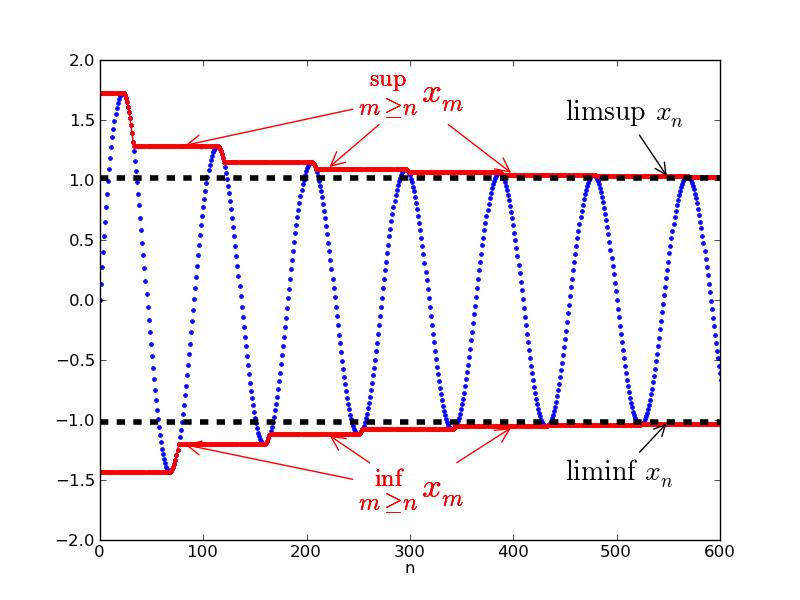
\includegraphics[width=\textwidth]{Lim_sup_example_5}
\begin{Definition}
	A number (or the symbol $ - \infty $ or $ +\infty $) is called a \textit{partial limit} of a sequence, if the sequence contains a subsequence converging to that number.
\end{Definition}

\begin{Proposition}
	The inferior and superior limits of any sequence are respectively the smallest and largest partial limits of the sequence.
\end{Proposition}
\begin{proof}
	Let's assume that this sequence is bounded. First consider the inferior limit $ i = \varliminf_{k \to \infty}x_k $. The sequence $ i_n = \inf_{k\geqslant n}x_k $ is nondecreasing. Using the definition of the greatest lower bound, we choose by induction numbers $ k_n \in \Natural $ such that $ k_n < k_{n+1} $ and $ i_{k_n} \leqslant x_{k_n} < i_{k_n}+\frac{1}{n} $ (Taking $ i_1 $ we find $ k_1 $; taking $ i_{k_1+1} $ we find $ k_2 $, etc.). Since $ \lim\limits_{n \to \infty}i_n = \lim\limits_{n \to \infty}(i_n+\frac{1}{n}) = i $, we have $ \lim\limits_{n \to \infty}x_{k_n}=i $. It is the smallest partial limit since for every $ \varepsilon>0 $ there exists $ n \in \Natural $ such that $ i-\varepsilon<i_n $, that is $ i-\varepsilon <i_n = \inf_{k\geqslant n}x_k \leqslant x_k $ for any $ k \geqslant n $. Now we have $ i-\varepsilon < x_k $ for $ k >n $ means that no partial limit of the sequence can be less than $ i - \varepsilon $. But $ \varepsilon >0 $ is arbitrary, and hence no partial limit can be less than $ i $. The proof for the superior limit is of course analogous. \newpara
	Now if the sequence is not bounded below(resp. above), one can select a subsequence of it tending to $ -\infty $ (resp. $ +\infty $). But then we also have $ \varliminf_{k \to \infty}x_k = -\infty $ (resp. $ \varlimsup_{k \to \infty}x_k = +\infty $). Finally, if $ \varlimsup_{k \to \infty}x_k = -\infty $ (resp. $ \varliminf_{k \to \infty}x_k = +\infty $), the sequence itself tends to $ -\infty $ (resp. $ +\infty $).
\end{proof}

\begin{Corollary}
	A sequence has a limit or tends to $ \pm \infty $ iff its inferior and superior limits are the same.
\end{Corollary}
\begin{proof}
	The cases when $ \varliminf_{k \to \infty}x_k = \varlimsup_{k \to \infty}x_k = \pm \infty $ have benn investigated above, and so we may assume that $ \varliminf_{k \to \infty}x_k = \varlimsup_{k \to \infty}x_k = A \in \Real $. Since $ (i_n = \inf_{k \geqslant n}x_k) \leqslant x_k \leqslant (\sup_{k \geqslant n}x_k = s_n) $, we have $ \lim\limits_{n \to \infty}x_n = A $.
\end{proof}

\begin{Corollary}
	A sequence converges iff every subsequence of it converges.
\end{Corollary}
\begin{proof}
	The inferior and superior limits of a subsequence lie between those of the sequence itself. If the sequence converges, then its subsequences must converge, and their limits are the same. The converse assertion is obvious, since the subsequence can be chosen as the sequence itself.
\end{proof}

\begin{Corollary}
	The Bolzano-Weierstrass Lemma in its restricted and wider formulations(corresponding to Lemmas at page 32 and page 33) follows from the Proposition we just proved.
\end{Corollary}
\begin{proof}
	If the sequence $ \{x_k\} $ is bounded, then $ i = \varliminf_{k \to \infty}x_k $ and $ s = \varlimsup_{k \to \infty}x_k $ are finite and partial limits of the sequence. When $ i=s $ some subsequences have a unique limit, and at least two when $ i<s $. If the sequence is unbounded on one side or the other, there exists a subsequence tending to the corresponding infinity.
\end{proof}



\subsection{Elementary Facts about Series}

\subsubsection{The Sum of a Series and the Cauchy Criterion for Convergence of Series}

\begin{Definition}
	The expression $ a_1 + a_2 + \cdots +a_n + \cdots$ is denoted by the symbol $ \sum_{n=1}^{\infty}a_n $ and usually called a \textit{series} or an \textit{infinite series}.
\end{Definition}

\begin{Definition}
	The elements of the sequence $ \{a_n\} $, when regarded as elements of the series, are called the \textit{terms} of the series. The element $ a_n $ is called the \textit{$ n $th term}.
\end{Definition}

\begin{Definition}
	The sum $ s_n = \sum_{k=1}^{n}a_k $ is called the \textit{partial sum of the series} or the \textit{$ n $th partial sum of the series}.
\end{Definition}

\begin{Definition}
	If the sequence $ \{s_n\} $ of partial sums of a series converges(resp. divergence), we say the series is \textit{convergent} (resp. \textit{divergent}).
\end{Definition}

\begin{Definition}
	The limit $ \lim\limits_{n \to \infty}s_n = s $ of the sequence of partial sums of the series, if it exists, is called the \textit{sum of the series}.
\end{Definition}
One can see that $ \sum_{n=1}^{\infty}a_n=s $.

\begin{Theorem}[The Cauchy convergence criterion for a series]
	The series $ a_1 + \cdots + a_n + \cdots $ converges iff for every $ \varepsilon >0 $ there exists $ N \in \Natural $ such that the inequalities $ m \geqslant n > N $ imply $ |a_n + \cdots +a_m|<\varepsilon $.
\end{Theorem}

\begin{Corollary}
	If only a finite number of terms of a series are changed, the resulting new series will converge if the original series did and diverge if it diverged.
\end{Corollary}

\begin{Corollary}
	A necessary condition for convergence of the series $ a_1 + \cdots + a_n + \cdots $ is that the terms tend to zero as $ n \to \infty $, that is, it is necessary that $ \lim\limits_{n \to \infty}a_n=0 $.
\end{Corollary}
\begin{proof}
	Set $ m=n $ in the Cauchy convergence criterion and use the definition of the limit of a sequence. \newpara
	Alternatively, $ a_n = s_n - s_{n-1} $, and, given that $ \lim\limits_{n \to \infty}s_n=s $, we have $ \lim\limits_{n \to \infty} a_n =  \lim\limits_{n \to \infty} (s_n - s_{n-1}) = s -s = 0$ .
\end{proof}

\begin{Example}
	The series $ 1+q+q^2+ \cdots + q^n + \cdots  $ is often called the \textit{geometric series}. It converges iff $ |q|<1 $.
\end{Example}
\begin{proof}
	Suppose $ |q|\geqslant 1 $, then we have $ |q^n| \geqslant 1 $, and in this case this series does not converges.\newpara
	Now let $ |q|<1 $, and we'll have $ s_n = 1+ q + \cdots + q^{n-1} = \frac{1-q^n}{1-q} $ and $ \lim\limits_{n \to \infty}s_n = \frac{1}{1-q} $, since $ \lim\limits_{n \to \infty}q^n = 0 $ if $ |q|<1 $.
\end{proof}

\begin{Example}
	The series $ 1+\frac{1}{2}+ \cdots +\frac{1}{n}+ \cdots$, called the \textit{harmonic series}, diverges because its partial sums $ s_n = 1+ \frac{1}{2}+\cdots \frac{1}{n} $ diverges.
\end{Example}
\begin{proof}
	It's sufficient to prove that its partial sum $ s_n = 1+ \frac{1}{2}+\cdots \frac{1}{n} $ diverges. For all $ n \in \Natural $ we have 
	\begin{equation}
		|x_{2n}-x_n| = \frac{1}{n+1}+ \cdots + \frac{1}{n+n} > n \cdot \frac{1}{2n} = \frac{1}{2}\nonumber
	\end{equation}
	and our proof completes.
\end{proof}

\textbf{\textit{Remark}} Usual laws for dealing with finite sums does not apply to series in general (e.g. insert parentheses to a divergent series). 

\subsubsection{Absolute Convergence. The Comparison Theorem and Its Consequences}

\begin{Definition}
	The series $ \sum_{n=1}^{\infty} $ is \textit{absolutely} convergent if the series $ \sum_{n=1}^{\infty}|a_n| $ converges.
\end{Definition}

Since $ |a_n + \cdots + a_m| \leqslant |a_n|+\cdots |a_m|$, the Cauchy convergence criterion implies that an absolutely convergent series converges, but the converse is generally not true.

\begin{Example}
	The series $ 1-1+\frac{1}{2}-\frac{1}{2}+ \frac{1}{3}-\frac{1}{3}+ \cdots$, whose partial sums are either $ \frac{1}{n} $ or $ 0 $, converges to $ 0 $. However, this sequence does not absolutely converges, and its proof is similar to the proof for the divergence of harmonic series.
\end{Example}

\begin{Theorem}[Criterion for convergence of series of non-negative terms]
	A series whose terms are non-negative converges iff the sequence of partial sums is bounded above.
\end{Theorem}

\begin{Theorem}[Comparison Theorem]
	Let $ \sum_{n=1}^{\infty}a_n $ and $ \sum_{n=1}^{\infty}b_n $ be two series with non-negative terms. If there exists an index $ N\in \Natural $ such that $ a_n \leqslant b_n $ for all $ n >N $, then the convergence of the series $  \sum_{n=1}^{\infty}b_n $ implies the convergence of $ \sum_{n=1}^{\infty}a_n $, and the divergence of $ \sum_{n=1}^{\infty}a_n $ implies the divergence of $\sum_{n=1}^{\infty}b_n $.
\end{Theorem}
\begin{proof}
	Omit terms for these two series for all $ n < N $, since a finite number of terms has no effect on the convergence of a series. Denote the partial sum of the sequences as $ A_n = \sum_{k=1}^{n}a_k \leqslant \sum_{k=1}^{n}b_k=B_n $. If the series $ \{B_n\} $ converges, then $ \{A_n\} $ is bounded above. Because $ \{A_n\} $ is also non-decreasing (all terms are non-negative), it has a limit, and so do $  \sum_{n=1}^{\infty}a_n  $. The second assertion is similar and can be proved by contradiction.
\end{proof}

\begin{Corollary}[The Weierstrass M-test for absolute convergence]
		Let $ \sum_{n=1}^{\infty}a_n $ and $ \sum_{n=1}^{\infty}b_n $ be series. Suppose there exists an index $ X $ such that $ |a_n| \leqslant b_n $ for all $ n > N $. Then a sufficient condition for absolute convergence of the series $ \sum_{n=1}^{\infty}a_n $ is that the series $ \sum_{n=1}^{\infty}b_n $ converge. \newpara
		It's often summarized as following: I\textbf{f the terms of a series are majorized (in absolute value) by the terms of a convergent numerical series, then the original series converges absolutely}.
\end{Corollary}
\begin{proof}
	By the comparison theorem the series $ \sum_{n=1}^{\infty}|a_n| $ will then converge, and that is what is meant by the absolute convergence of $ \sum_{n=1}^{\infty}a_n $.
\end{proof}

\begin{Corollary}[Cauchy's Test]
	Let $ \sum_{n=1}^{\infty}a_n $ be a given series and $ \alpha = \varlimsup_{n \to \infty} \sqrt[n]{|a_n|}$. Then the following are true:\\
	a) if $ \alpha <1 $, the series converges absolutely;\\
	b) if $ \alpha >1 $, the series diverges; \\
	c) there exist both absolutely convergent and divergent series for which $ \alpha = 1 $.
\end{Corollary}
\begin{proof}
	For $ \alpha>0 $, we find a $ q \in \Real $ such that $ \alpha <q<1 $, and show that the sequence $ \sum_{n=1}^{\infty}q^n $ converges and its terms are always greater than $ |a_n| $. Thus the original sequence absolutely converges. \newpara
	For $ \alpha>1 $, we find that $ \alpha $ is the greatest partial limit of the sequence $ \{\sqrt[n]{|a_n|}\} $. Hence for some $ k>K (|a_{n_k}|>1)  $, and the necessary condition for convergence ($ a_n \to 0 $) does not meet for the original sequence. \newpara
	If $ \alpha=1 $, for example, the series $ \sum_{n=1}^{\infty}\frac{1}{n} $ diverges and $ \sum_{n=1}^{\infty}\frac{1}{n^2} $ converges absolutely, but their superior limit under $ n $th root are both $ 1 $.
\end{proof}

\begin{Corollary}[d'Alembert's Test]
	Suppose the limit $ \lim\limits_{n \to \infty} |\frac{a_{n+1}}{a_n}|= \alpha $ exists for the series $ \sum_{n=1}^{\infty}a_n $. Then, \\
	a) if $ \alpha <1 $, the series converges absolutely;\\
	b) if $ \alpha >1 $, the series diverges; \\
	c) there exist both absolutely convergent and divergent series for which $ \alpha = 1 $.
\end{Corollary}

\begin{proof}
	If $ \alpha<1 $, then we find a number $ q $ such that $ \alpha < q <1 $. Fixing $ q $ and use the properties of limits, we find an index $ N \in \Natural$ such that $ |\frac{a_{n+1}}{a_n}|<q $ for $ n > N $. Since
	\begin{equation}
		|\frac{a_{n+1}}{a_n}|\cdot |\frac{a_n}{a_{n-1}}|\cdots |\frac{a_2}{a_1}| = \frac{a_{n+1}}{a_1}\nonumber
	\end{equation}
	and therefore we have $ |a_{n+1}|<|a_1|\cdot q^n $. But the geometric series $ \sum_{n=1}^{\infty}|a_1|q^n $ converges for $ |q|<1 $, hence the original series converges. \newpara
	For $ \alpha >1 $, we can find some terms that $ |\frac{a_{n+1}}{a_n}|>1 $, thus it diverges. For case involving $ \alpha=1 $, the examples from our proof for \textbf{Cauchy's Test} are sufficient.
\end{proof}

\begin{Proposition}[Cauchy]
	If $ a_1 \geqslant a_2 \geqslant \cdots \geqslant 0 $, the series $ \sum_{n=1}^{\infty}a_n $ converges iff the series $ \sum_{k=0}^{\infty}2^ka_{2^k} = a_1 + 2a_2 + 4a_4 + 8a_8 \cdots$ converges.
\end{Proposition}
\begin{proof}
	By the inequality
	\begin{equation}
		2^na_{2^{n+1}} \leqslant a_{2^n+1} + \cdots + a_{2^{n+1}} \leqslant 2^na_{2^n}
	\end{equation}
	we have 
	\begin{equation}
		\frac{1}{2}(S_{n+1}-a_1)\leqslant A_{2^{n+1}}-a_1 \leqslant S_n
	\end{equation}
	where $ A_k = a_1 + \cdots +a_k $ and $ S_n = a_1+2a_2+\cdots +2^n a_{2^n} $. $ \{A_k\} $ and $ \{S_n\} $ are non-decreasing, and hence they are both bounded above or unbounded above. Since all their terms are non-negative, our proof completes.
\end{proof}

\begin{Corollary}
	The series $ \sum_{n=1}^{\infty}\frac{1}{n^p} $ converges for $ p>1 $ and diverges for $ p \leqslant1 $.
\end{Corollary}
\begin{proof}
	If $ p \geqslant0 $, by our proposition it converges when $ 2^{1-p}<1 $, that is, $ p>1 $. The case when $ p \leqslant 0 $ is obvious since all terms are not smaller than 1.
\end{proof}


\subsubsection{The Number $ e $ as the Sum of a Series}
We know that $ e=\lim\limits_{n \to \infty}(1+\frac{1}{n})^n $. By Newton's binomial formula:
\begin{align}
	(1+\frac{1}{n})^n &= 1 + \frac{n}{1!}\frac{1}{n} + \frac{n(n-1)}{2!}\frac{1}{n^2} + \cdots + \frac{(n(n-1)\cdots(n-k+1))}{k!}\frac{1}{n^k}+ \cdots +\frac{1}{n^n} \\
	&= 1+ 1+ \frac{1}{2!}(1-\frac{1}{n}) + \cdots + \frac{1}{k!}(1-\frac{1}{n})(1-\frac{2}{n}) \times \cdots \\
	&\times (1-\frac{k-1}{n}) + \cdots + \frac{1}{n!}(1-\frac{1}{n})\cdots(1-\frac{n-1}{n})
\end{align}
Setting $ (1+\frac{1}{n})=e_n $ and $ 1+1+\cdots \frac{1}{2!} + \cdots + \frac{1}{n!}=s_n$, we thus have $\forall n \in \Natural(e_n < s_n)  $. \newpara
On the other hand, for any fixed $ k $ and $ n \geqslant k $, as can be seen from the same expansion, we have
\begin{equation}
	1+1+1+ 1+ \frac{1}{2!}(1-\frac{1}{n}) + \cdots + \frac{1}{k!}(1-\frac{1}{n})(1-\frac{2}{n})\cdots (1-\frac{k-1}{n})<e_n \nonumber
\end{equation}
As $ n \to \infty $ the left-hand side of the inequality tends to $ s_k $ and the right-hand side to $ e $. We can now conclude that $ s_k \leqslant e $ for all $ k \in \Natural $. Then from the relation $ e_n < s_n \leqslant e $ we find that $ \lim\limits_{n \to \infty}s_n=e $.
\begin{Definition}
	$ e=1+\frac{1}{1!}+ \frac{1}{2!}+\cdots+\frac{1}{n!}+\cdots $
\end{Definition}
The difference between $ e $ and its estimation $ s_n $ can be expressed as following
\begin{align}
	0<e-s_n &= \frac{1}{(n+1)!}+ \frac{1}{(n+2)!}+ \cdots =\\
	&= \frac{1}{(n+1)!}[1+\frac{1}{n+2}+\frac{1}{(n+2)(n+3)}+\cdots] < \\
	&< \frac{1}{(n+1)!}[1+\frac{1}{n+2}+\frac{1}{(n+2)^2}+\cdots] \\
	&=\frac{1}{(n+1)!}\frac{1}{1-\frac{1}{n+2}} = \frac{n+2}{n!(n+1)^2} < \frac{1}{n!n}
\end{align}
This estimate of the difference $ e-s_n $ can be written as the equality 
\begin{equation}
	e=s_n+\frac{\theta_n}{n!n} \nonumber
\end{equation}

where $ 0<\theta_n<1 $. \\

Hence $ e $ is irrational.
\begin{proof}[$ e $'s irrationality]
	Suppose the contrary, that $ e = \frac{p}{q} $, where $ p,q \in \Natural $. Then the number $ q!e $ must be an integer, while
	\begin{equation}
		q!e = q!(s_q+\frac{\theta_n}{q!q}) = q!+\frac{q!}{1!}+ \frac{q!}{2!}+\cdots+\frac{q!}{n!}+\frac{\theta_q}{q} \nonumber
	\end{equation}
	and therefore $ \frac{\theta_q}{q} $ would have to be an integer, which is impossible.
\end{proof}

Moreover, $ e $ is transcendental.





\section{The Limit of a Function}

\subsection{Definitions and Examples}

	Let $ E \subset \Real $, $ a $ be an limit point of $ E $, and $ f : E \to \Real $ be a real-valued function defined on $ E $.
\begin{Definition}
The function $ f : E \to \Real  $ \textit{tends to} $ A $ as $ x $ \textit{tends to} $ a $, or that $ A $ is the \textit{limit} of $ f $ as $ x $ \textit{tends to} $ a $, if for every $ \varepsilon>0 $ there exists $ \delta>0 $ such that $ |f(x)-A|<\varepsilon $ for every $ x \in E $ such that $ 0<|x-a|<\delta $.
\begin{equation}
	\forall \varepsilon >0 \exists \delta >0 \forall x \in E(0<|x-a|<\delta \Rightarrow |f(x)-A|<\varepsilon)\nonumber
\end{equation}
which is denoted as $ \lim\limits_{E \ni x \to a}f(x) = A $.
\end{Definition}

\begin{Example}
	\begin{equation}
		\lim\limits_{E \ni x \to 0}x\sin\frac{1}{x}=0\nonumber
	\end{equation}
	\begin{proof}
		Let $ \varepsilon=\delta $.
	\end{proof}
\end{Example}

\begin{Definition}
	A \textit{deleted neighborhood} of a point is a neighborhood of the point from which the point itself has been removed. \newpara
	If $ U(a) $ denotes a neighborhood of $ a $, the deleted neighborhood is denoted as $ \mathring{U}(a) $. \newpara
	The sets
	\begin{align}
		U_E(a) &\coloneqq E \cap U(a) \\
		\mathring{U}_E(a)&\coloneqq E \cap \mathring{U}(a)
	\end{align}
	will be called respectively a \textit{neighborhood of $ a $} in $ E $ and a \textit{deleted neighborhood of $ a $} in $ E $. \newpara
	if the temporarily-adopted cumbersome symbols $ \mathring{U}^\delta_E(a) $ and $ V^\varepsilon _\Real(A) $ denote the deleted $ \delta $-neighborhood of $ a $ in $ E $ and the $ \varepsilon $-neighborhood of $ A $ in $ \Real $, then the definition of the limit of a function can be rewritten as
	\begin{equation}
		(\lim\limits_{E \ni x \to a}f(x) = A ) \coloneqq \forall V^\varepsilon_\Real(A)\exists\mathring{U}^\delta_E(a)(f(\mathring{U}^\delta_E(a))\subset V^\varepsilon_\Real(A)) .\nonumber
	\end{equation}
	This expression says that $ A $ is the limit of the function $ f $ as $ x $ tends to $ a $ in the set $ E $ if for every $ \varepsilon $-neighborhood $ V^\varepsilon_\Real(A) $ of $ A $ there exists a deleted $ \delta $-neighborhood $ \mathring{U}^\delta_E(a) $ of $ a $ in $ E $ whose image $ f(\mathring{U}^\delta_E(a)) $ under the mapping $ f:E\to \Real $ is entirely contained in $  V^\varepsilon_\Real(A) $.
\end{Definition}
Since every neighborhood of a point on the real line contains a symmetric neighborhood (a $ \delta $-neighborhood) of the same point, the \textbf{final version of our definition for a limit} is:
\begin{Definition}
	\begin{equation}
			(\lim\limits_{E \ni x \to a}f(x) = A ) \coloneqq \forall V_\Real(A)\exists\mathring{U}_E(a)(f(\mathring{U}_E(a))\subset V_\Real(A)) .\nonumber
	\end{equation}
\end{Definition}

\begin{Example}
	The function \begin{equation}
	sgn x =	\begin{cases} 1 & \text{for } x >0\\
		 0 & \text{for } x=0\\
		 -1 & \text{for } x<0
		 \end{cases} \nonumber
	\end{equation}
	(read "signum x") has no limit as $ x \to 0 $.
\end{Example}
\begin{proof}
Apparently no number distinct from $ -1,0,1 $ can be the limit of the function.But no matter what $ \mathring{U}(0) $ we choose, some points of it does not belong to the $ \varepsilon $-neighborhood of $ A $ with $ \varepsilon=\frac{1}{2} $, since $  \mathring{U}(0)  $ contains both positive and negative points while $ V(A) $ can't contain both $ 1 $ and $ -1 $ at the same time.
\end{proof}
When the function $ f $ is defined on a whole deleted neighborhood of a point $ a\in \Real $, that is, when $ \mathring{U}_E(a)=\mathring{U}_\Real(a)=\mathring{U}(a) $, we adopt the expression $ x \to a $ instead of $ E \ni x \to a $.

\begin{Example}
	\begin{equation}
		\lim\limits_{x \to 0} |sgn(x)|=1\nonumber
	\end{equation}
\end{Example}
\begin{proof}
	\begin{equation}
		\forall V(1) (f(\mathring{U}(0))=1\in V(1)) \nonumber
	\end{equation}
\end{proof}

\begin{Example}
	\begin{equation}
		\lim\limits_{\Real_-\ni x \to 0} sgn(x)=-1, \quad 	\lim\limits_{\Real_+\ni x \to 0} sgn(x)=1 \nonumber
	\end{equation}
\end{Example}

\begin{Example}
	$ \lim\limits_{x \to 0}\sin \frac{1}{x} $ has no limit.
\end{Example}
\begin{proof}
	In any deleted neighborhood of 0 $ \mathring{U}(0) $ there are always points of the form $ \frac{1}{-\pi/2+2\pi n} $ and $  \frac{1}{\pi/2+2\pi n} $ which assume the values $ -1 $ and $ 1 $ respectively, but for $ \varepsilon<1 $ these two numbers can't both lie in the $ \varepsilon $-neighborhood. 
\end{proof}

\begin{Example}
	If 
	\begin{align}
		E_- &=\{x\in \Real | x = \frac{1}{-\pi/2+2\pi n}, n \in \Natural\} \\
		E_+ &=\{x\in \Real | x = \frac{1}{\pi/2+2\pi n}, n \in \Natural\}
	\end{align}
	then
	\begin{align}
		&\lim\limits_{E_-\ni x \to 0}\sin \frac{1}{x} = -1 \\
		&\lim\limits_{E_+\ni x \to 0}\sin \frac{1}{x} = 1
	\end{align}
\end{Example}
The next proposition, also called the statement of the equivalence of the Cauchy definition of a limit(in terms of neighborhoods) and the Heine definition(in terms of sequences), is:
\begin{Proposition}
	The relation $ \lim\limits_{E \ni x \to a}f(x) = A $ holds iff for every sequence $ \{x_n\} $ of points $ x_n \in E\setminus a $ converging to $ a $, the sequence $ \{f(x_n)\} $ converges to $ A $.
\end{Proposition}
\begin{proof}
	First, $ (\lim\limits_{E \ni x \to a}f(x)=A) \Rightarrow(\lim\limits_{n \to \infty}f(x_n)=A) $ is obvious. Now for the converse, if $ A $ is not the limit of $ f(x) $ as $ E \ni x \to a $, then there exists a neighborhood $ V(A) $ such that for any $ n \in \Natural $, there is a point $ x_n $ in the deleted $ \frac{1}{n} $-neighborhood of $ a $ in $ E $ such that $ f(x_n)\notin V(A) $. But this means that the sequence $ \{f(x_n)\} $ does not converge to $ A $.
\end{proof}













\subsection{Properties of the Limit of a Function}

\subsubsection{Properties of Deleted Neighborhood of a Limit Point of a Set }
\begin{Example}
	$ \mathring{U}_E(a)\neq \varnothing $, that is, the deleted neighborhood of the point in $ E $ is nonempty.
\end{Example}
\begin{Example}
	$ \forall \mathring{U}^\prime_E(a)\forall \mathring{U}^{\prime\prime}_E(a)\exists\mathring{U}_E(a)(\mathring{U}_E(a)\subset \mathring{U}^\prime_E(a) \cap \mathring{U}^{\prime\prime}_E(a)) $, that is, the intersection of any pair of deleted neighborhoods contains a deleted neighborhood.
\end{Example}

\subsubsection{General Properties of the Limit of a Function}
\begin{Definition}
	A function $ f : E \to \Real $ assuming only one value is called \textit{constant}. A function $ f : E \to \Real  $ is called \textit{ultimately constant} as $ E \ni x \to a $ if it is constant in some deleted neighborhood $ \mathring{U}_E(a) $, where $ a $ is a limit point of $ E $.
\end{Definition}
\begin{Definition}
	A function $ f : E \to \Real  $ is \textit{bounded, bounded above,} or \textit{bounded below} respectively if there is a number $ C \in \Real $ such that $ |f(x)|<C $, $ f(x)<C $, or $ C<f(x) $ for all $ x \in E $.
\end{Definition}

\begin{Theorem}
	\textbf{a)} ($ f : E \to \Real  $ is ultimately the constant $ A $ as $ E \ni x \to a) \Rightarrow  (\lim\limits_{E \ni x \to a}f(x)=A)$ . \newpara
	\textbf{b)} $ (\exists \lim\limits_{E \ni x \to a}f(x))\Rightarrow (f: E \to \Real\text{ is ultimately bounded as } E \ni x \to a )$. \newpara
	\textbf{c)} $ (\lim\limits_{E \ni x \to a}f(x)=A_1 )\land(\lim\limits_{E \ni x \to a}f(x)=A_2 )\Rightarrow (A_1=A_2)$.
\end{Theorem}
\begin{proof}
	The proof is similar to how we prove that a ultimately constant sequence converges and its limits is unique.
\end{proof}

\subsubsection{Passage to the Limit and Arithmetic Operations}
\begin{Definition}
	If two numerical-valued functions $ f: E \to \Real $ and $ g : E \to \Real $ have a common domain of definition $ E $, the \textit{sum, product}, and \textit{quotient} are respectively the functions defined on the same set by the following formulas
	\begin{align}
		(f+g)(x)&\coloneqq f(x) + g(x) \\
		(f \cdot g)(x)&\coloneqq f(x)\cdot g(x)\\
		(\frac{f}{g})(x) &\coloneqq \frac{f(x)}{g(x)}\text{ if }\forall x \in E (g(x) \neq 0)  \\
	\end{align}
\end{Definition}


\begin{Definition}
	A function $ f : E \to \Real $ is said to be \textit{infinitesimal} as $ E \ni x \to a $ if $ \lim\limits_{E \ni x \to a}f(x)=0 $.
\end{Definition}

\begin{Proposition}
	\textbf{a)} If $ \alpha : E \to \Real $ and $ \beta : E \to \Real $ are infinitesimal functions as $ E \ni x \to a $, then their sum $ \alpha + \beta: E \to \Real $ is also infinitesimal as $ E \ni x \to a $. \newpara
	\textbf{b)} If $ \alpha : E \to \Real $ and $ \beta : E \to \Real $ are infinitesimal functions as $ E \ni x \to a $, then their product $ \alpha \cdot \beta: E \to \Real $ is also infinitesimal as $ E \ni x \to a $. \newpara
	\textbf{c)}  If $ \alpha : E \to \Real $ is infinitesimal as $ E \ni x \to a $ and $ \beta : E \to \Real $ is ultimately bounded as $ E \ni x \to a $, then the product $ \alpha \cdot \beta: E \to \Real $ is infinitesimal as $ E \ni x \to a $.
\end{Proposition}
\begin{proof}
	For assertion \textbf{a)}, we set $ |\alpha(x)<\frac{\varepsilon}{2}| $. \\
	Assertion \textbf{b)} is a special case of assertion \textbf{c)}, since every function that has a limit is ultimately bounded. \\
	Let $ M $ bounds $ |\beta(x)| $, and set $ |\alpha(x)| < \frac{\varepsilon}{M} $ will help to prove assertion \textbf{c)}.
\end{proof}

\begin{Example}
	\begin{equation}
	(\lim\limits_{E \ni x \to a}f(x)=A) \Leftrightarrow (f(x)=A+\alpha(x)\land \lim\limits_{E \ni x \to a} \alpha(x)=0) \nonumber
	\end{equation}
\end{Example}
\begin{proof}
	This follows immediately from the definition of limit, by virtue which
	\begin{equation}
	\lim\limits_{E \ni x \to a}f(x)=A \Leftrightarrow \lim\limits_{E \ni x \to a}(f(x)-A)=0 \nonumber
	\end{equation}
\end{proof}

\begin{Theorem}
	Let $ f: E \to \Real $ and $ g : E \to \Real $ be two functions with a common domain of definition. If $ \lim\limits_{E \ni x \to a}f(x)=A $ and $  \lim\limits_{E \ni x \to a}g(x)=B  $, then
	\begin{align}
		&\lim\limits_{E \ni x \to a}(f+g)(x)= A+B \\
		&\lim\limits_{E \ni x \to a}(f \cdot g)(x)= A \cdot B\\
		&\lim\limits_{E \ni x \to a}(\frac{f}{g})(x) = \frac{A}{B}\text{ if }\forall x \in E (g(x) \neq 0\text{ and }B \neq 0)  \\
	\end{align}
\end{Theorem}
\begin{proof}
	These properties can be derived from the properties of the limit of sequences according to the proposition above. In order to complete the proof, one only need to convert "for some $ N \in \Natural $" to $ \mathring{U}_E(a) $.
\end{proof}
\begin{proof}[alternative proof with infinitesimal functions]
	Let $ f(x)= \alpha(x)$ and $ g(x)=\beta(x) $, where $ \alpha(x) $ and $ \beta(x) $ are infinitesimal functions. The first two assertions are obvious. For the quotient one, find the value of $ \frac{f(x)}{g(x)}-\frac{A}{B} $ after proving that $ \frac{1}{g(x)} $ is ultimately bounded as $ E \ni x \to a $.
\end{proof}

\subsubsection{Passage to the Limit and Inequalities}
\begin{Theorem}
	\textbf{a)} If the functions $ f : E \to \Real $ and $ g: E \to \Real $ are such that $ \lim\limits_{E \ni x \to a}f(x)=A $, and $ \lim\limits_{E \ni x \to a}g(x)=B $ and $ A <B $, then there exists a deleted neighborhood $ \mathring{U}_E(a) $ of $ a $ in $ E $ at each point of which $ f(x)<g(x) $. \newpara
	\textbf{b)} If the relations $ f(x) \leqslant g(x) \leqslant h(x) $ hold for the functions $ f : E \to \Real $, $ g: E \to \Real $ and $ h:E \to \Real $, and if $  \lim\limits_{E \ni x \to a}f(x)= \lim\limits_{E \ni x \to a}h(x)=C $, then the limit of $ g(x) $ exists as $ E \ni x \to a $, and $ \lim\limits_{E \ni x \to a}g(x)=C $.
\end{Theorem}
\begin{proof}
	\textbf{a)} Choose a number $ C $ such that $ A<C<B $. By definition of limit, we find deleted neighborhoods $ \mathring{U}^\prime_E(a) $ and $ \mathring{U}^{\prime\prime}_E(a)  $ such that $ |f(x)-A|<C-A $ for $ x \in \mathring{U}^\prime_E(a)  $ and $ |g(x)-B|<B-C$ for $ x \in  \mathring{U}^{\prime\prime}_E(a)$. Then at any point of a deleted neighborhood $ \mathring{U}_E(a) $ contained in $ \mathring{U}^\prime_E(a) \cup  \mathring{U}^{\prime\prime}_E(a)  $, we have 
	\begin{equation}
		f(x)<A+(C-A) =C = B-(B-C)<g(x) \nonumber
	\end{equation}
	\textbf{b)} This proof is similar.
\end{proof}

\begin{Corollary}
	Suppose $ \lim\limits_{E \ni x \to a}f(x)=A $ and $ \lim\limits_{E \ni x \to a}g(x)=B $ . Let $ \mathring{U}_E(a) $ be a deleted neighborhood of $ a $ in $ E $. \newpara
	\textbf{a)} If $ f(x) > g(x) $ for all $ x \in  \mathring{U}_E(a)$, then $ A \geqslant B $; \newpara
	\textbf{b)} $ f(x) \geqslant g(x) $ for all $ x \in  \mathring{U}_E(a)$, then $ A \geqslant B $; \newpara
	\textbf{c)} $ f(x) > B $ for all $ x \in  \mathring{U}_E(a)$, then $ A \geqslant B $; \newpara
	\textbf{d)} $ f(x) \geqslant B $ for all $ x \in  \mathring{U}_E(a)$, then $ A \geqslant B $.
\end{Corollary}
\begin{proof}
	Assertion a) and b) can be proved by contradiction and the theorem mentioned above. Set $ g(x) \equiv B $ and we prove assertion c) and d).
\end{proof}

\subsubsection{Two Important Examples}
\begin{Example}
	\begin{equation}
		\lim\limits_{x \to 0}\frac{\sin x}{x}=1 \nonumber
	\end{equation}
\end{Example}
\begin{proof}
	The geometric proof is sufficient with the following conditions:
	\begin{align}
		&|\sin x| \leqslant |x| \nonumber \\
		& 0\leqslant |\sin x| \leqslant |x| \Rightarrow (\lim\limits_{x \to 0} |\sin x| = 0) \nonumber
	\end{align}
\end{proof}

Now we define the exponential, logarithmic, and power functions using the theory of real numbers and limits.
\textbf{A)} \textit{The exponential function} \newpara
Let $ a>1 $ \\
$ 1^0 $ For $ n \in \Natural $ we define inductively $ a^1 \coloneqq a\text{ , } a^{n+1} \coloneqq a^n \cdot a $\newpara
$ 2^0 $ $ a^0 = 1 \text{ , } a^{-n}=\frac{1}{a^n} $ \newpara
$ 3^0 $ We define $ a = a^1 = (a^{1/n})^m $ and $ a^{m/n} \coloneqq (a^{1/n})^m $, Now we have defined $ a^r $ for $ r \in \Quoziente $. \newpara
$ 4^0 $ By induction, for $ x>0 $ and $ y>0 $ we have $ (x<y) \Leftrightarrow (x^n<y^n) $, and in particular, $ (x=y)\Leftrightarrow (x^n = y^n) $.\newpara
$ 5^0 $ $ a^{(mk)/(nk)} = a^{m/n} $ for $ k \in \Zahlen $ and $ a^{m_1/n_1}\cdot  a^{m_2/n_2}=a^{m_1/n_1+m_2/n_2} $\newpara
$ 6^0 $ $ (r_1<r_2)\Rightarrow (a^{r_1}<a^{r_2}) $ for any $ r_1,r_2\in\Quoziente $.\newpara
$ 7^0 $ For $ r^0 \in \Quoziente (\lim\limits_{\Quoziente \ni r \to r_0}a^r=a^{r_0})$.
\begin{proof}
	First we prove that $ a^p\to1 $ as $ \Quoziente \ni p \to 0 $ by use the inequality $ a^{-1/n}<a^p<a^{1/n} $. Then we choose $ \delta $ such that $ 1-\varepsilon a^{-r_0} <a^p < 1 + \varepsilon a^{-r_0}$ for $ |p|<\delta $. If now $ |r-r_0|<\delta $, we have $ a^{r_0}(1-\varepsilon a^{-r_0} )<a^{r_0}\cdot a^{r-r_0} < a^{r_0}(1 + \varepsilon a^{-r_0} )$, which says $ a^{r_0}- \varepsilon < a^r< a^{r_0}+ \varepsilon$.
\end{proof}
$ 8^0 $ Let $ x \in \Real $, $ s = \sup_{\Quoziente \ni r <x}a^r $, and $ i = inf_{\Quoziente \ni r >x}a^r  $. We show that $ s=i $.
\begin{proof}
	\begin{equation}
		a^{r_1}\leqslant s \leqslant i \leqslant a^{r_2}\nonumber
	\end{equation}
	and for $ 0<|r_2-r_1|<\delta $ we have $ 0 \leqslant i-s \leqslant\varepsilon $.
\end{proof}
We now define $ a^x \coloneqq s = i $. \newpara
$ 9^0 $ $ a^x = \lim\limits_{\Quoziente \ni r \to x}a^r $.
\begin{proof}
	We find $ r^\prime <x $ such that $ s - \varepsilon < a^{r^\prime} \leqslant s = a^x $ and $ r^{\prime\prime}>x $ such that $ a^x = i \leqslant a^{r^{\prime\prime} }< i+ \varepsilon$. Then for all $ r \in \Quoziente $ in $ (r^{\prime},r^{\prime\prime}) $
	\begin{equation}
		a^x - \varepsilon < a^r < a^x + \varepsilon \nonumber
	\end{equation}
\end{proof}
$ 10^0 $ For $ x_1,x_2 \in \Real $ and $ a >1 $, $ (x_1<x_2)\Rightarrow (a^{x_1}<a^{x_2}) $.\newpara
$ 11^0 $ For any $ x_1,x_2 \in \Real $, $ a^{x_1}\cdot a^{x_2} = a^{x_1+x_2}$.\newpara
$ 12^0 $ $ \lim\limits_{x \to x_0}a^x = a^{x_0} $.
\begin{proof}
	The proof is similar with the proof for $ 7^0 $.
\end{proof}
$ 13^0 $ The range of values of the function $ x \mapsto a^x $ is the set $ \Real_+ $.
\begin{proof}
	The proof is similar with our first step for proving the irrationality of $ \sqrt{2} $.
\end{proof}
$ 14^0 $ We repeat the construction mentioned above for $ 0<a<1 $. In $ 6^0 $ and $ 10^0 $ we find that $ (x_1<x_2)\Rightarrow(a^{x_1}>a^{x_2}) $ where $ 0<a<1 $. \newpara

\begin{Definition}
	The mapping $ x \mapsto a^x $ is called the \textit{exponential} function with base $ a $. In the case $ a = e $, it's denoted with $ exp (x) $, but in general it's denoted with $ exp_a (x)$.
\end{Definition}
\textbf{B)} \textit{The logarithmic function} \\
The properties of the exponential function show that it's bijective. Hence it has an inverse.
\begin{Definition}
	The mapping inverse to $ exp_a:\Real \to \Real_+ $ is called the \textit{logarithm to base a ($ 0<a,a \neq 1 $)}, and is denoted 
	\begin{equation}
		\log_a:\Real_+ \to \Real \nonumber
	\end{equation}
	for base $ a=e $, the logarithm is called the \textit{natural logarithm} and is denoted $ \ln:\Real_+ \to \Real $.
\end{Definition}

By definition of the logarithm as the function inverse to the exponential function, we have 
\begin{align}
	\forall x \in \Real (\log_a(a^x)&=x) \nonumber \\
	\forall y \in \Real_+(a^{\log_a(y)}&=y) \nonumber 
\end{align}
$ 1^\prime $ $ \log_a a =1 $. \newpara
$ 2^\prime $ $ \log_a(y_1 \cdot y_2) = \log_a y_1+ \log_a y_2 $.\newpara
$ 3^\prime $ $ \log_a y \to \log_a y_0 $ as $ \Real_+ \ni y \to y_0 \in \Real_+ $.
\begin{proof}
	We verify that $ y_0a^{-\varepsilon} < y < y_0a^\varepsilon $ when $ a>1 $ and take their logarithms.
\end{proof}
$ 4^\prime $ $ (\log_a y_1<\log_a y_2) \Leftrightarrow (y_1<y_2)$ if $ a>1 $ and $ (\log_a y_1>\log_a y_2) \Leftrightarrow (y_1<y_2)$ if $ 0<a<1 $. \newpara
$ 5^\prime $ The range of values of the function $ \log_a : \Real_+ \to \Real $ is the set $ \Real $.\newpara
$ 6^\prime $ $ \log_a(b^\alpha) =\alpha \log_a b$ holds for any $ b >0 $ and any $ \alpha \in \Real $.
\begin{proof}
	First we verify that the equality holds in the following conditions: $ \alpha \in \Natural $, $ \alpha = -1 $, $ \alpha \in \Zahlen $, $ \alpha = \frac{1}{n} $ for $ n \in \Zahlen $, $ \alpha \in \Quoziente $, $ \log_a b^\alpha = \lim\limits_{\Quoziente \ni r \to \alpha}\log_a b^r = \lim\limits_{\Quoziente \ni r \to \alpha} r \log_a b = \alpha \log_a b $ where $ r \in \Quoziente $ and $ \log_a b^r = r \log_a b $, finally, $ (a^\alpha)^\beta = a^{\alpha \beta} $.
\end{proof}

\textbf{C)} \textit{The power function} \\
\begin{Definition}
	The function $ x \mapsto x^\alpha $ defined on the set $ \Real_+ $ is called a power function, and the number $ \alpha $ is called its \textit{exponent}.
	\begin{equation}
		x^\alpha = a^{\log_a(x^\alpha)}=a^{\alpha \log_a(x)}\nonumber
	\end{equation}
\end{Definition}






\subsection{The General Definition of the Limit of a Function(Limit over a Base)}
\subsubsection{Bases; Definition and Elementary Properties}
\begin{Definition}
	A set $ \mathcal{B} $ of subsets $ B \subset X $ of a set $ X $ is called a \textit{base} in $ X $ if the following conditions hold:
	$ B_1) $ $ \forall B \in \mathcal{B}(B \neq \varnothing) $. \\
	$ B_2) $ $ \forall B_1 \in \mathcal{B} \forall B_2 \in \mathcal{B} \exists B \in \mathcal{B}(B \subset B_1 \cap B_2) $.
	These two conditions are related to the two properties of deleted neighborhood we mentioned in the previous subsection. "Base" here is an abbreviation for what is called a "filter base".
\end{Definition}
\begin{tabular}{| m{6em} | m{4em} | m{8em} | m{12em} |}
	\hline
	Notation for the base  &Read  &Elements of the base &Definition of and notation for elements \\
	\hline
	$ x \to a $ & $ x $ tends to $ a $ &Deleted neighborhoods of $ a \in \Real $ &$ \mathring{U}(a)\coloneqq \{x \in \Real | a- \delta_1 < x <a+ \delta_2 \land x \neq a\} $, where $ \delta_1>0 $ and $ \delta_2>0 $. \\
	\hline
	$ x \to \infty $ &$ x $ tends to infinity &Neighborhoods of infinity & $ U(\infty)\coloneqq \{x \in \Real | \delta<|x|\} $, where $ \delta \in \Real $ \\
	\hline
	$ x \to a, x \in E $ or $ x \to_{\in E} a$ or $ E \ni x \to a $ &$ x $ tends to $ a $ in $ E $ & Deleted neighborhoods \footnotemark of $ a $ in $ E $ &$ \mathring{U}_E(a)\coloneqq E \cap \mathring{U}(a) $ \\
	\hline
	$ x \to \infty, x \in E $ or $ E \ni x \to \infty $ or $ x \to_{\in E} \infty $ &$ x $ tends to infinity in $ E $ &Neighborhoods\footnotemark of infinity in $ E $ &$ U_E(\infty)\coloneqq E \cap U(\infty) $ \\
	\hline
\end{tabular}
\footnotetext[1]{It is assumed that $ a $ is a limit point of $ E $}
\footnotetext[2]{It is assumed that $ E $ is not bounded}
\newline
If $ E = E^+_a=\{x \in \Real | x>a\} $(resp. $ E = E^-_a=\{x \in \Real | x<a\} $), we write $ x \to a + 0 $(resp. $ x \to a - 0 $), and we say that \textit{$ x $ tends to $ a $ from the right} (resp. \textit{$ x $ tends to $ a $ from the left}) or \textit{through larger values} (resp. \textit{through smaller values}). When $ a=0 $ we write $ x \to +0 $ (resp. $ x \to -0 $). \newpara
The notation $ E \ni x \to a +0 $ (resp. $ E \ni x \to a -0 $ ) will be used. It means that $ x $ tends to $ a $ in $ E $ while remaining larger (resp. smaller) than $ a $. \newpara
If
\begin{equation}
	E = E^+_\infty = \{x \in \Real | c<x\}\text{(resp.} E = E^-_\infty = \{x \in \Real | x<c\}\text{)} \nonumber
\end{equation}
we write $ x \to +\infty $ (resp. $ x \to - \infty $). When $ E = \Natural $, we shall write $ n \to \infty $ instead of $ x \to \infty, x \in \Natural $.\newpara

\subsubsection{The Limit of a Function over a Base}
\begin{Definition}
	Let $ f:X\to \Real $ be a function defined on a set $ X $ and $ \mathcal{B} $ a base in $ X $. A number $ A $ is called the \textit{limit of the function $ f $ over the base $ \mathcal{B} $} if for every neighborhood $ V(A) $ of $ A $ there is an element $ B \in \mathcal{B} $ whose image $ f(B) $ is contained in $ V(A) $.
	\begin{equation}
		(\lim\limits_{\mathcal{B}}f(x)=A )\coloneqq \forall V(A)\exists B\in \mathcal{B}(f(B)\subset V(A)\nonumber
	\end{equation}
\end{Definition}

\begin{Definition}
	A function $ f:X \to \Real $ is \textit{ultimately constant over the base $ \mathcal{B} $} if there exists a number $ A \in \Real $ and an element $ B\in \mathcal{B} $ such that $ f(x)=A $ for all $ x \in B $.
\end{Definition}
\begin{Definition}
	A function $ f:X \to \Real $ is \textit{ultimately bounded over the base $ \mathcal{B} $} if there exists a number $ c>0$ and an element $ B\in \mathcal{B} $ such that $ |f(x)| <c$ for all $ x \in B $.
\end{Definition}
\begin{Definition}
	A function $ f:X \to \Real $ is \textit{infinitesimal over the base $ \mathcal{B} $} if $ \lim\limits_{\mathcal{B}}f(x)=0 $.
\end{Definition}


\subsection{Existence of the Limit of a Function}
\subsubsection{The Cauchy Criterion}
\begin{Definition}
	The \textit{oscillation} of a function $ f:X \to \Real $ on a set $ E \subset X $ is
	\begin{equation}
		\omega(f,E) \coloneqq \sup_{x_1,x_2 \in E}|f(x_1)-f(x_2)|\nonumber
	\end{equation}
	that is, the least upper bound of the absolute value of the difference of the values of the function at two arbitrary points $ x_1,x_2 \in E $.
\end{Definition}

\begin{Theorem}[The Cauchy Criterion for the existence of a limit of a function]
	Let $ X $ be a set and $ \mathcal{B} $ a base in $ X $. \newpara
	A function $ f:X \to \Real $ has a \textit{limit over the base $ \mathcal{B} $} iff for every $ \varepsilon>0 $ there exists $ B \in \mathcal{B} $ such that the oscillation of $ f $ on $ B $ is less than $ \varepsilon $.
	\begin{equation}
		\exists \lim\limits_{\mathcal{B}}f(x) \Leftrightarrow \forall \varepsilon >0 \exists B \in \mathcal{B}(\omega(f,B)<\varepsilon) \nonumber
	\end{equation}
\end{Theorem}
\begin{proof}
	Setting $ m_B = inf_{x \in \mathcal{B}}f(x) $ and $ M_B = \sup_{x \in \mathcal{B}}f(x) $, and remarking that $ m_{B_1} \leqslant m_{B_1 \cap B_2} \leqslant M_{B_1 \cap B_2} \leqslant M_{B_2} $ for any elements $ B_1 $ and $ B_2 $ of the base $ \mathcal{B} $, we find by the axiom of completeness that there exists a number $ A \in \Real $ separating the numerical sets $ \{m_B\} $ and $ \{M_B\} $, where $ B \in \mathcal{B} $. Since $ \omega(f,B)=M_B-m_B $, we can now conclude that, since $ \omega(f,B) < \varepsilon $, we have $ |f(x)-A|<\varepsilon $ at every point $ x \in B $.
\end{proof}
\textbf{Remark:} When $ X = \Natural $ and $ \mathcal{B} $ is the base $ n \to \infty, n\in \Natural $, $ \omega(f, B) < \varepsilon $ where $ B \in \mathcal{B} $ is equivalent with the assertion that this sequence is a Cauchy sequence.



\subsubsection{The Limit of a Composite Function}
\begin{Theorem}[The Limit of a Composite Function]
	Let $ Y $ be a set, $ \mathcal{B}_Y $ a base in $ Y $, and $ g:Y \to \Real $ a mapping having a limit over the base $ \mathcal{B}_Y $. Let $ X $ be a set, $ \mathcal{B}_X $ a base in $ X $, and $ f:X \to Y $ a mapping of $ X $ into $ Y $ such that for every element $ B_Y \in \mathcal{B}_Y $ there exists $ B_X \in \mathcal{B}_X $ whose image $ f(B_X) $ is contained in $ B_Y $. \newpara
	Under these hypotheses, the composition $ g \circ f:X \to \Real $ of the mapping $ f $ and $ g $ is defined and has a limit over the base $ \mathcal{B}_X $ and $ \lim\limits_{\mathcal{B}_X}(g \circ f)(x) = \lim\limits_{\mathcal{B}_Y}g(y) $
\end{Theorem}
\begin{proof}
	Suppose $ \lim\limits_{\mathcal{B}_Y}g(y) = A $. $ g(B_Y) \subset V(A) \land (\exists B_X \in \mathcal{B}_X(f(B_X)\subset B_Y))\Rightarrow (g \circ f)(B_X) = g(f(B_X)) \subset g(B_Y) \subset V(A)$.
\end{proof}

\begin{Example}
	\begin{equation}
		\lim\limits_{x \to \infty} (1+ \frac{1}{x})^x = e \nonumber
	\end{equation}
\end{Example}
\begin{Example}
	\begin{equation}
		\lim\limits_{x \to +\infty} \frac{x}{q^x} = 0 \text{ if $ q>1 $} \nonumber
	\end{equation}
\end{Example}

\begin{Example}
	\begin{equation}
	\lim\limits_{x \to +\infty} \frac{\log_a x}{x}=0 \nonumber
	\end{equation}
\end{Example}


\subsubsection{The Limit of a Monotonic Function}
\begin{Theorem}[Criterion for the Existence of a Limit of a Monotonic Function]
	Assume $ i = \inf E $ and $ s = \sup E $ are limit points of the set $ E $ and  $ f : E \to \Real  $ a monotonic function on $ E $.A necessary and sufficient condition for this function that is non-decreasing on the set $ E $ to have a limit as $ x \to s, x \in E $, is that it be bounded above. For this function to have a limit as $ x \to i, x \in E $, it is necessary and sufficient that it be bounded below.
\end{Theorem}
\begin{proof}
	For $ x \to s $, use the definition of least upper bound and the fact the set $ \{x \in E|x_0 <x <s\} $ is an element of the base $ x \to s, x \in E $, where for a given $ \varepsilon >0 $ we have $ A- \varepsilon < f(x_0)\leqslant A $ and $ A = \sup_{x \in E\setminus \{s\}}f(x) $.
\end{proof}



\subsubsection{Comparison of the Asymptotic Behavior of Functions}

\begin{Definition}
	We shall say that a certain property of functions or a certain relation between functions holds \textit{ultimately over a given base $ \mathcal{B} $} is there exists $ B \in \mathcal{B} $ on which it holds.
\end{Definition}

\begin{Definition}
	The function $ f $ is said to be \textit{infinitesimal} compared with the function $ g $ over the base $ \mathcal{B} $, and we write $ f =_\mathcal{B} o(g) $ or $ f = o(g) $ over $ \mathcal{B} $ if the relation $ f(x) = \alpha(x)g(x) $ holds ultimately over $ \mathcal{B} $, where $ \alpha(x) $ is a function that is infinitesimal over $ \mathcal{B} $.
\end{Definition}

\begin{Definition}
	If $ f =_\mathcal{B} o(g) $ and $ g $ is itself infinitesimal over $ \mathcal{B} $, we say that $ f $ is an \textit{infinitesimal of higher order than $ g $ over $ \mathcal{B} $}.
\end{Definition}

\begin{Definition}
	A function that tends to infinity over a given base is said to be an \textit{infinite function} or simply an \textit{infinity} over the given base.
\end{Definition}

\begin{Definition}
	If $ f $ and $ g $ are infinite functions over $ \mathcal{B} $ and $ f =_\mathcal{B} o(g) $, we say that $ g $ is a \textit{higher order infinity} than $ f $ over $ \mathcal{B} $.
\end{Definition}

\begin{Example}
	\begin{equation}
	\lim\limits_{x \to +\infty}\frac{x^\alpha}{a^x}=0 \nonumber
	\end{equation}
	that is, $ x^\alpha = o(a^x) $ as $ x \to +\infty $ for $ a>1 $ and any $ \alpha \in \Real $.
\end{Example}

\begin{Example}
	\begin{equation}
		\lim\limits_{x \to +\infty}\frac{\log_a x}{x^\alpha} = 0\nonumber
	\end{equation}
	that is, for $ \alpha >0 $ we have $ \log_a x = o(x^\alpha) $ as $ x\to +\infty $.
\end{Example}

\begin{Definition}
	The notation $ f =_\mathcal{B} O(g) $ or $ f = O(g) $ over the base $ \mathcal{B} $ means that the relation $ f(x) = \beta(x)g(x) $ holds ultimately over $ \mathcal{B} $ where $ \beta(x) $ is ultimately bounded over $ \mathcal{B} $.
\end{Definition}

\begin{Definition}
	The functions $ f $ and $ g $ are \textit{of the same order over $ \mathcal{B} $}, and we write $ f\asymp g$ over $ \mathcal{B} $, if $ f =_\mathcal{B} O(g) $ and $ g =_\mathcal{B} O(f) $ simultaneously. This condition is equivalent to the condition that there exist $ c_1 > 0 $ and $ c_2>0 $ and an element $ B \in \mathcal{B} $ such that the relations
	\begin{equation}
		c_1|g(x)|\leqslant |f(x)|\leqslant c_2|g(x)|\nonumber
	\end{equation}
\end{Definition}

\begin{Example}
	The functions $ (2+\sin x)x $ and $ x $ are of the same order as $ x \to \infty $, but $ (1+ \sin x) $ and $ x $ are not of the same order as $ x \to \infty $.
\end{Example}

\begin{Definition}
	If the relation $ f(x) = \gamma(x) g(x) $ holds ultimately over $ \mathcal{B} $ where $ \lim\limits_{\mathcal{B}}\gamma(x)=1 $, we say that the function $ f $ \textit{behaves asymptotically like $ g $ over $ \mathcal{B} $}, or that $ f $ is \textit{equivalent to $ g $ over $ \mathcal{B} $}, and we write $ f \sim_\mathcal{B} g $ or $ f \sim g $ over $ \mathcal{B} $. This relation is indeed an equivalent relation.
\end{Definition}

\begin{Example}
	\begin{equation}
		\ln(1+x) \sim x\nonumber
	\end{equation}
	as $ x \to 0 $.
\end{Example}

\begin{Example}
	\begin{equation}
		e^x = 1 +x+o(x) \nonumber
	\end{equation}
	as $ x \to 0 $.
\end{Example}

\begin{Example}
	\begin{equation}
		(1+x)^\alpha = 1+ \alpha x + o(x) \nonumber
	\end{equation}
	as $ x \to 0 $.
\end{Example}

\begin{Proposition}
	If $ f \sim_\mathcal{B} \tilde{f} $, then $ \lim\limits_{\mathcal{B}}f(x)g(x)=  \lim\limits_{\mathcal{B}}\tilde{f}(x)g(x)$, provided one of these limits exists.
\end{Proposition}
This rule should not be extended to sums and differences of functions.

\begin{Proposition}
	For a given base \newpara
	\textbf{a)} $ o(f)+o(f)=o(f) $; \\
	\textbf{b)} $ o(f) $ is also $ O(f) $;\\
	\textbf{c)} $ o(f)+O(f)=O(f) $;\\
	\textbf{d)} $ O(f)+O(f)=O(f) $;\\
	\textbf{e)} if $ g(x) \neq0 $, then $ \frac{o(f(x))}{g(x)}=o(\frac{f(x)}{g(x)}) $ and $ \frac{O(f(x))}{g(x)} = O(\frac{f(x)}{g(x)}) $;\\
\end{Proposition}
Here the equality sign is used in the sense of "is". The symbols $ o(\cdot) $ and $ O(\cdot) $ do not really denoted a function, but rather indicate its asymptotic behavior, a behavior that many functions may have simultaneously.

\begin{align}
	e^x&= 1+\frac{1}{1!}x+\frac{1}{2!}x^2+\cdots+\frac{1}{n!}x^n+\cdots \text{ for $ x \in \Real $}\nonumber \\
	\cos x&= 1-\frac{1}{2!}x^2+\frac{1}{4!}x^4+\cdots+\frac{(-1)^k}{2k!}x^{2k}+\cdots \text{ for $ x \in \Real $}\nonumber \\
	\sin x&= \frac{1}{1!}x-\frac{1}{3!}x^3+\cdots+\frac{(-1)^k}{(2k+1)!}x^{2k+1}+\cdots \text{ for $ x \in \Real $} \nonumber \\
	\ln(1+x)&= x-\frac{1}{2}x^2+\frac{1}{3}x^3+\cdots+\frac{(-1)^{n-1}}{n}x^n + \cdots \text{ for $|x|<1 $}\nonumber \\
	(1+x)^\alpha&= 1+\frac{\alpha}{1!}x+\frac{\alpha(\alpha-1)}{2!}x^2+\cdots\\
	&\text{\quad}  +\frac{\alpha(\alpha-1)\cdots(\alpha-n+1)}{n!}x^n+\cdots \text{ for $|x|<1 $}\nonumber \\
\end{align}
And as $ x \to 0 $
\begin{align}
		e^x&= 1+\frac{1}{1!}x+\frac{1}{2!}x^2+\cdots+\frac{1}{n!}x^n+O(x^{n+1}) \nonumber \\
	\cos x&= 1-\frac{1}{2!}x^2+\frac{1}{4!}x^4-\cdots+\frac{(-1)^k}{2k!}x^{2k}+O(x^{2k+2}) \nonumber \\
	\sin x&= \frac{1}{1!}x-\frac{1}{3!}x^3+\cdots+\frac{(-1)^k}{(2k+1)!}x^{2k+1}+O(x^{2k+3})  \nonumber \\
	\ln(1+x)&= x-\frac{1}{2}x^2+\frac{1}{3}x^3-\cdots+\frac{(-1)^{n-1}}{n}x^n + O(x^{n+1})\nonumber \\
	(1+x)^\alpha&= 1+\frac{\alpha}{1!}x+\frac{\alpha(\alpha-1)}{2!}x^2+\cdots\\
	&\text{\quad}  +\frac{\alpha(\alpha-1)\cdots(\alpha-n+1)}{n!}x^n+O(x^{n+1}) \nonumber \\
\end{align}
These formulas can be derived from Taylor's formula, and they are usually the most efficient method of finding the limits of the elementary functions. When doing so, it is useful to keep in mind that $ O(x^{m+1}) = x^{m+1}\cdot O(1) = x^m \cdot x O(1)=x^m o(1) = o(x^m) $ as $ x \to 0 $.

\chapter{Continuous Functions}
\section{Basic Definitions and Examples}
\subsection{Continuity of a Function at a Point}
\begin{Definition}
	A real-valued function $ f $ is \textit{continuous at the point $ a $} if for any neighborhood $ V(f(a)) $ there is a neighborhood $ U(a) $ of $ a $ whose image under the mapping $ f $ is contained in $ V(f(a)) $.
	\begin{align}
	\text{$ f $ is continuous at $ a $} \coloneqq & (\forall V(f(a)))\exists U(a)(f(U(a))\subset V(f(a)))\nonumber \\
	&\forall \varepsilon >0 \exists U(a)\forall x \in U(a) (|f(x)-f(a)|<\varepsilon) \nonumber \\
	&\forall \varepsilon >0 \exists \delta>0 \forall x \in \Real (|x-a|<\delta \Rightarrow |f(x)-f(a|<\varepsilon) \nonumber
	\end{align}
\end{Definition}
This is equivalent to the condition that $ \lim\limits_{x \to a}f(x) $ exists and $ f(a) $ is defined.
\begin{equation}
	(f:E \to \Real \text{ is continuous at }a\in E)\Leftrightarrow(\exists \lim\limits_{\mathcal{B}_a}f(x))\nonumber
\end{equation}
where $ \mathcal{B}_a $ is the base consists of neighborhoods (not deleted neighborhoods) of $ a \in E $ .

\begin{Definition}[General Case]
	A function $ f:E \to \Real $ is \textit{continuous at the point $ a \in E $} if for every neighborhood $ V(f(a)) $ of the value $ f(a) $ that the function assumes at $ a $ there exists a neighborhood $ U_E(a) $ of $ a $ in $ E $ whose image $ f(U_E(a)) $ is contained in $ V(f(a)) $.
	\begin{align}
		&(f:E \to \Real \text{ is continuous at $ a\in E $ }) \coloneqq\\
		&(\forall V(f(a)))\exists U_E(a)(f(U_E(a))\subset V(f(a)))\nonumber \\
		&\forall \varepsilon >0 \exists U_E(a)\forall x \in U_E(a) (|f(x)-f(a)|<\varepsilon) \nonumber \\
		&\forall \varepsilon >0 \exists \delta>0 \forall x \in \Real (|x-a|<\delta \Rightarrow |f(x)-f(a|<\varepsilon \nonumber
	\end{align}
\end{Definition}

\begin{Definition}
	The quantity $ \omega(f,a) = \lim\limits_{\delta \to +0} \omega(f,U^\delta_E(a)) $ is called the \textit{oscillation} of $ f: E \to \Real $ at $ a $.
\end{Definition}
The oscillation of a function on a subset of a set does not exceed its oscillation on the set itself, so that $ \omega(f,U^\delta_E(a)) $ is a non-decreasing function of $ \delta $. 

\begin{equation}
(f:E \to \Real \text{ is continuous at }a\in E)\Leftrightarrow(\omega(f,a)=0)\nonumber
\end{equation}

\begin{Definition}
	A function $ f:E \to \Real $ is continuous on the set $ E $ if it is continuous at each point of $ E $.
\end{Definition}
The set of all continuous real-valued functions defined on a set $ E $ will be denoted $ C(E,\Real) $, or, more, $ C(E) $.
\begin{Example}
	The function $ f(x)=\sin x $ is continuous on $ \Real $.
\end{Example}
\begin{proof}
	For any point $ x_0 \in \Real $ we have
	\begin{align}
		|\sin x - \sin x_0|&=|2 \cos \frac{x+x_0}{2} \sin \frac{x- x_0}{2}| \nonumber\\
		&\leqslant 2|\sin\frac{x-x_0}{2}| \leqslant 2|\frac{x-x_0}{2}| = |x-x_0| < \varepsilon \nonumber
	\end{align}
	provided $ |x-x_0| < \delta = \varepsilon$. Here we used the inequality $ |\sin x| \leqslant |x| $.
\end{proof}

\begin{Example}
	Any sequence $ f: \Natural \to \Real $ is a function that is continuous on the set $ \Natural $ of natural numbers, since each point of $ \Natural $ is isolated.
\end{Example}

\subsection{Points of Discontinuity}
\begin{Definition}
	If the function $ f: E \to \Real $ is not continuous at a point of $ E $, this point is called a point of \textit{discontinuity} or simply a \textit{discontinuity} of $ f $.
\end{Definition}
\begin{Definition}
	If a point of discontinuity $ a \in E $ of the function $ f:E \to \Real $ is such that there exists a continuous function $ \tilde{f}:E \to \Real $ such that $ f|_{E \setminus a}=\tilde{f}|_{E \setminus a} $, then $ a $ is called a \textit{removable discontinuity} of the function $ f $.
\end{Definition}
\begin{Definition}
	The point $ a \in E $ is called a discontinuity of \textit{first kind} for the function $ f:E \to \Real $ if the following limits exist:
	\begin{equation}
	\lim\limits_{E \ni x \to a-0}f(x) \coloneqq f(a-0),\quad 	\lim\limits_{E \ni x \to a+0}f(x) \coloneqq f(a+0)\nonumber
	\end{equation}
	but at least one of them is not equal to $ f(a) $. If at least one of the two limits does not exist, then $ a $ is called a discontinuity of \textit{second kind}.
\end{Definition}

\begin{Example}
	The \textit{Dirichlet function}
	\begin{equation}
		\mathcal{D}(x)=\begin{cases}
		1&\text{ , if }x \in \Quoziente\\
		0&\text{ , if }x\in \Real \setminus \Quoziente
		\end{cases} \nonumber
	\end{equation}
	is discontinuous at every point, and obviously all of its discontinuities are of second kind, since in every interval there are both rational and irrational numbers.
\end{Example}
\begin{Example}
	The \textit{Riemann function}
	\begin{equation}
		\mathcal{R}(x)=\begin{cases}
		\frac{1}{n}&\text{ , if }x = \frac{m}{n} \in \Quoziente\text{ , where $ \frac{m}{n} $ is in lowest terms, }n \in \Natural\\
		0&\text{ , if }x\in \Real \setminus \Quoziente
		\end{cases} \nonumber
	\end{equation}
	is continuous at any irrational number. This function is discontinuous except for $ x=0 $, and all of these discontinuities are of first kind.
\end{Example}
\begin{proof}
	For any point $ a \in \Real $, any bounded neighborhood $ U(a) $ of it, and any number $ N \in \Natural $, $ U(a) $ contains only a finite number of rational numbers $ \frac{m}{n},m \in \Zahlen ,n\in\Natural$, with $ n<N $. \newpara
	By shrinking the neighborhood, one can then assume that the denominators of all rational numbers in the neighborhood (except possibly for the point $ a $ itself if $ a \in \Quoziente $) are larger than $ N $. Thus at any point $ x \in \mathring{U} (a)$ we have $ |\mathcal{R}(x)|< \frac{1}{N} $. Now we have shown that for any point $ a \in\Real\setminus\Quoziente $
	\begin{equation}
		\lim\limits_{x \to a}\mathcal{R}(x)=0 \nonumber
	\end{equation}
\end{proof}

\section{Properties of Continuous Functions}
\subsection{Local Properties}
\begin{Theorem}
	Let $ f:E \to \Real $ be a function that is continuous at the point $ a \in E $. Then the following statements hold: \newpara
	$ 1^0 $ The function $ f :E \to \Real $ is bounded in some neighborhood $ U_E(a) $. \\
	$ 2^0 $ If $ f(a)\neq 0 $, then in some neighborhood $ U_E(a) $ all the values of the function have the same sign as $ f(a) $.\\
	$ 3^0 $ If the function $ g:U_E(1)\to \Real $ is defined in some neighborhood of $ a $ and, like $ f $, is continuous at $ a $, then the following functions are defined in some neighborhood of $ a $ and continuous at $ a $:
	\begin{align}
		&\text{a) } (f+g)(x)\coloneqq f(x)+g(x) \\
		&\text{b) } (f \cdot g)(x)\coloneqq f(x )\cdot g(x)\\
		&\text{c) } \frac{f}{g}(x)\coloneqq \frac{f(x)}{g(x)}\text{ (provided $ g(a)\neq 0 $)}\\
	\end{align}
	$ 4^0 $ If the function $ g :Y \to \Real $ is continuous at a point $ b \in Y $ and $ f $ is such that $ f:E\to Y $, $ f(a)=b $, and $ f $ is continuous at $ a $, then the composite function $ (g \circ f)(x) $ is defined on $ E $ and continuous at $ a $.
\end{Theorem}
\begin{Example}
	All algebraic polynomials, rational functions, and the composition of a finite number of continuous functions are continuous at each point of its domain of definition.
\end{Example}



\subsection{Global Properties of Continuous Functions}

\begin{Theorem}[The Bolzano-Cauchy intermediate-value theorem]
	If a function that is continuous on a closed interval assumes values with different signs at the endpoints of the interval, then there is a point in the interval where it assumes the value $ 0$.
	\begin{equation}
		(f \in C[a,b]\land f(a) \cdot f(b)<0)\Rightarrow\exists c \in [a,b](f(c)=0) \nonumber
	\end{equation}
\end{Theorem}
\begin{proof}
	Divide the interval $ [a,b] $ in half where the point of division is the point that the function does not assume the value $ 0 $ and apply the nested interval lemma, then find the limit of the sequence of these two endpoints for the nested intervals.
\end{proof}

\begin{Corollary}
	If the function $ \varphi $ is continuous on an open interval and assumes values $ \varphi(a)=A $ and $ \varphi(b)=B $, then for any number $ C $ between $ A $ and $ B $, there is a point $ c $ between $ a $ and $ b $ at which $ \varphi(c)=C $.
\end{Corollary}

\begin{proof}
	The function $ f(x)=\varphi(x)-C $ is defined and continuous on the closed interval. The intermediate-value theorem implies that $ f(x) = \varphi(c)-C =0 $, since $ f(a)\cdot f(b)=(A-C)(B-C)<0 $.
\end{proof}

\begin{Theorem}[The Weierstrass maximum-value theorem]
	A function that is continuous on a closed interval is bounded on that interval. Moreover there is a point in the interval where the function assumes its maximum value and a point where it assumes its minimal value.
\end{Theorem}
\begin{proof}
	Let $ f:E \to \Real $ be a continuous function on the closed interval $ E =[a,b] $. By the local properties of a continuous function, for any point $ x \in E $ there exists a neighborhood $ U(x) $ such that the function is bounded on $ U_E(x) $. The set of such neighborhoods forms a covering of $ [a,b] $. By the finite covering lemma, one can extract a finite system of open intervals that cover $ [a,b] $. Since the function is bounded, one can find $ m_k \leqslant f(x)\leqslant M_k $ where $ x \in U_E(x_k) $.
	\begin{equation}
		min\{m_1,\cdots m_n\}\leqslant f(x) \leqslant max\{M_1,\cdots, M_N\} \nonumber
	\end{equation}
	Now let $ M = \sup_{x \in E}f(x) $. Set $ f(x) <M $ and contradiction arises by considering the auxiliary function $ \frac{1}{M-f(x)} $, which must be continuous by the local properties of the continuous functions. Similarly, one can prove that there exists a point such that $ f(x_m)=m $.
\end{proof}

\begin{Definition}
	If from every covering of a set by open intervals one can extract a finite subcovering, the set is called \textit{compact}. According to the  Heine–Borel theorem, in an Euclidean space, compact means that the set is closed (contains all of its limit points) and bounded (all of its points lie in some fixed distance).
\end{Definition}

\begin{Definition}
	A function $ f:E \to \Real $ is \textit{uniformly continuous} on a set $ E \subset \Real $ if for every $ \varepsilon>0 $ there exists $ \delta>0 $ such that $ |f(x_1)-f(x_2)|<\varepsilon $ for all points $ x_1,x_2 \in E $ such that $ |x_1-x_2|<\delta $. The following expression states the negation of the property of uniform continuity for a function:
	\begin{align}
		&(f:E \to \Real \text{ is not uniformly continuous } )\coloneqq \\
		&(\exists \varepsilon>0 \forall \delta>0 \exists x_1 \in E \exists x_2 \in E(|x_1-x_2|<\delta \land |f(x_1)-f(x_2)| \geqslant \varepsilon)) \nonumber
	\end{align}
\end{Definition}

\begin{Example}
	The function $ f(x) = x^2 $, which is continuous on $ \Real $, is not uniformly continuous on $ \Real $.
\end{Example}
\begin{proof}
	For all the points $ x_n^\prime = \sqrt{n+1} $ and $ x_n^{\prime\prime} =\sqrt{n}  $, where $ n \in \Natural $, $ f(x_n^\prime)-f(x_n^{\prime\prime}) = 1 $, but
	\begin{equation}
		\lim\limits_{n \to \infty}(\sqrt{n+1}-\sqrt{n}) = \lim\limits_{n \to \infty}\frac{1}{\sqrt{n+1}+\sqrt{n}} = 0 \nonumber
	\end{equation}
	so that for any $ \delta >0 $ there are points $ x_n^\prime  $ and $ x_n^{\prime\prime}  $ such that $ |x_n^\prime - x_n^{\prime\prime}|<\delta $, yet $ f(x_n^\prime)-f(x_n^{\prime\prime}) = 1 $.
\end{proof}

\begin{Example}
	The function $ f(x)=\sin(x^2) $, which is continuous and bounded on $ \Real $, is not uniformly continuous on $ \Real $.
\end{Example}

\begin{Theorem}[The Cantor-Heine Theorem on Uniform Continuity]
	A function that is continuous on a closed interval is uniformly continuous on that interval.
\end{Theorem}
\begin{proof}
	Let $ f:E \to \Real $ be a given function, $ E =[a,b] $, and $ f \in C(E) $. Since $ f $ is continuous at every point, we construct a system consists of $ \delta $-neighborhoods for all points $ x \in E $ such that the oscillation of that neighborhood is less than $ \varepsilon $. Let $ U(x)=U^{\delta(x)}(x) $ and $ V(x)=U^{\delta(x)/2}(x) $. Then the open intervals $ V(x),x \in E $ cover the closed interval $ [a,b] $. By the finite covering lemma we select a finite covering $ V(x_1),\cdots ,V(x_n)$. Let $ \delta=\{\frac{1}{2}\delta(x_1),\cdots,\frac{1}{2}\delta (x_n)\} $. Since this system of open intervals covers $ E $, there exists an interval $ V(x_i) $ that contains $ x^\prime $, and $ |x^\prime - x_i|<\frac{1}{2}\delta(x_i) $. But for another point $ x^{\prime\prime}\in E $ we have
	\begin{equation}
		|x^{\prime\prime}-x_i| \leqslant |x^\prime -x^{\prime\prime}|+|x^\prime-x_i| < \delta + \frac{1}{2}\delta(x_i) \leqslant \delta(x_i)\nonumber
	\end{equation}
	Consequently $ x^\prime,x^{\prime\prime} \in E $, and we have $ |f(x^\prime)-f(x^{\prime\prime})|\leqslant \omega(f,U^{\delta(x_i)}_E(x_i))<\varepsilon $.
\end{proof}

\begin{Proposition}
	A continuous mapping $ f:E \to \Real $ of a closed interval $ E=[a,b] $ into $ \Real $ is injective iff the function $ f $ is strictly monotonic on $ [a,b] $.
\end{Proposition}
\begin{proof}
	The fact that a strictly monotonic mapping is injective is obvious. For the converse, suppose the contrary, we find three points $ x_1<x_2<x_3 $ in the interval such that $ f(x_2) $ does not lie between $ f(x_1) $ and $ f(x_3) $. Let $ f(x_2)<f(x_1)<f(x_3) $. Since $ f $ is continuous, by Bolzano-Cauchy intermediate-value theorem, there exists a point $ x_1^\prime $ in $ [x_2,x_3] $ such that $ f(x_1^\prime)=f(x_1) $. We then have $ x_1<x_1^\prime $, but this contradicts to the injectiveness of this function.
\end{proof}

\begin{Proposition}
	Each strictly monotonic function $ f:X \to \Real $ defined on a numerical set $ X \subset \Real $ has an inverse $ f^{-1}:Y \to \Real $ defined on the set $ Y = f(X) $ of values of $ f $, and has the same kind of monotonicity on $ Y $ that $ f $ has on $ X $.
\end{Proposition}
\begin{proof}
	The mapping $ f:X \to Y $ is apparently both injective and surjective. Then $ \forall y_1 \in Y \forall y_2 \in Y (f^{-1}(y_1)<f^{-1}(y_2) \Leftrightarrow y_1 < y_2) $ if $ f $ is increasing on $ X $. The case when $ f $ is decreasing can be handled similarly.
\end{proof}

\begin{Proposition}
	The discontinuities of a function $ f:E \to \Real $ that is monotonic on the set $ E \subset \Real $ can be only discontinuities of first kind.
\end{Proposition}
\begin{proof}
	Let $ a $ be the point of discontinuity. It follows that $ a $ cannot be an isolated point of $ E $(some of its neighborhoods contain no points of $ E $ but $ a $ itself), since $ U_E(a)=a $ and $ f(U_E(a))=f(a)\subset V(f(a)) $ for any neighborhood of $ f(a) $. Then $ a $ must be a limit point of one of two following sets: $ E_a^- $ and $ E_a^+ $. Suppose $ f $ is non-decreasing, then the restriction $ f|_{ E_a^-} $ is a non-decreasing function that is bounded from above. Then the limit $ \lim\limits_{E_-\ni x \to a} f|_{ E_a^-}(x)=\lim\limits_{E \ni x \to a-0}f(x)=f(a-0)$ exists. The rest of this proof is analogous.
\end{proof}

\begin{Corollary}
	If $ a $ is a point of discontinuity of a monotonic function $ f:E \to \Real $, then at least one of the limits
	\begin{equation}
		\lim\limits_{E \ni x \to a-0}f(x)=f(a-0)\quad 	\lim\limits_{E \ni x \to a+0}f(x)=f(a+0) \nonumber
	\end{equation}
	exists, and strict inequality holds in at least one of the inequalities $ f(a-0) \leqslant f(a) \leqslant f(a+0) $ when $ f $ is non-decreasing and $ f(a-0) \geqslant f(a) \geqslant f(a+0)  $ when $ f $ is non-increasing. The function assumes no values in the open interval defined by the strict inequality. Open intervals of this kind determined by different points of discontinuity have no point in common.
\end{Corollary}
\begin{proof}
	The first assertion is obvious. For the second assertion, since $ f(x) \leqslant \lim\limits_{E \ni x \to a-0}f(x)=f(a-0) $ for $ x<a \in E $, the open interval $ (f(a-0),f(a) $ defined by the strict inequality $ f(a-0)<f(a) $ contains no value of this function. It's similar for $ f(a)<f(a+0) $. Let $ a_1 $ and $ a_2 $ be two different points of discontinuity of $ f $ and assume $ a_1<a_2 $. Since the function is non-decreasing
	\begin{equation}
		f(a_1-0)\leqslant f(a_1)\leqslant f(a_1+0)\leqslant f(a_2-0) \leqslant f(a_2) \leqslant f(a_2+0)\nonumber
	\end{equation}
	It follows from this that the intervals containing no values of $ f $ and corresponding to different points of discontinuity are disjoint.
\end{proof}


\begin{Corollary}
	The set of points of discontinuity of a monotonic function is at most countable.
\end{Corollary}
\begin{proof}
	The intervals are pairwise disjoint. Since they are defined by strict inequality, one can choose a rational number in each of these intervals,  so that the collection of intervals is equipollent with a subset of $ \Quoziente $.
\end{proof}

\begin{Proposition}[A Criterion for Continuity of a Monotonic Function]
	A monotonic function $ f:E \to \Real $ defined on a closed interval $ E = [a,b] $ is continuous iff its set of values $ f(E) $ is the closed interval with endpoints $ f(a) $ and $ f(b) $.
\end{Proposition}
\begin{proof}
	If $ f $ is a continuous monotonic function, its monotonicity implies that all the values $ f $ assumes on $ [a,b] $ lie between $ f(a) $ and $ f(b) $. Now we consider the converse. Suppose there is a point of discontinuity $ c $. Then one of the open intervals $ (f(c-0),f(c) $ and $ (f(c),f(c+0) $ contains no value of $ f $, but this interval is contained between $ f(a) $ and $ f(b) $ because of its monotonicity.
\end{proof}

\begin{Theorem}[The Inverse Function Theorem]
	A function $ f:X\to \Real $ that is strictly monotonic on a set $ X \subset \Real $ has an inverse $ f^{-1}:Y \to \Real $ defined on the set $ Y =f(X) $ of values of $ f $. The function $ f^{-1}:Y \to \Real $ is monotonic and has the same type of monotonicity on $ Y $ that $ f $ has on $ X $.
\end{Theorem}
\begin{proof}
	This can be easily proved with our last proposition.
\end{proof}


\chapter{Differential Calculus}
\section{Differentiable Functions}
\subsection{Functions Differentiable at a Point}
\begin{Definition}
	A function $ f:E \to \Real $ defined on a set $ E \subset \Real $ is \textit{differentiable} at a point $ a \in E $ that is a limit point of $ E $ if there exists a linear function $ A \cdot (x-a) $ of the increment $ x-a $ of the argument such that $ f(x)-f(a) $ can be represented as
	\begin{equation}
		f(x)-f(a) = A \cdot (x-a)+o(x-a) \text{ as }x\to a, x \in E \nonumber
	\end{equation}
	In other words, a function is differentiable at a point $ a $ if the change in its values in a neighborhood of the point in question is linear up to a correction that is infinitesimal compared with the magnitude of the displacement $ x-a $ from the point $ a $.
\end{Definition}

\begin{Definition}
	The linear function $ A \cdot (x-a) $ is called the \textit{differential} of the function $ f $ at $ a $. The differential of a function at a point is uniquely determined; for it follows from our former definition that 
	\begin{equation}
		\lim\limits_{E \ni x \to a}\frac{f(x)-f(a)}{x-a}=\lim\limits_{E \ni x \to a}(A+\frac{o(x-a)}{x-a}) =A\nonumber
	\end{equation}
	The uniqueness of $ A $ follows from the uniqueness of the limit.
\end{Definition}
\begin{Definition}
	The number
	\begin{equation}
			f^\prime(a)=\lim\limits_{E \ni x \to a}\frac{f(x)-f(a)}{x-a}\nonumber
	\end{equation}
	is called the \textit{derivative} of the function $ f $ at $ a $.
\end{Definition}
Differentiability of a function at a point is equivalent to the existence of its derivative at the same point.

\begin{Definition}
	A function $ f:E\to \Real $ defined on a set $ E \subset \Real $ is differentiable at a point $ x\in E $ that is a limit point of $ E $ if
	\begin{equation}
		f(x+h)-f(x)=A(x)h+\alpha(x,h) \nonumber
	\end{equation}
	where $ h \mapsto A(x)h $ is a linear function in $ f $ and $ \alpha(x,h) =o(h)$ as $ h \to 0, x+h \in E $. \newpara
	The quantities
	\begin{equation}
		\Delta x(h) \coloneqq (x+h)-x = h \nonumber
	\end{equation}
	and 
	\begin{equation}
		\Delta f (x,h) \coloneqq f(x+h) -f(x)\nonumber
	\end{equation}
	are called respectively the \textit{increment of the argument} and the \textit{increment of the function}.
\end{Definition}

\begin{Definition}
	The function $ h \mapsto A(x)h $, which is a linear in $ h $, is called the differential of the function $ f : E \to \Real $ at the point $ x \in E $ and is denoted $ d f(x)  $ or $ D f(x) $. Thus, $ d f(x)(h) = A(x)h $. From the definitions above we have
	\begin{equation}
		\Delta f(x,h) - d f(x)(h) = \alpha(x,h)\nonumber
	\end{equation}
	and $ \alpha(x,h) = o(h) $ as $ h \to 0,x+h \in E $. For this reason, we say that the differential is the \textit{(principal) linear part of the increment of the function}.
	\begin{equation}
		A(x) = f^\prime (x)=\lim\limits_{h \to 0, x+h,x \in E}\frac{f(x+h)-f(x)}{h} \nonumber
	\end{equation}
	The derivative is frequently denoted by the symbol $ \frac{d f(x)}{d x} $.
\end{Definition}




\subsection{The Tangent Line; Geometric Meaning of the Derivative and Differential}

\begin{Proposition}
	A function $ f:E \to \Real $ that is continuous a t a point $ x_0 \in E $ that is a limit point of $ E \subset \Real $ admits a linear approximation iff it is differentiable at the point.
\end{Proposition}
\begin{Definition}
	If a function $ f:E \to \Real $ is defined on a set $ E \subset \Real $ and differentiable at a point $ x_0 \in E $, the line defined by $ y-f(x_0)=f^\prime(x_0)(x-x_0) $ that passing through $ (x_0,f(x_0)) $ and having slope $ f^\prime(x_0) $ is called the \textit{tangent} to the graph of this function at the point $ (x_0,f(x_0)) $.
\end{Definition}
\begin{Definition}
	If the mappings $ f : E \to \Real $ and $ g:E \to \Real $ are continuous at a point $ x_0 \in E $ that is a limit point of $ E $ and $ f(x)-g(x)=o((x-x_0)^n) $ as $ x \to x_0,x \in E $, we say that $ f $ and $ g $ have \textit{$ n $th order contact} at $ x_0 $ (more precisely, contact \textit{of order at least $ n $}). For $ n=1 $ we say that the mappings $ f $ and $ g $ are tangent to each other at $ x_0 $.
\end{Definition}

\subsection{Examples}
\begin{Example}
	If $ f(t)= r \cos \omega t $, then $ f^\prime(t) =- r \omega \sin \omega t$.
\end{Example}
\begin{proof}
	\begin{align}
		\lim\limits_{h \to 0} \frac{r \cos \omega (t+h)- r \cos \omega t}{h} &=r \lim\limits_{h \to 0}\frac{-2 \sin (\frac{\omega h}{2})\sin \omega (t+ \frac{h}{2})}{h} \\
		&= - r \omega \lim\limits_{h \to 0} \sin \omega (t+\frac{h}{2}) \cdot \lim\limits_{h \to 0}\frac{\sin (\frac{\omega h}{2})}{(\frac{\omega h}{2})} \\
		&= -r \omega \sin \omega t
	\end{align}
\end{proof}
\begin{Example}
	If $ f(t)=r \sin \omega t $, then $ f^\prime(t)=r \omega \cos \omega t $.
\end{Example}
\begin{proof}
	The proof is analogous.
\end{proof}
By the definition of differentiability of a function $ f:E \to \Real $ at a point $ x_0 \in E $, we have
\begin{equation}
	f(x)-f(x_0) = A(x_0)(x-x_0) + o(x-x_0) \text{ as } x\to x_0, x \in E \nonumber
\end{equation}
Since the right-hand side of this equality tends to zero as $ x \to x_0,x\in E $, it follows that $ \lim\limits_{E \ni x \to x_0} f(x)=f(x_0)$, so that a function that is differentiable at a point is necessarily continuous at that point. However, the converse is not always true. It's easy to see that although $ f(x)= |x| $ is continuous at $ 0 $, it's not differentiable at $ 0 $.
\begin{Example}
	$ e^{x+h}-e^x = e^x h + o(h) $ as $ h \to 0 $. Thus $ \frac{d e^x}{d x}=e^x $.
\end{Example}
\begin{proof}
	\begin{equation}
		e^{x+h}-e^x = e^x(e^h-1)=e^x(h+o(h)) = e^x h + o(h) \nonumber
	\end{equation}
	Here we have used the formula $ e^h -1 = h+ o(h)$ obtained in Section 3.2.4.
\end{proof}
\begin{Example}
	If $ a>0 $, then $ a^{x+h}-a^x=a^h(\ln a)h + o(h) $ as $ h \to 0 $. Thus $ d a^x = a^x (\ln a)d x $.
\end{Example}
\begin{proof}
	\begin{align}
		a^{x+h}-a^x&=a^x(a^h-1)=a^x(e^{h \ln a}-1)\\
		&=a^x(h \ln a+ o(h \ln a)) = a^x(\ln a) h + o(h) \text{ as } h \to 0
	\end{align}
\end{proof}

\begin{Example}
	If $ x \neq 0 $, then $ \ln|x+h|-\ln |x| = \frac{1}{x}h+o(h) $ as $ h \to 0 $. Thus $ d \ln |x| = \frac{1}{x}d x $.
\end{Example}
\begin{proof}
	\begin{equation}
	\ln|x+h|-\ln |x| = \ln|1+\frac{h}{x}|	\nonumber
	\end{equation}
	For $ |h|<|x| $ we have $ |1+\frac{h}{x}| = 1+ \frac{h}{x} $, and so for sufficiently small value of $ h $ we can write
	\begin{equation}
		\ln|x+h| - \ln |x| = \ln (a+\frac{h}{x}) = \frac{h}{x} + o(\frac{h}{x}) = \frac{1}{x}h + o(h) \nonumber
	\end{equation}
	as $ h \to 0 $. Here we have used the relation $ \ln(1+t) = t+o(t) $ as $ t \to 0 $, shown in Section 3.2.4.
\end{proof}

\begin{Example}
	If $ x \neq 0 $ and $ 0<a \neq 1 $, then $ \log_a|x+h| - \log_a|x| = \frac{1}{x \ln a}h + o(h) $ as $ h \to 0 $. Thus, $ d \log_a|x| = \frac{1}{x \ln a}d x $.
\end{Example}
\begin{proof}
	\begin{align}
		\log_a|x+h| - \log_a|x| &= \log_a |1 + \frac{h}{x}| = \log_a(1+ \frac{h}{x}) \\
		&= \frac{1}{\ln a} \ln(1+\frac{h}{x}) = \frac{1}{\ln a}(\frac{h}{x}+o(\frac{h}{x})) = \frac{1}{x \ln a}h + o(h)
	\end{align}
\end{proof}



\section{The Basic Rules of Differentiation}
\subsection{Differentiation and the Arithmetic Operations}
\begin{Theorem}
	If two functions $ f $ and $ g $ are differentiable at $ x $, then their sum, product, and quotient if the denominator is not zero, are differentiable.
	\begin{align}
		(f+g)^\prime(x)&=(f^\prime+g^\prime)(x) \\
		(f\cdot g)^\prime(x)&=f^\prime(x)\cdot g(x) + f(x)\cdot g^\prime(x)\\
		(\frac{f}{g})^\prime (x) &=\frac{f^\prime(x)\cdot g(x) - f(x)\cdot g^\prime(x)}{g^2(x)}
	\end{align}
\end{Theorem}
\begin{proof}
	The theorem is easy to prove with the definition of a differentiable function and the properties of the symbol $ o(\cdot) $.
\end{proof}
\begin{Corollary}
	The derivative of a linear combination of differentiable functions equals the same linear combination of the derivatives of these functions.
\end{Corollary}
\begin{Corollary}
	If the function $ f_1 ,\cdots, f_n $ are differentiable at $ x $, then
	\begin{align}
		(f_1 \cdots f_n)^\prime(x)=&f^\prime_1(x)f_2(x)\cdots f_n(x)\\
		&f_1(x)f^\prime_2(x)f_3(x)\cdots f_n(x)+ \cdots f_1(x)\cdots f_{n-1}(x)f^\prime_n(x)
	\end{align}
\end{Corollary}
\begin{proof}
	Easy to prove by induction.
\end{proof}
\begin{Corollary}
	Following from the relation between the derivative and the differential, the theorem can also be written in terms of differentials.
\end{Corollary}


\subsection{Differentiation of a Composite Function(Chain Rule)}
\begin{Theorem}
	If the function $ f:X \to Y \subset \Real $ is differentiable at a point $ x \in X $ and the function $ g:Y \to \Real $ is differentiable at the point $ y=f(x)\in Y $, then the composite function $ g \circ f:X \to \Real $ is differentiable at $ x $, and the differential $ d(g \circ f)(x): T \Real(x) \to T \Real(g(f(x))) $ of their composition equals the composition $ d f(y)\circ d f(x) $ of their differentials
	\begin{equation}
		d f(x) :T \Real(x) \to T \Real(y=f(x)) \text{ and } d g(y=f(x)) : T \Real(y) \to T \Real(g(y)) \nonumber
	\end{equation}
\end{Theorem}
\begin{Corollary}
	The derivative $ (g \circ f)^\prime(x) $ of the composition of differentiable real-valued functions equals the product $ g^\prime(f(x))\cdot f^\prime(x) $ of the derivatives of these functions compared at the corresponding points.
\end{Corollary}
\begin{Corollary}
	If the composition $ (f_n \circ \cdots \circ f_1)(x) $ of differentiable functions $ y_1 = f_1(x),\cdots,y_n=f_n(y_n-1) $ exists, then
	\begin{equation}
		(f_n \circ \cdots \circ f_1)^\prime(x) = f^\prime_n(y_n-1)f^\prime_{n-1}(y_n-2) \cdots f^\prime_1(x) \nonumber
	\end{equation}
\end{Corollary}
\begin{Example}
	The derivative of the logarithm of the absolute value of a differentiable function is often called its \textit{logarithmic derivative}. \\
	Since $ F(x)=\ln |f(x)| = (\ln \circ || \circ f)(x) $, we have $ F^\prime(x) = (\ln |f|)^\prime (x)=\frac{f^\prime(x)}{f(x)} $
\end{Example}
\begin{Example}
	For a function $ u(x)^{v(x)} $, where $ u(x) $ and $ v(x) $ are differentiable functions and $ u(x)>0 $. We write $ u(x)^{v(x)} = e^{v(x)\ln u(x)} $, then
	\begin{equation}
		\frac{d e^{v(x)\ln u(x)}}{dx} = u(x)^{v(x)}\cdot v^\prime(x) \ln u(x) + v(x)u(x)^{v(x)-1}\cdot u^\prime(x) \nonumber
	\end{equation}
\end{Example}


\subsection{Differentiation of an Inverse Function}
\begin{Theorem}[The derivative of an inverse function]
	Let the functions $ f : X \to Y $ and $ f^{-1}:Y \to X $ be mutually inverse and continuous at points $ x_0 \in X $ and $ f(x_0)=y_0 \in Y $ respectively. If $ f $ is differentiable at $ x_0 $ and $ f^\prime(x_0)\neq 0 $, then $ f^{-1} $ is also differentiable at the point $ y_0 $, and
	\begin{equation}
		(f^{-1})^\prime(y_0)=(f^\prime(x_0))^{-1}\nonumber
	\end{equation}
\end{Theorem}
\begin{Example}
	The \textit{hyperbolic} and \textit{inverse hyperbolic functions} and their derivatives are:
	\begin{align}
		\sinh x &= \frac{1}{2}(e^x-e^{-x}) \\
		\sinh^\prime x &= \cosh x \\
		\arsinh y &= \ln(y+\sqrt{1+y^2})\\
		\arsinh^\prime y &= \frac{1}{\sqrt{1+y^2}}\\
		\cosh x &= \frac{1}{2}(e^x+e^{-x}) \\
		\cosh^\prime x &= \sinh x \\
		\arcosh_{-} y &= \ln (y-\sqrt{y^2-1})\\
		\arcosh_{+} y &= \ln (y+\sqrt{y^2-1})\\
		\arcosh^\prime_{-} y &=- \frac{1}{\sqrt{y^2-1}}, \quad y>1 \\
		\arcosh^\prime_{+} y &= \frac{1}{\sqrt{y^2-1}}, \quad y>1 \\		
		\tanh x &= \frac{\sinh x}{\cosh x} \\
		\tanh^\prime x &= \frac{1}{\cosh^2 x}\\
		\artanh y &= \frac{1}{2} \ln \frac{1+y}{1-y},\quad |y|<1 \\
		\artanh^\prime y &= \frac{1}{1-y^2}, \quad |y|<1\\
		\coth x &= \frac{\cosh x}{\sinh x} \\
		\coth^\prime x &= -\frac{1}{\sinh^2 x}\\
		\arcoth y &= \frac{1}{2} \ln \frac{y+1}{y-1},\quad |y|>1 \\
		\arcoth^\prime y &= -\frac{1}{y^2-1}, \quad |y|>1
	\end{align}
\end{Example}


\subsection{Higher-Order Derivatives}
\begin{Definition}
	The \textit{derivative of order $ n $} is defined by the formula 
	\begin{equation}
		f^{(x)}(x) \coloneqq (f^(n-1))^\prime(x)\nonumber
	\end{equation}
	The set of functions $ f:E \to \Real $ having continuous derivatives up to order $ n $ inclusive will be denoted $ C^{(n)}(E,\Real) $ or $ C^{(n)}(E)  $. $ C^{(0)}(E)=C(E) $ by $ f^{(0)}(x)=f(x) $.
\end{Definition}
\begin{Example}[Leibniz's formula]
	Let $ u(x) $ and $ v(x) $ be functions having derivatives up to order $ n $ inclusive on a common set $ E $. Then following formula of Leibniz holds for the $ n $th derivative of their product:
	\begin{equation}
		(uv)^{(n)} = \sum_{m=0}^{n}\binom{n}{m}u^{(n-m)}v^{(m)} \nonumber
	\end{equation}
\end{Example}


\section{The Basic Theorems of Differential Calculus}
\subsection{Fermat's Lemma and Rolle's Theorem}
\begin{Definition}
	A point $ x_0 \in E \subset \Real $ is called a \textit{local maximum} (resp. \textit{local minimum}) and the value of a function $ f:E \to \Real $ at the point a \textit{local maximum value} (resp. \textit{local minimum value}) if their exists a neighborhood $ U_E(x_0) $ of $ x_0 $ in $ E $ such that at any point $ x \in U_E(x_0) $ we have $ f(x)\leqslant f(x_0) $ (resp. $ f(x)\geqslant f(x_0) $).
\end{Definition}
\begin{Definition}
	If the strict inequality $ f(x)<f(x_0) $ (resp. $ f(x)>f(x_0) $) hods at every point $ x \in \mathring{U}_E(x_0) $, the point $ x_0 $ is called \textit{strict local maximum} (resp. \textit{strict local minimum}) and the value of the function $ f:E \to \Real $ a \textit{strict local maximum value} (resp. \textit{strict local minimum value}).
\end{Definition}
\begin{Definition}
	The local maxima and minima are called \textit{local extrema} and the values of the function at these points \textit{local extreme values of the function}.
\end{Definition}
\begin{Definition}
	An extremum $ x_0 \in E $ of the function $ f:E \to \Real $ is called an \textit{interior} extremum if $ x_0 $ is a limit point of both sets $ E_- = \{x\in E | x< x_0 \} $ and $ E_+ = \{x\in E | x> x_0 \}  $.
\end{Definition}
\begin{Lemma}[Fermat]
	If a function $ f:E \to \Real $ is differentiable at an interior extremum, $ x_0 \in E $, then its derivative at $ x_0 $ is $ 0 : f^\prime(x_0)=0 $.
\end{Lemma}
\begin{Proposition}[Rolle's Theorem]
	If a function $ f:[a,b] \to \Real $ is continuous on the closed interval $ [a,b] $ and differentiable on $ (a,b) $ and $ f(a)=f(b) $, then there exists a point $ \xi \in (a,b) $ such that $ f^\prime(\xi)=0 $.
\end{Proposition}


\subsection{The Theorems of Lagrange and Cauchy on Finite Increments}
\begin{Theorem}[Lagrange's Finite-increment Theorem]
	If a function $ f:[a,b]\to \Real $ is continuous on a closed interval $ [a,b] $ and differentiable on the open interval $ (a,b) $, there exists a point $ \xi \in [a,b] $ such that
	\begin{equation}
		f(b)-f(a)=f^\prime(\xi)(b-a) \nonumber
	\end{equation}
\end{Theorem}
\begin{proof}
	Consider the auxiliary function
	\begin{equation}
		F(x)=f(x)-\frac{f(b)-f(a)}{b-a}(x-a) \nonumber
	\end{equation}
	and apply Rolle's theorem to it.
\end{proof}

\subsubsection{Corollaries of Lagrange's Theorem}
\begin{Corollary}[Criterion for monotonicity of a function]
	If the derivative of a function is nonnegative (resp. positive) at every point of an open interval, then the function is nondecreasing (resp. increasing) on that interval.
\end{Corollary}
An analogous assertion can be made about the nonincreasing (resp. decreasing) nature of a function with a nonpositive (resp. negative) derivative.
\begin{Corollary}[Criterion for a function to be constant]
	A function that is continuous on a closed interval is constant on it iff its derivative equals zero at every point of the interval $ [a,b] $ (or only on $ (a,b) $).
\end{Corollary}
If the derivative of two functions are equal on some interval, then the difference between them is constant.
\begin{Proposition}[Cauchy's Finite-increment Theorem]
	Let $ x=x(t) $ and $ y=y(t) $ be functions that are continuous on a closed interval $ [\alpha, \beta] $ and differentiable on the open interval $ (\alpha,\beta) $. \\
	Then there exists a point $ \tau \in [\alpha,\beta] $ such that
	\begin{equation}
		x^\prime(\tau)(y(\beta)-y(\alpha)) = y^\prime(\tau)(x(\beta)-x(\alpha))\nonumber
	\end{equation}
	If in addition $ x^\prime(t)\neq 0 $ for each $ t $ in $ (\alpha,\beta) $, then $ x(\alpha)\neq x(\beta) $ and we have the equality
	\begin{equation}
		\frac{y(\beta)-y(\alpha)}{x(\beta)-x(\alpha)} = \frac{y^\prime(\tau)}{x^\prime(\tau)} \nonumber
	\end{equation}
\end{Proposition}



\subsection{Taylor's Formula}
\begin{Definition}
	The algebraic polynomial given by
	\begin{equation}
		P_n(x_0,x)=P_n(x)=f(x_0)+\frac{f^\prime(x_0)}{1!}(x-x_0)+\cdots + \frac{f^{(n)}(x_0)}{n!}(x-x_0)^n\nonumber
	\end{equation}
	is the \textit{Taylor polynomial of order $ n $ of $ f(x) $ at $ x_0 $}. \\
	The \textit{$ n $th remainder term in Taylor's formula}, or the \textit{remainder}, is the value
	\begin{equation}
		f(x)-P_n(x_0,x)=r_n(x_0,x) \nonumber
	\end{equation}
	Then
	\begin{align}
		\Aboxed{f(x)&=f(x_0)+\frac{f^\prime(x_0)}{1!}(x-x_0)+\cdots + \frac{f^{(n)}(x_0)}{n!}(x-x_0)^n+r_n(x_0,x) \nonumber}
	\end{align}
	When $ x_0=0 $, this is often called \textit{MacLaurin's formula}.
\end{Definition}
\begin{Theorem}
	If the function $ f $ is continuous on the closed interval with end-points $ x_0 $ and $ x $ along with its first $ n $ derivatives, and it has a derivative of order $ n+1 $ at the interior points of this interval, then for any function $ \varphi $ that is continuous on this closed interval and has a nonzero derivative at its interior points, there exists a point $ \xi $ between $ x_0 $ and $ x $ such that
	\begin{align}
		\Aboxed{r_n(x_0,x)&=\frac{\varphi(x)-\varphi(x_0)}{\varphi^\prime(\xi)n!}f^{(n+1)}(\xi)(x-\xi)^n  \nonumber}
	\end{align}
\end{Theorem}
\begin{proof}
	Consider the auxiliary function
	\begin{equation}
		F(t)=f(x)-P_n(t,x) \nonumber
	\end{equation}
	Find $ F^\prime(t) $. Apply Cauchy's theorem to the pair of functions $ F(t),\varphi(t) $ and find a point $ \xi $. Substitute the expression for $ F^\prime(\xi) $ here and the theorem is proved with the fact that $ F(x)-F(x_0)=0-F(x_0)=-r_n(x_0,x) $.
\end{proof}
\begin{Corollary}[Cauchy's Formula for the remainder term]
	Setting $ \varphi(t)=x-t $, we obtain
	\begin{align}
		\Aboxed{r_n(x_0,x) &=\frac{1}{n!}f^{(n+1)}(\xi)(x-\xi)^n(x-x_0) \nonumber}
	\end{align}
\end{Corollary}
\begin{Corollary}[The Lagrange form of the remainder]
	Setting $ \varphi(t)=(x-t)^{n+1} $, we have
	\begin{align}
		\Aboxed{r_n(x_0,x)&=\frac{1}{(n+1)!}f^{(n+1)}(\xi)(x-x_0)^{n+1} \nonumber}
	\end{align}
\end{Corollary}
\begin{Theorem}
	\begin{align}
		\Aboxed{(1+x)^n &=1+\binom{n}{1}x+ \binom{n}{2}x^2+\cdots+\binom{n}{n}x^n   }
	\end{align}
\end{Theorem}
\begin{Definition}
	If the function has derivatives of all orders $ n \in \Natural $ at a point $ x_0 $, the series
	\begin{equation}
		f(x_0)+\frac{f^\prime(x_0)}{1!}(x-x_0)+\cdots + \frac{f^{(n)}(x_0)}{n!}(x-x_0)^n+\cdots \nonumber
	\end{equation}
	is called the \textit{Taylor's series} of $ f $ at the point $ x_0 $.
\end{Definition}
it should not be thought that the Taylor series of an infinitely differentiable function converges in some neighborhood of $ x_0 $. \newpara
It should also not be thought that if the Taylor series converges, it necessarily converges to the function that generated it -- it converges to the function that generated it only when the generating function belongs to the class of \textit{analytic functions}. Cauchy gave an example of a nonanalytic function:
\begin{equation}
	f(x)=\begin{cases}
	&e^{-1/x^2}, \text{ if }x\neq 0 \\
	&0, \text{ if }x=0
	\end{cases} \nonumber
\end{equation}
The Taylor series in this case has all its terms equal to $ 0 $ and hence its sum is $ 0 $, while $ f(x)\neq0 $ if $ x \neq 0 $.
\begin{Proposition}
	if there exists a polynomial $ P_n(x_0,x)=c_0+c_1(x-x_0)+\cdots+c_n(x-x_0)^n $ satisfying the following condition:
	\begin{equation}
		f(x)=c_0+c_1(x-x_0)+\cdots+c_n(x-x_0)^n+o((x-x_0)^n) \text{ as }x\to x_0, x \in E \nonumber
	\end{equation}
	then the polynomial is unique.
\end{Proposition}
\begin{Proposition}[The Local Taylor Formula]
	Let $ E $ be a closed interval having $ x_0 \in \Real $ as an endpoint. If the function $ f:E \to \Real $ has derivatives $ f^\prime(x_0),\cdots,f^{(n)}(x_0) $ up to order $ n $ inclusive at the point $ x_0 $, then the following representation holds:
	\begin{align}
		f(x)=&f(x_0)+\frac{f^\prime(x_0)}{1!}(x-x_0)+\cdots + \frac{f^{(n)}(x_0)}{n!}(x-x_0)^n+ \\
		&o((x-x_0)^n) \quad\text{ as }x \to x_0,x\in E
	\end{align}
\end{Proposition}
\begin{Lemma}
	If a function $ \varphi:E \to \Real $, defined on a closed interval $ E $ with endpoint $ x_0 $, is such that it has derivatives up to order $ n $ inclusive at $ x_0 $ and $ \varphi(x_0)=\varphi^\prime(x_0)=\cdots=\varphi^{(n)}(x_0)=0 $, then $ \varphi(x)=o((x-x_0)^n) $ as $ x \to x_0,x\in E $.
\end{Lemma}
\begin{proof}
	content...
\end{proof}
The relation is called the \textit{local Taylor formula} since the form of the remainder term given in it (the so-called \textit{Peano form})
\begin{equation}
	r_n(x_0,x)=o((x-x_0)^n)\nonumber
\end{equation}
makes it possible to draw inferences only about the asymptotic nature of the connection between the Taylor polynomial and the function as $ x \to x_0,x\in E $.
\begin{Example}[Taylor's formula with the Lagrange form of the remainder]
	If $ f $ has a derivative of order $ n+1 $ on the open interval with endpoints $ x_0 $ and $ x $, then
	\begin{align}
		f(x) = &f(x_0)+\frac{f^\prime(x_0)}{1!}(x-x_0)+\cdots + \frac{f^{(n)}(x_0)}{n!}(x-x_0)^n+ \\
		&\frac{f^{(n+1)}(\xi)}{(n+1)!}(x-x_0)^{n+1}
	\end{align}
	where $ \xi $ is a point between $ x_0 $ and $ x $. This is a generalization of Lagrange's mean-value theorem(finite-increment theorem), to which it reduces when $ n=0 $.
\end{Example}
\begin{Example}[Taylor's formula with the Peano form of the remainder]
	If $ f $ has derivative of orders up to $ n \geqslant 1 $ inclusive at the point $ x_0 $, then
	\begin{equation}
		f(x)=f(x_0)+\frac{f^\prime(x_0)}{1!}(x-x_0)+\cdots + \frac{f^{(n)}(x_0)}{n!}(x-x_0)^n+o((x-x_0)^n) \nonumber
	\end{equation}
	This is a generalization of the definition of differentiability of a function at a point, to which it reduces when $ n=1 $.
\end{Example}
Now we write the following table of asymptotic formulas as $ x \to 0 $:
\begin{align}
e^x&= 1+\frac{1}{1!}x+\frac{1}{2!}x^2+\cdots+\frac{1}{n!}x^n+O(x^{n+1}) \nonumber \\
\cos x&= 1-\frac{1}{2!}x^2+\frac{1}{4!}x^4-\cdots+\frac{(-1)^n}{2n!}x^{2n}+O(x^{2n+2}) \nonumber \\
\sin x&= \frac{1}{1!}x-\frac{1}{3!}x^3+\cdots+\frac{(-1)^n}{(2n+1)!}x^{2n+1}+O(x^{2n+3})  \nonumber \\
\cosh x &=1+\frac{1}{2!}x^2+\frac{1}{4!}x^4+\cdots+\frac{1}{2n!}x^{2n}+O(x^{2n+2}) \nonumber \\
\sinh x &= \frac{1}{1!}x+\frac{1}{3!}x^3+\cdots+\frac{1}{(2n+1)!}x^{2n+1}+O(x^{2n+3})  \nonumber \\
\ln(1+x)&= x-\frac{1}{2}x^2+\frac{1}{3}x^3-\cdots+\frac{(-1)^{n-1}}{n}x^n + O(x^{n+1})\nonumber \\
(1+x)^\alpha&= 1+\frac{\alpha}{1!}x+\frac{\alpha(\alpha-1)}{2!}x^2+\cdots\\
&\text{\quad}  +\frac{\alpha(\alpha-1)\cdots(\alpha-n+1)}{n!}x^n+O(x^{n+1}) \nonumber \\
\end{align}

\section{The Study of Functions Using the Methods of Differential Calculus}
\subsection{Conditions for a Function to be Monotonic}
\begin{Proposition}
	The following relations hold between the monotonicity properties of a function $ f:E \to \Real $ that is differentiable on an open interval $ (a,b)=E $ and the sign(positivity) of its derivative $ f^\prime $ on that interval:
	\begin{center}
			\begin{align}
		f^\prime(x)>0 &\Rightarrow f \text{ is increasing } &\Rightarrow f^\prime(x)\geqslant 0\\
		f^\prime(x)\geqslant0 &\Rightarrow f \text{ is nondecreasing } &\Rightarrow f^\prime(x)\geqslant 0\\
		f^\prime(x)\equiv 0 &\Rightarrow f \equiv \text{ const.} &\Rightarrow f^\prime(x)\equiv 0\\
		f^\prime(x)\leqslant0 &\Rightarrow f \text{ is nonincreasing} &\Rightarrow f^\prime(x)\leqslant 0\\
		f^\prime(x)<0 &\Rightarrow f \text{ is decreasing } &\Rightarrow f^\prime(x)\leqslant 0\\
		\end{align}
	\end{center}
\end{Proposition}
\begin{proof}
	The left-hand column of implications is already known from Lagrange's theorem. The right-hand column of implications can be obtained immediately from the definition of the derivative.
\end{proof}

\subsection{Conditions for an Interior Extremum of a Function}
\subsection{Conditions for a Function to be Convex}
\subsection{L'Hôpital's Rule}
\subsection{Constructing the Graph of a Function}

\section{Complex Numbers and Elementary Functions}
\subsection{Complex Numbers}
\subsection{Convergence in $ \Complex $ and Series with Complex Terms}
\subsection{Euler's Formula and the Connections Among the Elementary Functions}
\subsection{Power Series Representation of a Function. Analyticity}
\subsection{Algebraic Closedness of the Field $ \Complex $ of Complex Numbers}



\section{Primitives}
\subsection{The Primitive and the Indefinite Integral}
\subsection{The Basic General Methods of Finding a Primitive}
\subsection{Primitives of Rational Functions}
\subsection{Primitives of the Form $ \int R(\cos x, \sin x)dx $}
\subsection{Primitives of the Form $ \int R(x,y(x))dx $}


\chapter{Integration}
\section{Definition of the Integral and Description of the Set of Integrable Functions}
\subsection{Definition of the Riemann Integral}
\subsection{The Set of Integrable Functions}




\section{Linearity, Additivity and Monotonicity of the Integral}
\subsection{The Integral as a Linear Function on the Space $ \mathcal{R} $[a,b]}
\subsection{The Integral as an Additive Function of the Interval of Integration}
\subsection{Estimation of the Integral, Monotonicity of the Integral, and the Mean-Value Theorem}

\section{The Integral and the Derivative}
\subsection{The Integral and the Primitive}
\subsection{The Newton-Leibniz Formula}
\subsection{Integration by Parts in the Definite Integral and Taylor's Formula}
\subsection{Change of Variable in an Integral}
\subsection{Examples}


\section{Some Applications of Integration}
\subsection{Additive Interval Functions and the Integral}
\subsection{Arc Length}
\subsection{The Area of a Curvilinear Trapezoid}
\subsection{Volume of a Solid Revolution }
\subsection{Work and Energy}


\section{Improper Integrals}
\subsection{Definition, Examples, and Basic Properties of Improper Integrals}
\subsection{Convergence of an Improper Integral}
\subsection{Improper Integrals with More than One Singularity}


\chapter{Functions of Several Variables: Their Limits and Continuity}
\section{The Space $ \Real^m $ and the Most Important Classes of Its Subsets}
\subsection{The Set $ \Real^m $ and the Distance in It}
\begin{Definition}
	The function $ d: \Real^m \times \Real^m \to \Real $
	\begin{equation}
		d(x_1,x_2)= \sqrt{\sum_{i=1}^{m}(x^i_1-x^i_2)^2} \nonumber
	\end{equation}
	is called the \textit{metric} or \textit{distance} of the set $ \Real^m $. It has the following properties: \\
	\textbf{a)} $ d(x_1,x_2)\geqslant 0 $;\\
	\textbf{b)} $ (d(x_1,x_2)=0)\Leftrightarrow (x_1=x_2) $;\\
	\textbf{c)} $ d(x_1,x_2)=d(x_2,x_1) $;\\
	\textbf{d)} $ d(x_1,x_3)\leqslant d(x_1,x_2)+d(x_2,x_3) $.\\
	The last inequality (called, because of geometric analogies, the \textit{triangle inequality} ) is a special case of Minkowski's inequality(see Section 5.4.2).
\end{Definition}
Any set with a fixed metric on it is called a \textit{metric space}. \newpara
For $ i \in \{1,\cdots, m\} $ in $ \Real^m $
\begin{equation}
	|x^i_1-x^i_2|\leqslant d(x_1,x_2)\leqslant \sqrt{m} \max_{1 \leqslant i \leqslant m} |x^i_1-x^i_2| \nonumber
\end{equation}
that is, the distance between the points $ x_1,x_2 \in \Real^m $ is small iff the corresponding coordinates of these points are close together.
\subsection{Open and Closed Sets in $ \Real^m $}
\begin{Definition}
	For $ \delta > 0 $ the set
	\begin{equation}
		B(a,\delta) = \{x \in \Real^m | d(a,x)<\delta \} \nonumber 
	\end{equation}
	is called the \textit{ball with center $ a \in \Real^m $ of radius $ \delta $} or the \textit{$ \delta $-neighborhood} of the point $ a \in \Real^m $.
\end{Definition}
\begin{Definition}
	A set $ G \subset \Real^m $ is open in $ \Real^m $ if for every point $ x \in G $ there is a ball $ B(x,\delta) $ such that $ B(x,\delta) \subset G$.
\end{Definition}
\begin{Example}
	$ \Real^m $ and $ \varnothing $ are open sets in $ \Real^m $.
\end{Example}
\begin{Example}
	A ball $ B(a,r) $ is \textit{open} in $ \Real^m $. 
\end{Example}
\begin{proof}
	If $ x \in B(a,r) $, that is, $ d(a,x)<r $, then for $ 0<\delta<r-d(a,x) $, we have $ B(x,\delta) \subset B(a,r) $, since 
	\begin{align}
		(\xi \in B(x,\delta)) &\Rightarrow (d(x,\xi)<\delta) \\
		&\Rightarrow (d(a,\xi) \leqslant d(a,x)+d(x,\xi)<d(a,x)+r-d(a,x)=r)
	\end{align}
\end{proof}
\begin{Example}
	A set $ G = \{x\in \Real^m | d(a,x)>r\} $ is open.
\end{Example}
\begin{Definition}
	The set $ F \subset \Real^m $ is \textit{closed} in $ \Real^m $ if its complement $ G = \Real^m \setminus F $ is open in $ \Real^m $. For example, the set $ \bar{B}(a,r)=\{x\in\Real^m | d(a,x)\leqslant r\} , r\geqslant0$ is closed, and is called the \textit{closed ball with center $ a $ of radius $ r $}.
\end{Definition}
\begin{Proposition}
	\textbf{a)} The union $ \bigcup_{\alpha \in A}G_\alpha $ of the sets of any system $ \{G_\alpha, \alpha \in A\} $ of open sets in $ \Real^m $ is open.\\
	\textbf{b)} The intersection $ \bigcap^n_{i=1} G_i  $ of a finite number of open sets in $ \Real^m $ is an open set. \\
	\textbf{a$ ^\prime $)} The intersection $ \bigcap_{\alpha \in A}F_\alpha $ of the sets of any system $ \{F_\alpha,\alpha \in A\} $ of closed sets $ F_\alpha $ in $ \Real^m $ is closed. \\
	\textbf{b$ ^\prime $)} The union $ \bigcap^n_{i=1}F_i $ of a finite number of closed sets in $ \Real^m $ is a closed set. \\
\end{Proposition}
\begin{proof}
	content...
\end{proof}
\begin{Example}
	The set $ S(a,r)=\{x \in \Real^m | d(a,x)=r \} $, $ r \geqslant 0 $, is called the \textit{sphere of radius $ r $ with center $ a \in \Real^m $}. By the proposition just proved, the sphere $ S(a,r) $ is closed.
\end{Example}

\begin{Definition}
	An open set in $ \Real^m $ containing a given point is called a \textit{neighborhood} of that point in $ \Real^m $.
\end{Definition}
\begin{Definition}
	In relation to a set $ E \subset \Real^m $ a point $ x \in \Real^m $ is \\
	\textit{an interior point} if some neighborhood of it is contained in $ E $ ;\\
	\textit{an exterior point} if it is an interior point of the complement of $ E $ in $ \Real^m $;\\
	\textit{a boundary point} if it is neither an interior point nor an exterior point.
\end{Definition}
\begin{Example}
	The sphere $ S(a,r) $, $ r > 0 $ is the set of boundary points of both the open ball $ B(a,r) $ and the closed ball $ \bar{B}(a,r) $.
\end{Example}
\begin{Example}
	A point $ a \in \Real^m $ is a boundary point of the set $ \Real^m \setminus a $, which has no exterior points.
\end{Example}
\begin{Example}
	All points of the sphere $ S(a,r) $ are boundary points of itl regarded as a subset of $ \Real^m $, the sphere has no interior points.
\end{Example}
\begin{Definition}
	A point $ a \in \Real^m $ is a limit point of the set $ E \subset \Real^m $ if for any neighborhood $ O(a) $ of a the intersection $ E \cap O(a) $ is an infinite set.
\end{Definition}
\begin{Definition}
	The union of a set $ E $ and all its limit points in $ \Real^m $ is the \textit{closure} of $ E $ in $ \Real^m $ and usually denoted $ \bar{E} $.
\end{Definition}
\begin{Example}
	The set $ \bar{B}(a,r) = B(a,r)\cap S(a,r) $ is the set of limit points of the open ball $ B(a,r) $; that is why $ \bar{B}(a,r) $ is called a closed ball.
\end{Example}
\begin{Example}
	$ \bar{S}(a,r)=S(a,r) $
\end{Example}
\begin{Proposition}
	$ (F \text{ is closed in }\Real^m) \Leftrightarrow (F = \bar{F} \text{ in }\Real^m) $. That is, $ F $ is closed in $ \Real^m $ iff it contains all its limit points.
\end{Proposition}
\begin{proof}
	content...
\end{proof}



\subsection{Compact Sets in $ \Real^m $}
\begin{Definition}
	A set $ K \subset \Real^m $ is \textit{compact} if from every covering of $ K $ by sets that are open in $ \Real^m $ one can extract a finite covering.
\end{Definition}
\begin{Example}
	A closed interval $ [a,b] \subset \Real^1$ is compact by the finite covering lemma (Heine-Borel Theorem).
\end{Example}
\begin{Example}
	A generalization to $ \Real^m $ of the concept of a closed interval is the set
	\begin{equation}
		I = \{x\in \Real^m|a^i \leqslant x^i \leqslant b^i,i= 1,\cdots, m\} \nonumber
	\end{equation}
	which is called an \textit{$ m $-dimensional interval}, or an \textit{$ m $-dimensional block} or an \textit{$ m $-dimensional parallelepiped}. $ I $ is compact in $ \Real^m $.
\end{Example}
\begin{proof}
	content...
\end{proof}
\begin{Proposition}
	If $ K $ is a compact space in $ \Real^m $, then\\
	\textbf{a)} $ K $ is closed in $ \Real^m $;\\
	\textbf{b)} any closed subset of $ \Real^m $ contained in $ K $ is itself compact.
\end{Proposition}
\begin{proof}
	content...
\end{proof}
\begin{Definition}
	The \textit{diameter} of a set $ E \subset \Real^m $ is the quantity
	\begin{equation}
		d(E) \coloneqq \sup_{x_1,x_2 \in E} d(x_1,x_2) \nonumber
	\end{equation}
\end{Definition}
\begin{Definition}
	A set $ E \subset \Real^m $ is \textit{bounded} if its diameter is finite.
\end{Definition}
\begin{Proposition}
	If $ K $ is compact set in $ \Real^m $, then $ K $ is a bounded subset of $ \Real^m $.
\end{Proposition}
\begin{proof}
	content...
\end{proof}

\begin{Proposition}
	The set $ K \subset \Real^m $ is compact iff $ K $ is closed and bounded in $ \Real^m $.
\end{Proposition}
\begin{proof}
	content...
\end{proof}

\section{Limits and Continuity of Functions of Several Variables}
\subsection{The Limit of a Function}
\begin{Definition}
	A point $ A \in \Real^m $ is the \textit{limit} of the mapping $ f :X \to \Real^n $ over a base $ \mathcal{B} $ in $ X $ if for every neighborhood $ V(A) $ of the point there exists an element $ B \in \mathcal{B} $ of the base whose image $ f(B) $ is contained in $ V(A) $.
	\begin{equation}
		(\lim\limits_{\mathcal{B}}f(x)=A) \coloneqq (\forall V(A)\exists B \in \mathcal{B}(f(B)\subset V(A))) \nonumber
	\end{equation}
	Or, with explicit use if the metric in $ \Real^n $
	\begin{align}
		(\lim\limits_{\mathcal{B}}f(x)=A \in \Real^n) &\coloneqq (\forall \varepsilon > 0 \exists B \in \mathcal{B} \forall x \in B (d(f(x),A)< \varepsilon ) ) \\
		(\lim\limits_{\mathcal{B}}f(x)=A \in \Real^n)  & \coloneqq (\lim\limits_{\mathcal{B}}(d(f(x),A))=0)
	\end{align}
\end{Definition}
If the limit $ A = (A^1,\cdots, A^n) $ and $ y = (y^1,\cdots,y^n) $ where $ f^i(x)=y^i $, we have
\begin{equation}
	|y^i-A^i|\leqslant d(y,A) \leqslant \sqrt{n}\max_{1 \leqslant i \leqslant n}|y^i-A^i|\nonumber
\end{equation}
from which one can see that
\begin{equation}
	\lim\limits_{\mathcal{B}}f(x)=A \Leftrightarrow \lim\limits_{\mathcal{B}}f^i(x)=A^i \nonumber
\end{equation}
that is, convergence in $ \Real^n $ is coordinatewise.
\begin{Definition}
	A mapping $ f:X \to \Real^n $ is \textit{bounded} if the set $ f(X)\subset \Real^n $ is bounded in $ \Real^m $.
\end{Definition}
\begin{Definition}
	Let $ \mathcal{B} $ be a base in $ X $. A mapping $ f:X \to \Real^n $ is \textit{ultimately bounded} over the base $ \mathcal{B} $ if there exists an element $ B \in \mathcal{B} $ on which $ f $ is bounded.
\end{Definition}
As one can easily verified, a function can have at most one limit over a given base. If its limit exists over a base, the function is ultimately bounded over that base.
\begin{Definition}
	A sequence $ \{y_k\} $, $ k \in \Natural $, of points $ y_k \in \Real^n $ is \textit{fundamental} (a \textit{Cauchy sequence}) if for every $ \varepsilon>0 $ there exists a number $ N \in \Natural $ such that $ d(y_{k_1},y_{k_2}) < \varepsilon$ for all $ y_{k_1},y_{k_2}>N $. One can see that $ \{y_k\} $ is a Cauchy sequence iff $ \{y^i_k\} $, $ i = 1, \cdots ,n $ is a Cauchy sequence.
\end{Definition}
In other words, the Cauchy criterion is also valid in $ \Real^n $.

\begin{Definition}
	The \textit{oscillation} of a function $ f:X \to \Real^n $ on a set $ E \subset X $ is the quantity
	\begin{equation}
		\omega(f,E) \coloneqq d(f(E)) \nonumber
	\end{equation}
	where $ d(f(E)) $ is the diameter of $ f(E) $.
\end{Definition}
\begin{Theorem}
	Let $ X $ be a set and $ \mathcal{B} $ a base in $ X $. A function $ f:X \to \Real^n $ \textit{has a limit over the base $ \mathcal{B} $} iff for every $ \varepsilon>0 $ there exists an element $ B \in \mathcal{B} $ of the base on which the oscillation of the function is less than $ \varepsilon $.
	\begin{equation}
		\exists \lim\limits_{\mathcal{B}}f(x) \Leftrightarrow \forall \varepsilon>0 \exists B \in \mathcal{B}(\omega(f,B)<\varepsilon) \nonumber
	\end{equation}
\end{Theorem}
\begin{Theorem}
	Let $ Y $ be a set, $ \mathcal{B}_Y $ a base in $ Y $, and $ g:Y \to \Real^n $ a mapping having a limit over the base $ \mathcal{B}_Y $. \newpara
	Let $ X $ be a set, $ \mathcal{B}_X $ a base in $ X $, and $ f:X \to Y $ a mapping of $ X $ into $ Y $ such that for each $ B_Y \in \mathcal{B}_Y $ there exists $ B_X \in \mathcal{B}_X $ such that the image $ f(B_X) $ is contained in $ B_Y $. \newpara
	Under these conditions the composition $ g \circ f:X \to \Real^n $ of the mapping $ f $ and $ g $ is defined and has a limit over the base $ \mathcal{B}_X $, and
	\begin{equation}
		\lim\limits_{\mathcal{B}_X}(g \circ f)(x)=\lim\limits_{\mathcal{B}_Y}g(y)\nonumber
	\end{equation}
\end{Theorem}
All notations about base and neighborhoods remain the same.
\begin{Example}
	Let $ x \mapsto \pi^i(x) $ be the mapping $ \pi^i : \Real^m \to \Real $ and $ \pi^i(x)=x^i $. This function does not tend to any finite value nor to infinity as $ x \to \infty $ if $ m>1 $. \\
	On the other hand
	\begin{equation}
		f(x)=\sum_{i=1}^{m}(\pi^i(x))^2 \to \infty \text{ as } x \to \infty \nonumber
	\end{equation}
\end{Example}
\begin{Example}
	Let the function $ f : \Real^2 \to \Real $ be defined at the point $ (x,y) \in \Real^2 $ as follows:
	\begin{equation}
		f(x,y)= \begin{cases}
		\frac{xy}{x^2+y^2}, &\text{ if } x^2+y^2 \neq 0 ,\\
		0, &\text{ if } x^2+y^2=0.
		\end{cases} \nonumber
	\end{equation}
	Then $ f(0,y)=f(x,0)=0 $, while $ f(x,x)=\frac{1}{2} $ for $ x \neq 0 $. Hence this function has no limit as $ (x,y)\to (0,0) $. We can see that the limit of a function of several variables cannot be found by computing successively the limits with respect to each of its coordinates. 
\end{Example}
Often change the order of coordinates in finding the corresponding limit will yield different results, such as $ f(x,y) = \begin{cases}
\frac{x^2-y^2}{x^2+y^2}, &\text{ if } x^2+y^2 \neq 0 ,\\
0, &\text{ if } x^2+y^2=0.
\end{cases} $ when $ x,y \to 0 $( iteratively).


\subsection{Continuity of a Function of Several Variables and Properties of Continuous Functions}
Let $ E $ be a subset of $ \Real^m $ and $ f:E \to \Real^n $ a function defined on $ E $ with values in $ \Real^n $.
\begin{Definition}
	The function $ f:E \to \Real^n $ is \textit{continuous} at $ a \in E $ if for every neighborhood $ V(f(a)) $ there exists a neighborhood $ U_E(a) $ and $ f(U_E(a)) \subset V(f(a)) $.
\end{Definition}
The mapping $ f:E \to \Real^n $ defined by the relation 
\begin{align}
	(x^1,\cdots,x^m) = x \overset{f}{\longmapsto} y& = (y^1,\cdots,y^n) = \\
	&= (f^1(x^1,\cdots,x^m),\cdots,f^n(x^1,\cdots,x^m))
\end{align}
is continuous at a point iff each of the functions $ y^i = f^i (x^1,\cdots,x^m) $ is continuous at that point. \newpara
We defined a \textit{path} in $ \Real^n $ to be a mapping $ f :I \to \Real^n $ of an interval $ I \subset \Real $ defined by continuous functions $ f^1(x),\cdots,f^n(x) $ in the form
\begin{equation}
	x \mapsto y = (y^1,\cdots,y^n) =(f^1(x),\cdots,f^n(x)) \nonumber
\end{equation} 
Thus we can now say that a \textit{path} in $ \Real^n $ is a continuous mapping of an interval $ I \subset \Real $ of the real line into $ \Real^n $.\newpara
Let $ E $ be a subset of $ \Real^m $,$ a \in E $, and $ B_E(a,r)=E \cap B(a,r) $.
\begin{Definition}
	The \textit{oscillation} of the function $ f:E \to \Real^r $ at the point $ a \in E $ is the quantity
	\begin{equation}
		\omega(f,a) \coloneqq \lim\limits_{r \to +0}\omega(f,B_E(a,r)) \nonumber
	\end{equation}
\end{Definition}
\subsubsection{Local Properties of Continuous Functions}
\textbf{a)} A mapping $ f:E \to \Real^n $ of a set $ E \subset \Real^m $ is continuous at a point $ a \in E $ iff $ \omega(f,a)=0 $. \\
\textbf{b)} A mapping $ f :E \to \Real^n $ that is continuous at $ a \in E $ is bounded in some neighborhood $ U_E(a) $. \\
\textbf{c)} If the mapping $ g :Y \to \Real^k $ of the set $ Y \subset \Real^n $ is continuous at a point $ y_0 \in Y $ and the mapping $ f:X \to Y $ of the set $ X \subset \Real^m $ is continuous at a point $ x_0 \in X $ and $ f(x_0)=y_0 $, then the mapping $ (g \circ f)(x) :X \to \Real^k $ is defined, and it is continuous at $ x_0 \in X $.\\
Real-valued functions possess, in addition, the following properties.\\
\textbf{d)} If the function $ f:E \to \Real $ is continuous at the point $ a \in E $ and $ f(a)>0 $ (or $ f(a) $<0), there exists a neighborhood $ U_E(a) $ such that $ f(x) >0$ (resp. $ f(x)<0 $) for all $ x \in U_E(a) $. \\
\textbf{e)} If the functions $ f:E \to \Real $ and $ g:E \to \Real $ are continuous at $ a \in E $, then any linear combination of them $ (\alpha f + \beta g) :E \to \Real$ where $ \alpha, \beta \in \Real $, their product, and, if $ g(x)\neq 0 $ on $ E $, their quotient, are defined on $ E $ and continuous at $ a $.\newpara
The function is \textit{continuous} on the set $ E $ if it is continuous at each point of the set. The set of functions $ f:E \to \Real^n $ that are continuous on $ E $ will be denoted $ C(E,\Real^n) $, or simply $ C(E) $, if the range of values of the functions is unambiguously determined from the context.
\begin{Example}
	The functions, $ \pi^i : \Real^m \to \Real $, defined before are obviously continuous at each point $ a \in \Real^m $.
\end{Example}
\begin{Example}
	The function $ f(x,y) $ of Example 7.13 is continuous at any point of the space $ \Real^2 $  except $ (0,0) $, but the function is continuous in either of its two variables for each fixed value of the other variable.
\end{Example}
\begin{Definition}
	A mapping $ f:E \to \Real^n $ of a set $ E \subset \Real^m $ into $ \Real^n $ is \textit{uniformly continuous} on $ E $ if for every $ \varepsilon>0 $ there is a number $ \delta>0 $ such that $ d(f(x_1),f(x_2))<\varepsilon $ for any points $ x_1,x_2 \in E $ such that $ d(x_1,x_2)<\delta $.
\end{Definition}
\begin{Definition}
	A set $ E \subset \Real^m $ is \textit{pathwise connected} if for any pair of its points $ x_0,x_1 $, there exists a path $ \Gamma:I  \to E $ with support in $ E $ and endpoints at these points.
\end{Definition}
In other words, it is possible to go from any point $ x_0 \in E $ to any other point $ x_1 \in E $ without leaving $ E $.
\begin{Definition}
	A \textit{domain} in $ \Real^m $ is an open connected set.
\end{Definition}
\begin{Example}
	An open ball $ B(a,r),r>0 $, in $ \Real^m $ is a domain.
\end{Example}
\begin{proof}
	See Pg.424.
\end{proof}
\begin{Example}
	A circle is a connected set, but it is not a domain in $ \Real^2 $, since it is not open in $ \Real^2 $.
\end{Example}
\subsubsection{Global Properties of Continuous Functions}
\textbf{a)} If a mapping $ f:K \to \Real^n $ is continuous on a compact set $ K \subset \Real^m $, then it is uniformly continuous on $ K $. \\
\textbf{b)} If a mapping $ f:K\to\Real^n $ is continuous on a compact set $ K \subset \Real^m $, then it is bounded on $ K $. \\
\textbf{c)} If a function $ f:K \to \Real $ is continuous on a compact set $ K \subset \Real^m $, then it assumes its maximal and minimal values at some points of $ K $. \\
\textbf{d)} If a function $ f:E \to \Real $ is continuous on a connected set $ E $ and assumes the value $ f(a)=A $ and $ f(b)=B $ at points $ a,b\in E $, then for any $ C $ between $ A $ and $ B $, there is a point $ c\in E  $ at which $ f(c)=C $. \newpara
All the properties, except \textbf{d)}, can be proved similarly as we did for single variable functions. We now prove property \textbf{d)}.
\begin{proof}
	content...
\end{proof}
\begin{Example}
	The sphere $ S(0,r) $ defined in $ \Real^m $ by the equation
	\begin{equation}
		(x^1)^2+ \cdots + (x^m)^2 = r^2\nonumber
	\end{equation}
	is a compact set.
\end{Example}
\begin{proof}
	content...
\end{proof}
\begin{Example}
	The open set $ \Real^m \setminus S(0,r) $ for $ r>0 $ is not a domain, since it is not connected.
\end{Example}
\begin{proof}
	content...
\end{proof}

\chapter{The Differential Calculus of Functions of Several Variables}

\section{The Linear Structure on $ \Real^m $}
\subsection{$ \Real^m $ as a Vector Space}
\subsection{Linear Transformations $ L : \Real^m \to \Real^n $}
\subsection{The Norm in $ \Real^m $}
\subsection{The Euclidean Structure on $ \Real^m $}



\section{The Differential of a Function of Several Variables}
\subsection{Differentiability and the Differential of a Function at a Point}
\subsection{The Differential and Partial Derivatives of a Real-Valued Function}
\subsection{Coordinate Representation of the Differential of a Mapping. The Jacob Matrix}
\subsection{Continuity, Partial Derivatives, and Differentiability of a Function at a Point}



\section{The Basic Laws of Differentiation}
\subsection{Linearity of the Operation of Differentiation}
\subsection{Differentiation of a Composition of Mappings (Chain Rule)}
\subsection{Differentiation of an Inverse Mapping}



\section{The Basic Facts of Differential Calculus of Real-Valued Functions of Several Variables}
\subsection{The Mean-Value Theorem}
\subsection{A Sufficient Condition for Differentiability of a Function of Several Variables}
\subsection{Higher-Order Partial Derivatives}
\subsection{Taylor's Formula}
\subsection{Extrema of Functions of Several Variables}
\subsection{Some Geometric Images Connected with Functions of Several Variables}


\section{The Implicit Function Theorem}
\subsection{An Elementary Version of the Implicit Function Theorem}
\subsection{Transition to the Case of a Relation $ F(x^1,\cdots,x^m,y)=0 $}
\subsection{The Implicit Function Theorem}

\section{Some Corollaries of the Implicit Function Theorem}
\subsection{The Inverse Function Theorem}
\subsection{Local Reduction of a Smooth Mapping to Canonical Form}
\subsection{Local Resolution of a Diffeomorphism into a Composition of Elementary Ones}
\subsection{Morse's Lemma}

\section{Surfaces in $ \Real^n $ and the Theory of Extrema with Constraint}
\subsection{$ k $-Dimensional Surfaces in $ \Real^n $}
\subsection{The Tangent Space}
\subsection{Extrema with Constraint}





\end{document}